%!TEX TS-program = xelatex
%!TEX encoding = UTF-8 Unicode
%times,


%%%%%%%%%%%%%%%%%%%%%%%%%%%%%%%%%%%%%%%%%
% The Legrand Orange Book
% LaTeX Template
% Version 2.0 (9/2/15)
%
% This template has been downloaded from:
% http://www.LaTeXTemplates.com
% License:
% CC BY-NC-SA 3.0 (http://creativecommons.org/licenses/by-nc-sa/3.0/)
% Important note:
% Chapter heading images should have a 2:1 width:height ratio,
% e.g. 920px width and 460px height.
%%%%%%%%%%%%%%%%%%%%%%%%%%%%%%%%%%%%%%%%%

\documentclass[11pt,fleqn,twoside]{book}
\makeatletter	% @ is now a normal "letter" for TeX

\usepackage{pifont}
\newcommand\cirfootnote{\ding{\numexpr171+\value{footnote}}}
\usepackage{ctex,amsmath}
\usepackage{mathrsfs}
\usepackage[per-mode=symbol,inter-unit-product=\ensuremath{{}\cdot{}}]{siunitx}
\DeclareSIUnit[number-unit-product=\,]\degreeF{\degree F}
\DeclareSIUnit[number-unit-product=\,]\degreeR{\degree R}
\DeclareSIUnit[number-unit-product=\,]\calorie{cal}
\usepackage{cancel}
\usepackage{bm}
\usepackage{amssymb}
\usepackage{mathrsfs}
\usepackage{ulem}
\usepackage[version=3]{mhchem}
\usepackage{draftwatermark}
\SetWatermarkText{\textsc{Draft Translation}}
\SetWatermarkLightness{0.88}
\SetWatermarkScale{0.4}
\usepackage{setspace}
\usepackage{marginfix}

\usepackage{tensor}
\usepackage{mathtools}
\usepackage{ctex,amsmath}
\usepackage{indentfirst}
\usepackage{xeCJK}
\usepackage{cancel}
\usepackage{bm}
\usepackage{amssymb}
\usepackage{mathrsfs}
\usepackage{ulem}
\usepackage{fontspec}
\usepackage{draftwatermark}
\SetWatermarkText{\textsc{Draft Translation}}
\SetWatermarkLightness{0.88}
\SetWatermarkScale{0.4}
\usepackage{setspace}
\usepackage{marginfix}
\usepackage{tabularx}

\newenvironment{mymath}{$}{
	\quad\refstepcounter{equation}(\theequation)$
}

\usepackage{xypic}
\def\UrlBreaks{\do\A\do\B\do\C\do\D\do\E\do\F\do\G\do\H\do\I\do\J
\do\K\do\L\do\M\do\N\do\O\do\P\do\Q\do\R\do\S\do\T\do\U\do\V
\do\W\do\X\do\Y\do\Z\do\[\do\\\do\]\do\^\do\_\do\`\do\a\do\b
\do\c\do\d\do\e\do\f\do\g\do\h\do\i\do\j\do\k\do\l\do\m\do\n
\do\o\do\p\do\q\do\r\do\s\do\t\do\u\do\v\do\w\do\x\do\y\do\z
\do\.\do\@\do\\\do\/\do\!\do\_\do\|\do\;\do\>\do\]\do\)\do\,
\do\?\do\'\do+\do\=\do\#}

\makeatletter \newcommand\figcaption{\def\@captype{figure}\caption} \newcommand\tabcaption{\def\@captype{table}\caption} \makeatother


\newcounter{mparcnt}[chapter]
\renewcommand\themparcnt{\small{$^{\arabic{mparcnt}}$}}
\newcommand\mpar[1]{\refstepcounter{mparcnt}{$^{\arabic{mparcnt}}$}\marginpar{\themparcnt\scriptsize#1}}
\makeatother

\linespread{1.5}
\usepackage{eso-pic}


%%%%%%%%%%%%%%%%%%%%%%%%%%%%%%%%%%%%%%%%%
% The Legrand Orange Book
% Structural Definitions File
% Version 2.0 (9/2/15)
%
% Original author:
% Mathias Legrand (legrand.mathias@gmail.com) with modifications by:
% Vel (vel@latextemplates.com)
%
% This file has been downloaded from:
% http://www.LaTeXTemplates.com
%
% License:
% CC BY-NC-SA 3.0 (http://creativecommons.org/licenses/by-nc-sa/3.0/)
%
%%%%%%%%%%%%%%%%%%%%%%%%%%%%%%%%%%%%%%%%%

%----------------------------------------------------------------------------------------
%	VARIOUS REQUIRED PACKAGES AND CONFIGURATIONS
%----------------------------------------------------------------------------------------

\usepackage[top=2cm,bottom=2cm,left=2cm,right=1.5cm,headsep=10pt,a4paper,outer=7cm,marginparwidth=4cm, marginparsep=2cm]{geometry} % Page margins

\usepackage{graphicx} % Required for including pictures
\graphicspath{{Pictures/}} % Specifies the directory where pictures are stored

\usepackage{lipsum} % Inserts dummy text

\usepackage{tikz} % Required for drawing custom shapes

\usepackage[english]{babel} % English language/hyphenation

\usepackage{enumitem} % Customize lists
\setlist{nolistsep} % Reduce spacing between bullet points and numbered lists

\usepackage{booktabs} % Required for nicer horizontal rules in tables

\usepackage{xcolor} % Required for specifying colors by name
\definecolor{ocre}{RGB}{0,0,0} % Define the favorite color used for highlighting throughout the book

%----------------------------------------------------------------------------------------
%	FONTS
%----------------------------------------------------------------------------------------

\usepackage{avant} % Use the Avantgarde font for headings
%\usepackage{times} % Use the Times font for headings
%\usepackage{mathptmx} % Use the Adobe Times Roman as the default text font together with math symbols from the Sym­bol, Chancery and Com­puter Modern fonts

%\usepackage{microtype} % Slightly tweak font spacing for aesthetics
\usepackage[utf8]{inputenc} % Required for including letters with accents
\usepackage[T1]{fontenc} % Use 8-bit encoding that has 256 glyphs

%----------------------------------------------------------------------------------------
%	BIBLIOGRAPHY AND INDEX
%----------------------------------------------------------------------------------------

%\usepackage[style=alphabetic,citestyle=numeric,sorting=nyt,sortcites=true,autopunct=true,babel=hyphen,hyperref=true,abbreviate=false,backref=true,backend=biber]{biblatex}
%\addbibresource{bibliography.bib} % BibTeX bibliography file
%\defbibheading{bibempty}{}

\usepackage{calc} % For simpler calculation - used for spacing the index letter headings correctly
\usepackage{makeidx} % Required to make an index
\makeindex % Tells LaTeX to create the files required for indexing

%----------------------------------------------------------------------------------------
%	MAIN TABLE OF CONTENTS
%----------------------------------------------------------------------------------------

\usepackage{titletoc} % Required for manipulating the table of contents

\contentsmargin{0cm} % Removes the default margin

% Part text styling
\titlecontents{part}[0cm]
{\addvspace{20pt}\centering\large\bf}
{}
{}
{}

% Chapter text styling
\titlecontents{chapter}[1.25cm] % Indentation
{\addvspace{12pt}\large\sffamily\bf} % Spacing and font options for chapters
{\color{ocre!60}\contentslabel[\Large\thecontentslabel]{1.25cm}\color{ocre}} % Chapter number
{\color{ocre}}
{\color{ocre!60}\normalsize\;\titlerule*[.5pc]{.}\;\thecontentspage} % Page number

% Section text styling
\titlecontents{section}[1.25cm] % Indentation
{\addvspace{3pt}\sffamily\bf} % Spacing and font options for sections
{\contentslabel[\thecontentslabel]{1.25cm}} % Section number
{}
{\hfill\color{black}\thecontentspage} % Page number
[]

% Subsection text styling
%\titlecontents{subsection}[1.25cm] % Indentation
%{\addvspace{1pt}\sffamily\small} % Spacing and font options for subsections
%{\contentslabel[\thecontentslabel]{1.25cm}} % Subsection number
%{}
%{\ \titlerule*[.5pc]{.}\;\thecontentspage} % Page number
%[]

% List of figures
% \titlecontents{figure}[0em]
% {\addvspace{-5pt}\sffamily}
% {\thecontentslabel\hspace*{1em}}
% {}
% {\ \titlerule*[.5pc]{.}\;\thecontentspage}
% []

% List of tables
% \titlecontents{table}[0em]
% {\addvspace{-5pt}\sffamily}
% {\thecontentslabel\hspace*{1em}}
% {}
% {\ \titlerule*[.5pc]{.}\;\thecontentspage}
% []

%----------------------------------------------------------------------------------------
%	MINI TABLE OF CONTENTS IN PART HEADS
%----------------------------------------------------------------------------------------

% Chapter text styling
\titlecontents{lchapter}[0em] % Indenting
{\addvspace{15pt}\large\sffamily\bf} % Spacing and font options for chapters
{\color{ocre}\contentslabel[\Large\thecontentslabel]{1.25cm}\color{ocre}} % Chapter number
{}
{\color{ocre}\normalsize\sffamily\bf\;\titlerule*[.5pc]{.}\;\thecontentspage} % Page number

% Section text styling
\titlecontents{lsection}[0em] % Indenting
{\sffamily\small} % Spacing and font options for sections
{\contentslabel[\thecontentslabel]{1.25cm}} % Section number
{}
{}

% Subsection text styling
\titlecontents{lsubsection}[.5em] % Indentation
{\normalfont\footnotesize\sffamily} % Font settings
{}
{}
{}

%----------------------------------------------------------------------------------------
%	PAGE HEADERS
%----------------------------------------------------------------------------------------

\usepackage{fancyhdr} % Required for header and footer configuration

\pagestyle{fancy}
\renewcommand{\chaptermark}[1]{\markboth{\sffamily\normalsize\bf\chaptername\ \thechapter.\ #1}{}} % Chapter text font settings
\renewcommand{\sectionmark}[1]{\markright{\sffamily\normalsize\thesection\hspace{5pt}#1}{}} % Section text font settings
\fancyhf{} \fancyhead[LE,RO]{\sffamily\normalsize\thepage} % Font setting for the page number in the header
\fancyhead[LO]{\rightmark} % Print the nearest section name on the left side of odd pages
\fancyhead[RE]{\leftmark} % Print the current chapter name on the right side of even pages
\renewcommand{\headrulewidth}{0.5pt} % Width of the rule under the header
\addtolength{\headheight}{2.5pt} % Increase the spacing around the header slightly
\renewcommand{\footrulewidth}{0pt} % Removes the rule in the footer
\fancypagestyle{plain}{\fancyhead{}\renewcommand{\headrulewidth}{0pt}} % Style for when a plain pagestyle is specified

% Removes the header from odd empty pages at the end of chapters
\makeatletter
\renewcommand{\cleardoublepage}{
\clearpage\ifodd\c@page\else
\hbox{}
\vspace*{\fill}
\thispagestyle{empty}
\newpage
\fi}

%----------------------------------------------------------------------------------------
%	THEOREM STYLES
%----------------------------------------------------------------------------------------

\usepackage{amsmath,amsfonts,amssymb,amsthm,mathtools} % For math equations, theorems, symbols, etc

\newcommand{\intoo}[2]{\mathopen{]}#1\,;#2\mathclose{[}}
\newcommand{\ud}{\mathop{\mathrm{{}d}}\mathopen{}}
\newcommand{\intff}[2]{\mathopen{[}#1\,;#2\mathclose{]}}
\newtheorem{notation}{Notation}[chapter]

% Boxed/framed environments
\newtheoremstyle{ocrenumbox}% % Theorem style name
{0pt}% Space above
{0pt}% Space below
{\normalfont}% % Body font
{}% Indent amount
{\small\bf\sffamily\color{ocre}}% % Theorem head font
{\;}% Punctuation after theorem head
{0.25em}% Space after theorem head
{\small\sffamily\color{ocre}\thmname{#1}\nobreakspace\thmnumber{\@ifnotempty{#1}{}\@upn{#2}}% Theorem text (e.g. Theorem 2.1)
\thmnote{\nobreakspace\the\thm@notefont\sffamily\bf\color{black}---\nobreakspace#3.}} % Optional theorem note
\renewcommand{\qedsymbol}{$\blacksquare$}% Optional qed square

\newtheoremstyle{blacknumex}% Theorem style name
{5pt}% Space above
{5pt}% Space below
{\normalfont}% Body font
{} % Indent amount
{\small\bf\sffamily}% Theorem head font
{\;}% Punctuation after theorem head
{0.25em}% Space after theorem head
{\small\sffamily{\tiny\ensuremath{\blacksquare}}\nobreakspace\thmname{#1}\nobreakspace\thmnumber{\@ifnotempty{#1}{}\@upn{#2}}% Theorem text (e.g. Theorem 2.1)
\thmnote{\nobreakspace\the\thm@notefont\sffamily\bf---\nobreakspace#3.}}% Optional theorem note

\newtheoremstyle{blacknumbox} % Theorem style name
{0pt}% Space above
{0pt}% Space below
{\normalfont}% Body font
{}% Indent amount
{\small\bf\sffamily}% Theorem head font
{\;}% Punctuation after theorem head
{0.25em}% Space after theorem head
{\small\sffamily\thmname{#1}\nobreakspace\thmnumber{\@ifnotempty{#1}{}\@upn{#2}}% Theorem text (e.g. Theorem 2.1)
\thmnote{\nobreakspace\the\thm@notefont\sffamily\bf---\nobreakspace#3.}}% Optional theorem note

% Non-boxed/non-framed environments
\newtheoremstyle{ocrenum}% % Theorem style name
{5pt}% Space above
{5pt}% Space below
{\normalfont}% % Body font
{}% Indent amount
{\small\bf\sffamily\color{ocre}}% % Theorem head font
{\;}% Punctuation after theorem head
{0.25em}% Space after theorem head
{\small\sffamily\color{ocre}\thmname{#1}\nobreakspace\thmnumber{\@ifnotempty{#1}{}\@upn{#2}}% Theorem text (e.g. Theorem 2.1)
\thmnote{\nobreakspace\the\thm@notefont\sffamily\bf\color{black}---\nobreakspace#3.}} % Optional theorem note
\renewcommand{\qedsymbol}{$\blacksquare$}% Optional qed square
\makeatother

% Defines the theorem text style for each type of theorem to one of the three styles above
\newcounter{dummy}
\numberwithin{dummy}{section}
\theoremstyle{ocrenumbox}
\newtheorem{theoremeT}[dummy]{Theorem}
\newtheorem{problem}{Problem}[chapter]
\newtheorem{exerciseT}{Exercise}[chapter]
\theoremstyle{blacknumex}
\newtheorem{exampleT}{例}[chapter]
\theoremstyle{blacknumbox}
\newtheorem{vocabulary}{Vocabulary}[chapter]
\newtheorem{definitionT}{Definition}[]
\newtheorem{corollaryT}[dummy]{Corollary}
\theoremstyle{ocrenum}
\newtheorem{proposition}[dummy]{Proposition}

%----------------------------------------------------------------------------------------
%	DEFINITION OF COLORED BOXES
%----------------------------------------------------------------------------------------

\RequirePackage[framemethod=default]{mdframed} % Required for creating the theorem, definition, exercise and corollary boxes

% Theorem box
\newmdenv[skipabove=7pt,
skipbelow=7pt,
backgroundcolor=black!5,
linecolor=ocre,
innerleftmargin=5pt,
innerrightmargin=5pt,
innertopmargin=5pt,
leftmargin=0cm,
rightmargin=0cm,
innerbottommargin=5pt]{tBox}

% Exercise box
\newmdenv[skipabove=7pt,
skipbelow=7pt,
rightline=false,
leftline=true,
topline=false,
bottomline=false,
backgroundcolor=ocre!10,
linecolor=ocre,
innerleftmargin=5pt,
innerrightmargin=5pt,
innertopmargin=5pt,
innerbottommargin=5pt,
leftmargin=0cm,
rightmargin=0cm,
linewidth=4pt]{eBox}

% Definition box
\newmdenv[skipabove=7pt,
skipbelow=7pt,
rightline=false,
leftline=true,
topline=false,
bottomline=false,
linecolor=ocre,
innerleftmargin=5pt,
innerrightmargin=5pt,
innertopmargin=0pt,
leftmargin=0cm,
rightmargin=0cm,
linewidth=4pt,
innerbottommargin=0pt]{dBox}

% Corollary box
\newmdenv[skipabove=7pt,
skipbelow=7pt,
rightline=false,
leftline=true,
topline=false,
bottomline=false,
linecolor=gray,
backgroundcolor=black!5,
innerleftmargin=5pt,
innerrightmargin=5pt,
innertopmargin=5pt,
leftmargin=0cm,
rightmargin=0cm,
linewidth=4pt,
innerbottommargin=5pt]{cBox}

% Creates an environment for each type of theorem and assigns it a theorem text style from the "Theorem Styles" section above and a colored box from above
\newenvironment{theorem}{\begin{tBox}\begin{theoremeT}}{\end{theoremeT}\end{tBox}}
\newenvironment{exercise}{\begin{eBox}\begin{exerciseT}}{\hfill{\color{ocre}\tiny\ensuremath{\blacksquare}}\end{exerciseT}\end{eBox}}
\newenvironment{definition}{\begin{dBox}\begin{definitionT}}{\end{definitionT}\end{dBox}}
\newenvironment{example}{\begin{exampleT}}{\hfill{\tiny\ensuremath{\blacksquare}}\end{exampleT}}
\newenvironment{corollary}{\begin{cBox}\begin{corollaryT}}{\end{corollaryT}\end{cBox}}

%----------------------------------------------------------------------------------------
%	REMARK ENVIRONMENT
%----------------------------------------------------------------------------------------

\newenvironment{remark}{\par\vspace{10pt}\small % Vertical white space above the remark and smaller font size
\begin{list}{}{
\leftmargin=35pt % Indentation on the left
\rightmargin=25pt}\item\ignorespaces % Indentation on the right
\makebox[-2.5pt]{\begin{tikzpicture}[overlay]
\node[draw=ocre!60,line width=1pt,circle,fill=ocre!25,font=\sffamily\bf,inner sep=2pt,outer sep=0pt] at (-15pt,0pt){\textcolor{ocre}{R}};\end{tikzpicture}} % Orange R in a circle
\advance\baselineskip -1pt}{\end{list}\vskip5pt} % Tighter line spacing and white space after remark

%----------------------------------------------------------------------------------------
%	SECTION NUMBERING IN THE MARGIN
%----------------------------------------------------------------------------------------

\makeatletter
\renewcommand{\@seccntformat}[1]{\llap{\textcolor{ocre}{\csname the#1\endcsname}\hspace{1em}}}
\renewcommand{\section}{\@startsection{section}{1}{\z@}
{-4ex \@plus -1ex \@minus -.4ex}
{1ex \@plus.2ex }
{\normalfont\large\sffamily\bf}}
\renewcommand{\subsection}{\@startsection {subsection}{2}{\z@}
{-3ex \@plus -0.1ex \@minus -.4ex}
{0.5ex \@plus.2ex }
{\normalfont\sffamily\bf}}
\renewcommand{\subsubsection}{\@startsection {subsubsection}{3}{\z@}
{-2ex \@plus -0.1ex \@minus -.2ex}
{.2ex \@plus.2ex }
{\normalfont\small\sffamily\bf}}
\renewcommand\paragraph{\@startsection{paragraph}{4}{\z@}
{-2ex \@plus-.2ex \@minus .2ex}
{.1ex}
{\normalfont\small\sffamily\bf}}

%----------------------------------------------------------------------------------------
%	PART HEADINGS
%----------------------------------------------------------------------------------------

% numbered part in the table of contents
\newcommand{\@mypartnumtocformat}[2]{%
\setlength\fboxsep{0pt}%
\noindent\colorbox{ocre!20}{\strut\parbox[c][.7cm]{\ecart}{\color{ocre!70}\Large\sffamily\bf\centering#1}}\hskip\esp\colorbox{ocre!40}{\strut\parbox[c][.7cm]{\linewidth-\ecart-\esp}{\Large\sffamily\centering#2}}}%
%%%%%%%%%%%%%%%%%%%%%%%%%%%%%%%%%%
% unnumbered part in the table of contents
\newcommand{\@myparttocformat}[1]{%
\setlength\fboxsep{0pt}%
\noindent\colorbox{ocre!40}{\strut\parbox[c][.7cm]{\linewidth}{\Large\sffamily\centering#1}}}%
%%%%%%%%%%%%%%%%%%%%%%%%%%%%%%%%%%
\newlength\esp
\setlength\esp{4pt}
\newlength\ecart
\setlength\ecart{1.2cm-\esp}
\newcommand{\thepartimage}{}%
\newcommand{\partimage}[1]{\renewcommand{\thepartimage}{#1}}%
\def\@part[#1]#2{%
\ifnum \c@secnumdepth >-2\relax%
\refstepcounter{part}%
\addcontentsline{toc}{part}{\texorpdfstring{\protect\@mypartnumtocformat{\thepart}{#1}}{\partname~\thepart\ ---\ #1}}
\else%
\addcontentsline{toc}{part}{\texorpdfstring{\protect\@myparttocformat{#1}}{#1}}%
\fi%
\startcontents%
\markboth{}{}%
{\thispagestyle{empty}%
\begin{tikzpicture}[remember picture,overlay]%
\node at (current page.north west){\begin{tikzpicture}[remember picture,overlay]%
\fill[white](0cm,0cm) rectangle (\paperwidth,-\paperheight);
\node[anchor=north] at (4cm,-2.25cm){\color{black}\fontsize{120}{50}\sffamily\bf\@Roman\c@part};
\node[anchor=south east] at (\paperwidth-1cm,-\paperheight+1cm){\parbox[t][][t]{8.5cm}{
\printcontents{l}{0}{\setcounter{tocdepth}{1}}%
}};
\node[anchor=north east] at (\paperwidth-1.5cm,-2.25cm){\parbox[t][][t]{15cm}{\strut\raggedleft\color{black}\fontsize{30}{30}\sffamily\bf#2}};
\end{tikzpicture}};
\end{tikzpicture}}%
\@endpart}
\def\@spart#1{%
\startcontents%
\phantomsection
{\thispagestyle{empty}%
\begin{tikzpicture}[remember picture,overlay]%
\node at (current page.north west){\begin{tikzpicture}[remember picture,overlay]%
\fill[ocre!20](0cm,0cm) rectangle (\paperwidth,-\paperheight);
\node[anchor=north east] at (\paperwidth-1.5cm,-3.25cm){\parbox[t][][t]{15cm}{\strut\raggedleft\color{white}\fontsize{30}{30}\sffamily\bf#1}};
\end{tikzpicture}};
\end{tikzpicture}}
\addcontentsline{toc}{part}{\texorpdfstring{%
\setlength\fboxsep{0pt}%
\noindent\protect\colorbox{ocre!40}{\strut\protect\parbox[c][.7cm]{\linewidth}{\Large\sffamily\protect\centering #1\quad\mbox{}}}}{#1}}%
\@endpart}
\def\@endpart{\vfil\newpage
\if@twoside
\if@openright
\null
\thispagestyle{empty}%
\newpage
\fi
\fi
\if@tempswa
\twocolumn
\fi}

%----------------------------------------------------------------------------------------
%	CHAPTER HEADINGS
%----------------------------------------------------------------------------------------

\newcommand{\thechapterimage}{}%
\newcommand{\chapterimage}[1]{\renewcommand{\thechapterimage}{#1}}%
\def\@makechapterhead#1{%
{\parindent \z@ \raggedright \normalfont
\ifnum \c@secnumdepth >\m@ne
\if@mainmatter
\begin{tikzpicture}[remember picture,overlay]
\node at (current page.north west)
{\begin{tikzpicture}[remember picture,overlay]
\node[anchor=north west,inner sep=0pt] at (0,0) {\includegraphics[width=\paperwidth]{\thechapterimage}};
\draw[anchor=west] (\Gm@lmargin,-9cm) node [line width=2pt,rounded corners=15pt,draw=white,fill=white,fill opacity=0.7,inner sep=15pt]{\strut\makebox[22cm]{}};
\draw[anchor=west] (\Gm@lmargin+.3cm,-9cm) node {\huge\sffamily\bf\color{black}\thechapter. #1\strut};
\end{tikzpicture}};
\end{tikzpicture}
\else
\begin{tikzpicture}[remember picture,overlay]
\node at (current page.north west)
{\begin{tikzpicture}[remember picture,overlay]
\node[anchor=north west,inner sep=0pt] at (0,0) {\includegraphics[width=\paperwidth]{\thechapterimage}};
\draw[anchor=west] (\Gm@lmargin,-9cm) node [line width=2pt,rounded corners=15pt,draw=white,fill=white,fill opacity=0.7,inner sep=15pt]{\strut\makebox[22cm]{}};
\draw[anchor=west] (\Gm@lmargin+.3cm,-9cm) node {\huge\sffamily\bf\color{black}#1\strut};
\end{tikzpicture}};
\end{tikzpicture}
\fi\fi\par\vspace*{270\p@}}}

%-------------------------------------------

\def\@makeschapterhead#1{%
\begin{tikzpicture}[remember picture,overlay]
\node at (current page.north west)
{\begin{tikzpicture}[remember picture,overlay]
\node[anchor=north west,inner sep=0pt] at (0,0) {\includegraphics[width=\paperwidth]{\thechapterimage}};
\draw[anchor=west] (\Gm@lmargin,-9cm) node [line width=2pt,rounded corners=15pt,draw=white,fill=white,fill opacity=0.7,inner sep=15pt]{\strut\makebox[22cm]{}};
\draw[anchor=west] (\Gm@lmargin+.3cm,-9cm) node {\huge\sffamily\bf\color{black}#1\strut};
\end{tikzpicture}};
\end{tikzpicture}
\par\vspace*{270\p@}}
\makeatother

%----------------------------------------------------------------------------------------
%	HYPERLINKS IN THE DOCUMENTS
%----------------------------------------------------------------------------------------

\usepackage[colorlinks,linkcolor=black,anchorcolor=blue,citecolor=blue,urlcolor=black]{hyperref}
\hypersetup{hidelinks,colorlinks=true,breaklinks=true,urlcolor= ocre,bookmarksopen=false,pdftitle={Title},pdfauthor={Author}}
\usepackage{bookmark}
\bookmarksetup{
open,
numbered,
addtohook={%
\ifnum\bookmarkget{level}=0 % chapter
\bookmarksetup{bold}%
\fi
\ifnum\bookmarkget{level}=-1 % part
\bookmarksetup{color=ocre,bold}%
\fi
}
}

%----------------------------------------------------------------------------------------
%	CHINESE SETTING
%----------------------------------------------------------------------------------------
\usepackage{caption}
\captionsetup{font={scriptsize}}
\captionsetup{figurename={图}, tablename={表}}
%\addto{\captionsenglish}{\renewcommand{\contentsname}{目\quad录}}
\def\chntoday{\the\year~年~\the\month~月~\the\day~日}


%----------------------------------------------------------------------------------------


\newcommand\pUpS{ \left( \frac{\partial U}{\partial S} \right) }
\newcommand\pSpU{ \left( \frac{\partial S}{\partial U} \right) }
\newcommand\pups{ \left( \frac{\partial u}{\partial s} \right) }
\newcommand\pUpV{ \left( \frac{\partial U}{\partial V} \right) }
\newcommand\pupv{ \left( \frac{\partial u}{\partial v} \right) }
\newcommand\pUpN{ \left( \frac{\partial U}{\partial N} \right) }
\newcommand{\dbar}{\mathrm d\hspace*{-0.1em}\bar{}\hspace*{0.08em}}
\newcommand\rd{\mathrm{d}}
\DeclareMathOperator{\tr}{\mathrm{tr}}

%----------------------------------------------------------------------------------------




\begin{document}
\allowdisplaybreaks



%----------------------------------------------------------------------------------------
%	TITLE PAGE
%----------------------------------------------------------------------------------------

\begingroup
\thispagestyle{empty}
\begin{tikzpicture}[remember picture,overlay]
\coordinate [below=12cm] (midpoint) at (current page.north);
\node at (current page.north west)
{\begin{tikzpicture}[remember picture,overlay]
\node[anchor=north west,inner sep=0pt] at (0,0) {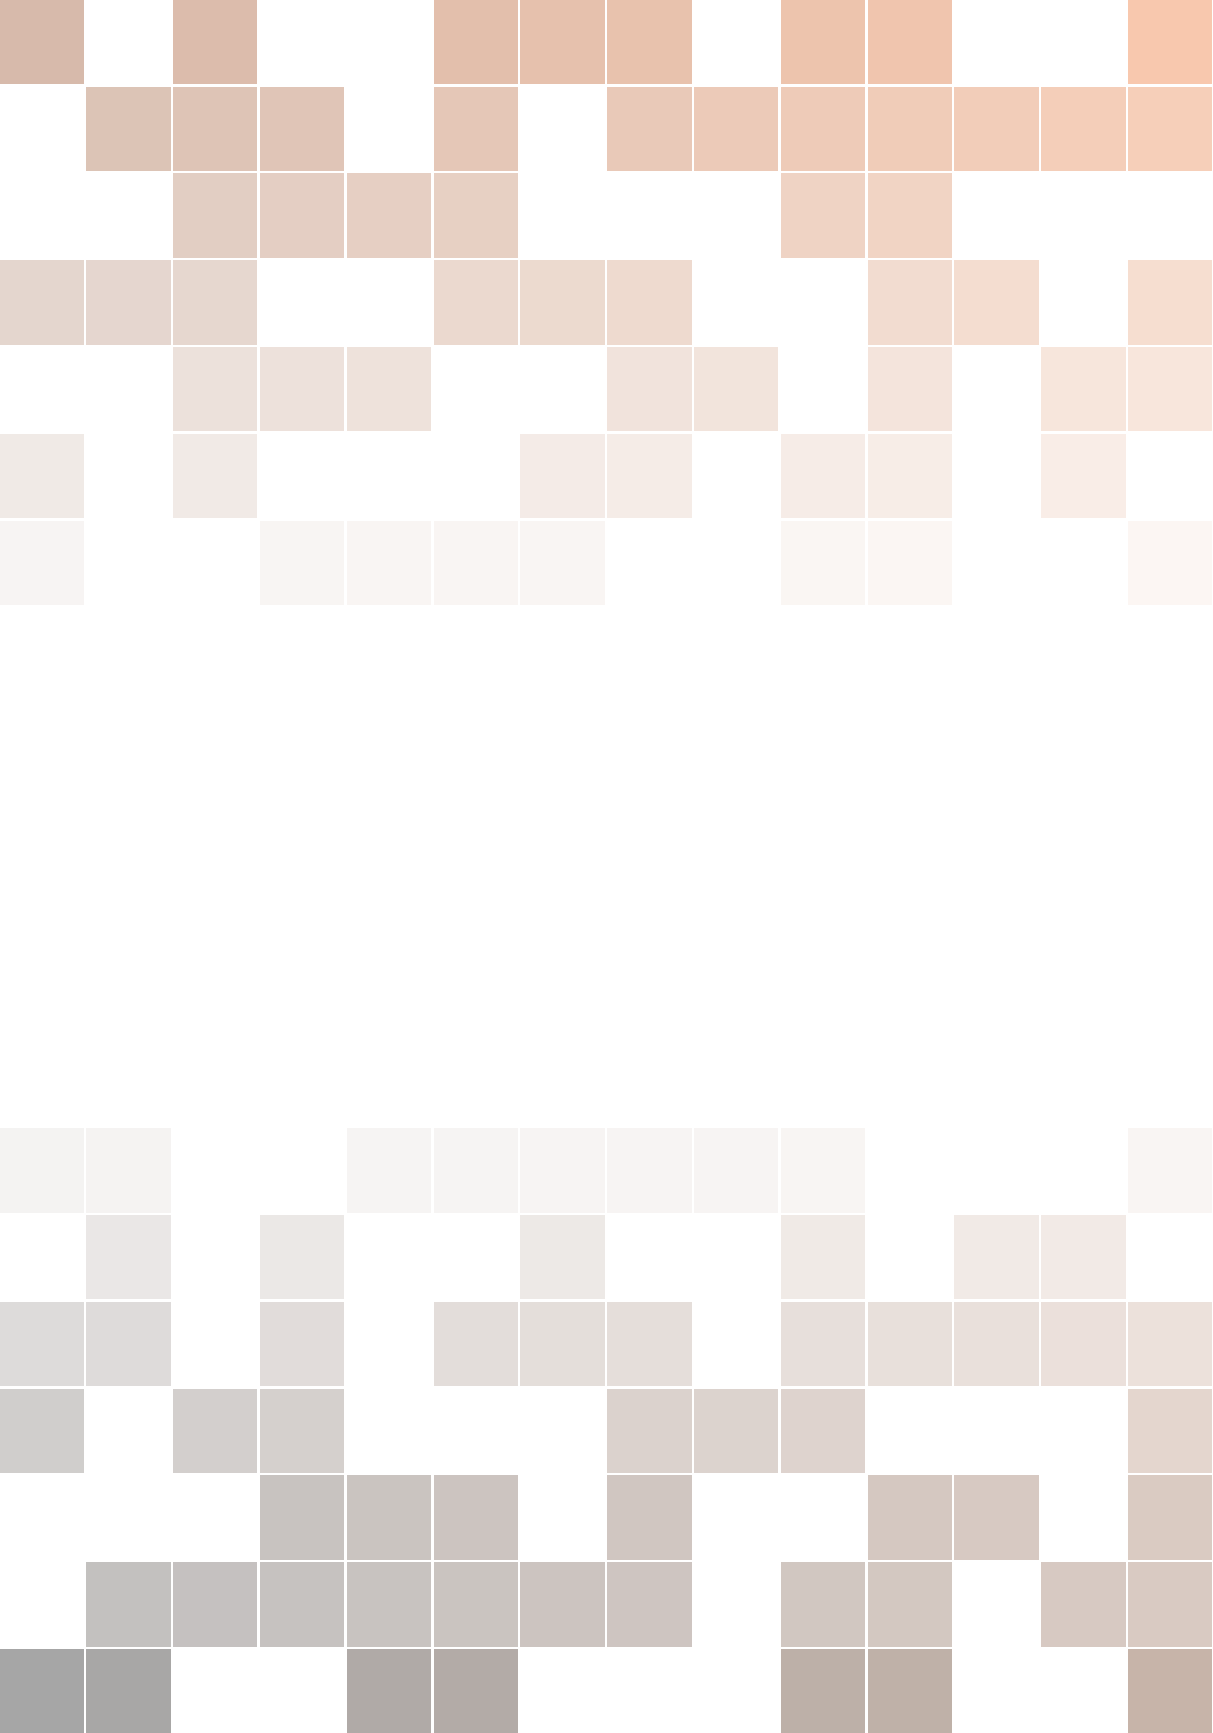
\includegraphics[width=\paperwidth]{background}}; % Background image
\draw[anchor=north] (midpoint) node [fill=orange,fill opacity=0.2,text opacity=1,inner sep=1cm]{\Huge\centering\sffamily\parbox[c][][t]{\paperwidth}{\bf \centering \zihao{-0}  热力学与统计物理导论\\[1pt] % Book title
{\bf \zihao{3} 原著:Herbert B. Callen\quad 翻译:超理汉化组}\\[1pt] % Author name
{\bf \zihao{3} \chntoday}
}};
\end{tikzpicture}};
\end{tikzpicture}
\vfill
\endgroup

%----------------------------------------------------------------------------------------
%	TABLE OF CONTENTS
%----------------------------------------------------------------------------------------
\begin{spacing}{1.4}

%\pagestyle{empty} % No headers

%%% store graphics in a box
%\newsavebox{\mygraphic}
%	\sbox{\mygraphic}{%
%		\includegraphics[keepaspectratio, height=0.2\textheight,%
%							width=0.2\textwidth]{jty.png}}
%	\AddToShipoutPicture{
%	    \put(480,0){\makebox(-15,0)[bl]{\usebox{\mygraphic}}}}

\chapterimage{chapter_head_1.pdf}
\input{Preface}

\tableofcontents % Print the table of contents itself

%\chapterimage{homura1.png}

\pagestyle{fancy} % Print headers again
\setcounter{page}{0}

\part{经典热力学基本原理}



%----------------------------------------------------------------------------------------
%	翻译:SI
%	校对:未校对!
%----------------------------------------------------------------------------------------


\chapter*{引言}
\section*{热力学本质与统计力学基础}

物理学家、化学家、生物学家或者工程师总是主要与自然界中宏观物质的性质打交道,宏观性质具有一般规律,而且具有严格的限制。表面上无关的各种性质实际有着微妙的联系。

这一潜在规律有着深远的含义。非常熟悉\sout{西方}这一套理论的物理学家与化学家在处理新材料时不至于一无所知。{\color{red} Engineers are able to anticipate limitalimitations to device designs predicated on creatively imagined (but yet undiscovered) materials with the requisite properties.} 潜在规律的具体形式则是基本物理理论的深刻线索。

一些热力学的基本概念直观上非常容易感觉。例如在比较光滑的金属碗的边缘释放一个金属球,球在碗里来回滚动,每一次来回的动能与势能之和近似守恒。不过金属球总会在碗底停下,机械能似乎消失了,但球和碗有某种可观测的变化,它们“变热”了(尽管很轻微但能感觉到)。在学习热力学之前,我们就定性地认为机械能仅仅是转化成了另一种形式(而非消失),从而使得基本定律——能量守恒成立。并且还知道生理感觉的“热”与热力学概念“温度”有关。

上述实验观测模棱两可且未经定义,然而这仍揭示了热力学与经典物理其他分支明显的不同。力学与电磁学是经典物理的两大“元典”理论。前者描述力作用于质点的动力学,后者描述力的媒介——场的的动力学。它们各自有相应的基本“定律”——力学的Newton定律(或者Lagrange或Hamilton体系),电磁学的Maxwell方程组。这两门学科余下的内容无非是解释这些基本定律的作用。

热力学相当不一样。它没有特定的适用范围,也不引入像Newton定律或Maxwell方程组那样的基本定律。与力学和电磁学的专一性相比,热力学的特点是普遍性(generality)。普遍性首先是指热力学可以应用于所用宏观凝聚态系统\mpar{“宏观凝聚态系统”的原文为``macroscopic aggregation''而非``condensed matter system'',如果``aggregation''翻译为“凝聚态”不妥的话欢迎联系我指正。},第二层含义是热力学不预言可观测量的特定的数值结果,而是对允许进行的物理过程做出限制(通过{\it 不等式}),这样在表面上无关的宏观性质之间建立联系。

热力学与其他学科对比产生的基本问题只在最后一章讨论。在那里我们会看到热力学并非以自然界新的或特定的定律为基础,而是反映{\it 所有}基本定律的共有或普遍的特征。简言之,{\it 热力学是从物理学基本定律的对称性出发的,研究物质合理性质的限制条件的科学。}\mpar{原文:thermodynamics is the study of the restrictions on the possible properties of matter that follow from the symmetry properties of the fundamental laws of physics. 诚恐翻译有误不能将原著意思尽行传达故附原文。之后同理。}

基本定律的对称性与物质宏观性质之间的联系不那么明显,并且本书不试图从前者推导出后者,而是采用本书第一版探索性的热力学形式体系,在第21章才阐述性地讨论对称性根源。但是即使是热力学这一基础的初步断言也可以帮助读者了解热力学有点不常见的形式。{\color{red} But even the preliminary assertion of this basis of thermodynamics may help to prepare the reader for the somewhat uncommon form of thermodynamic theory.}  热力学继承了它的普遍性,它的非度量性质(nonmetric nature),以及它对对称性起源的强调。


\chapter{热力学基本问题与假设}
\label{chap1}
\section{宏观测量的时间性质}
\label{sec1.1}
宏观物质最显著的特征或许是难以置信的简单性——用很少的量即可表征。例如我们去药房买“一升乙醇”,这一简单描述实际是足够的。但是从原子层面看,“一升乙醇”所指定的条件实在少得可怜,这个系统完整的数学描述包括指定所有乙醇分子的坐标、动量,以及描述每个分子内部状态的量——起码有$10^{23}$量级那么多物理量才能完整描述“一升乙醇”!如果一台电脑每1微秒在屏幕上打印一个坐标,那么$100$亿年(宇宙年龄的量级)才能打印完。神奇的是,在这$10^{23}$个原子坐标,或者它们的线性组合除了一小部分之外,在宏观上是相互独立的。那些宏观相关的一小部分称为“{\it 宏观量}”(macroscopic coordinates),或者“{\it 热力学量}”(thermodynamic coordinates)\mpar{为了与符合中文习惯,``atomistic coordinates''译作“原子坐标”,``macroscopic coordinates'', ``thermodynamic coordinates''译作“宏观量”、“热力学量”。``coordinates''根据不同习惯译成“坐标”或“(物理)量”。}。

作为一门自然科学,热力学必须要预言某些实验观测的结果,热力学预期的是合适的描述性变量,这些变量规定了热力学的范围与结构。

描述宏观物质的简单性,以及选取热力学量的标准都与宏观测量的特性有关。{\it 宏观测量与原子时间尺度相比极其缓慢,与原子空间尺度相比十分粗糙}。

进行宏观测量时,原子系统正在进行极度迅速而复杂的运动。设想一个通过单色光的干涉条纹测量细金属条长度的实验,干涉条纹在照相底片上记录下来,于是这一观测的持续时间与相机的快门速度有关——一般在$10^{-2}$秒的量级。而金属棒原子振动特征周期的量级为$10^{-15}$秒…

宏观测量不可能探测到无数个以原子周期时间尺度疯狂变化的微观量,{\it 只有一小部分原子坐标的特定组合才本质上不依赖时间,因而可以宏观测量。}

“{\it 本质上}”这个词是一个重要条件,实际上绝大多数(不是所有)可观测的宏观过程是不依赖时间的。稍微努力一点的话,人类可以观测时间尺度在$10^{-7}\, \mathrm{s}$或更短一点的过程,不过就算如此还是远大于原子时间尺度($\sim 10^{-15}$秒)。因此首先考虑{\it 极限}情况,建立有关不依赖时间的现象的理论是非常合理的。这个理论就是热力学。

{\it 根据定义,考虑到宏观测量的性质,热力学只描述宏观系统的静态。}\mpar{原文:{\it By definition, suggested by the nature of macroscopic observations, thermodynamics describes only static states of macroscopic systems.} }

在$\sim 10^{23}$个原子坐标或它们的线性组合当中,只有一小部分是与时间无关的。

守恒量是最明显的、与时间无关的热力学量:系统的能量,总动量(的分量),总角动量(的分量)。不过还有其他热力学量,为此需要讨论宏观测量的{\it 空间}性质。

\section{宏观测量的空间性质}
\label{sec1.2}
宏观测量不仅与原子时间尺度相比及其缓慢,而且在原子空间尺度上十分粗糙。用来观测宏观物质的工具总是“钝”的。例如光学仪器的分辨能力与光波长(量级约1000个原子间距)有关,因此可分辨的最小体积含有大约$10^9$个原子… {\it 宏观测量只能检测到原子坐标的空间平均值}。\mpar{原文:{\it Macroscopic observations sense only coarse spatial averages of atomic coordinates.} }

宏观测量暗含的时间空间上的两种平均大大减少了相关变量的数目:从开始的$10^{23}$个原子坐标减少为少数几个热力学量。这一减少的原理可以通过考虑如下的简单系统来扼要地解释。如图1.1,模型系统由9个原子(不是$10^{23}$个)组成,它们只能在连线上做一维运动,相互之间通过线性回复力相互作用(就像连着弹簧那样)。

{
	\centering
	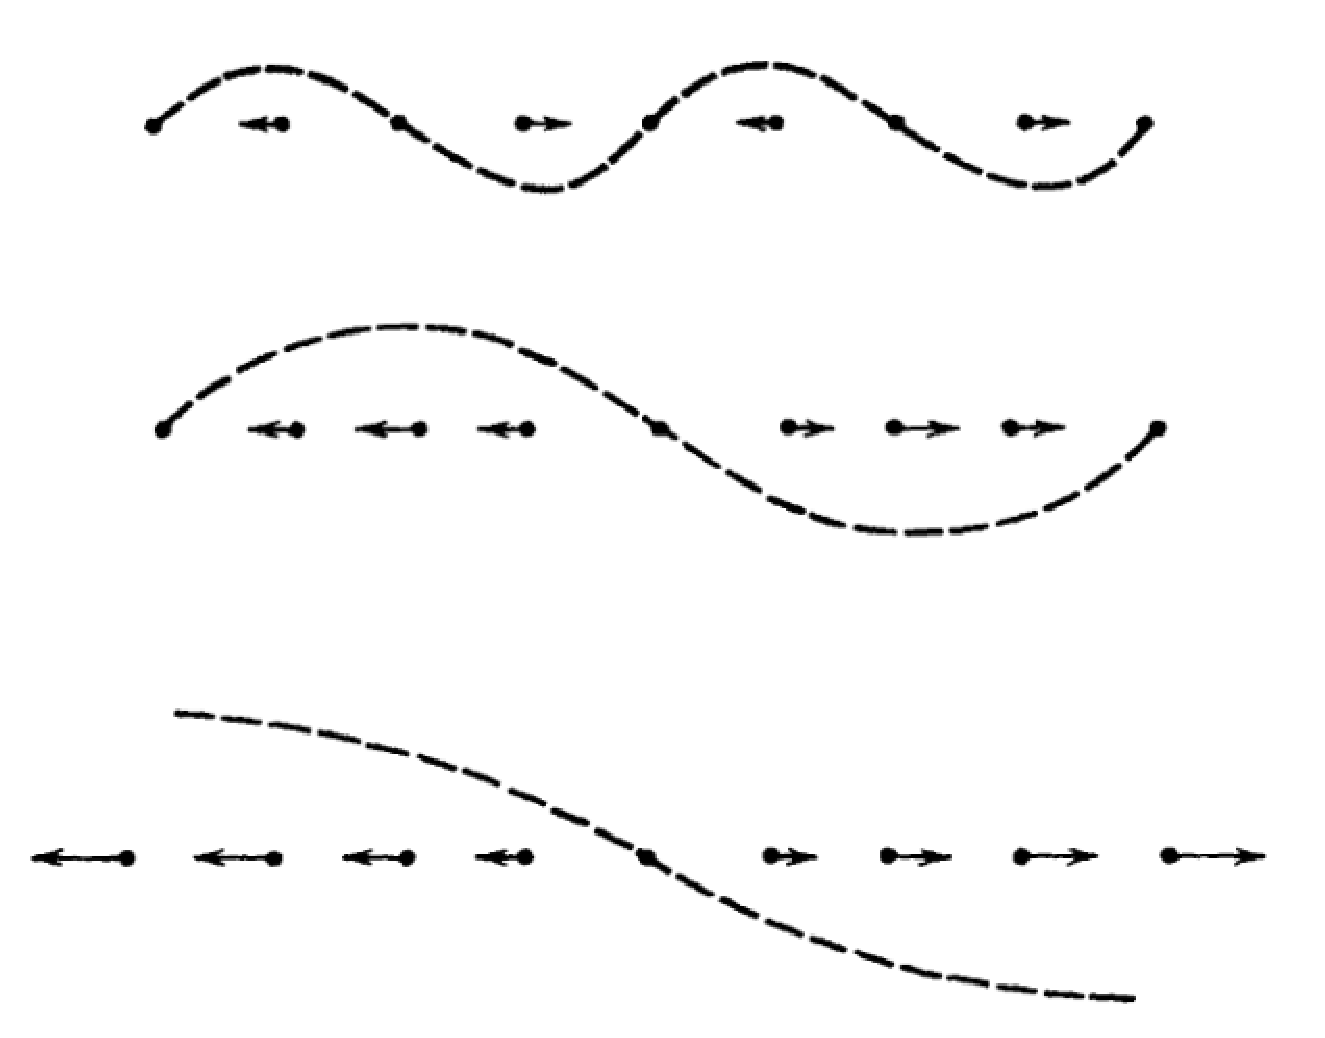
\includegraphics[scale=0.4]{fig1_1.eps} 
	\figcaption{9个原子组成的一维原子链系统的三种简正模。三种模的波长自上而下依次是4个、8个与16个原子间距。虚线表示原子纵向位移的大小。}
}

各个原子之间相互耦合,全体原子具有的规则的运动模式称为{\it 简正模式}(normal modes),简称简正模\mpar{简正模的概念参见任意一本理论力学教材,例如Herbert Goldstein, Classical Mechanics, 3rd edition,Addison Wesley, \S 6.3, Page 252.}。图1.1中显示了三种简正模的运动形式。图中的箭头方向表示原子位移方向,箭头长度表示位移大小。原子来回振动,每过半个周期图中的箭头反向。\mpar{未来会不会有一天教科书可以播放gif动图?}

给出每个原子的位置即描述了系统的原子状态,但更方便的做法是给出各种简正模的瞬时振幅(二者在数学上等价)。这些振幅称为{\it 简正坐标}(normal coordinates),且简正坐标的数量与原子坐标数目相等。

把9个原子组成的系统硬要说成“宏观系统”的话“宏观”与“原子”层面的观测就会没什么区别。为了说明,我们可以将用分辨率很低的“模糊的”仪器进行的观测作为这个系统的宏观测量。于是宏观测量的粗糙性可以类比为用分辨率低的模糊镜片的视野。这种模糊的观测无法分辨图1.1中的前两种模式的细节,这些模式不能分辨且宏观上无关。相对而言,第三种模式对应的是系统整体{\it 均匀的整体膨胀或收缩},与前两种不同,这种整体的均匀胀缩即使是“模糊镜片”也能观测到。这一模式的幅度与系统的长度有关(三维情形则为体积)。{\it 长度(体积)是一个热力学变量,空间均匀性(长波模式)结构使得它不会被宏观平均所抹除}。\mpar{原文: {\it The length (of volume) remains as a thermodynamic variable, undestroyed by the spatial averaging, because of its spatially homogeneous (long wavelength) structure.} }

宏观测量的时间平均效果与上述情形类似,系统的每一种简正模有相应的特征频率,长波模式的频率更低。图1.1第三种模式的频率是三者中最低的,如果系统原子数非常多,则长波模式的频率极低甚至趋于零(进一步讨论见21章)。故而高频的短波模式在时间平均后被抹除,而{\it 与“体积”有关的长波模式频率甚低,它在时间平均下“生存”下来,就像空间平均的情形那样}。

上述简单例子的结论其实非常普遍,只有极少具有高度对称性的原子坐标才能在宏观测量的统计平均中生存下来,它们就是宏观热力学量。一些量是力学的:系统的体积、形状参量(如弹性应变)等等,还有的来自电磁学:系统的电或磁的偶极矩、多极矩什么的。{\it 力学(包括弹性力学)研究一部分“生存”的宏观量,电磁学(包括静电学、静磁学与铁磁学)研究另一部分宏观量。}\mpar{原文: {\it The study of mechanics (including elasticity) is the study of one set of surviving coordinates. The subject of electricity (including electrostatics, magnetostatics, and ferromagnetism) is the study of another set of surviving coordinates.} }

{\it 由于宏观测量的粗糙性,系统的宏观描述与大多数原子坐标不直接相关。热力学只关心大量原子坐标的平均后的宏观量。}\mpar{原文:{\it Thermodynamics, in contrast, is concerned with the macroscopic consequences of the myriads of atomic coordinates that, by virtue of the coarseness of macroscopic observations, do not appear explicitly in a macroscopic description of a system.}} 

证明宏观系统有大量“隐藏的”原子模式的最有力证据是这些模式就像仓库一样储存能量,通过“力学模式”(即与宏观力学量有关)进行的能量传递称为{\it 机械功 (mechanical work)},通过“电磁模式”传递的能量称为{\it 电功 (electrical work)}。前者的典型代表是$-P dV$($P$为压强,$V$为体积),后者的代表为$-E_e d\mathscr{P}$($E_e$为电场,$\mathscr{P}$为电偶极矩)。这些能量传递的完整内容在力学与电磁学文献讨论。{\it 从宏观可观测模式到“隐藏”模式的能量传递同样可能进行。}\mpar{原文:{\it But it is equally possible to 
transfer energy via the hidden atomic modes of motion as well as via those that happen to be macroscopically observable.} } 相应的能量传递称为{\it 热 (heat)}。当然这只是热的形象化描述,在之后正式的体系中将会给出热的可操作的定量定义。

在进行上文的讨论后,下面建立理论所需的概念定义与惯例约定。


\section{热力学系统的组成}
\label{sec1.3}
热力学非常具有普遍性,它可以描述任意复杂体系的所有力学、电磁学与热力学性质。在一开始我们主要关注热学性质,因此系统的力学与电磁性质经常理想化或简化。这很合理,力学基本只考虑不带电而未极化的系统,而电磁学的系统没有弹性形变或其它复杂力学性质。这些学科的普遍性并未因此而降低,在各种性质分别研究透彻后,将它们结合起来处理复杂系统是比较容易的。热力学也一样,一开始我们只考虑力学、电磁学性质最平凡的系统,从而可以专注于热力学的本质内容,再之后容易结合各种理论处理复杂系统。强调一遍:接下来几章所考虑的简单系统{\it 不影响}热力学的普遍性,只是为了研究方便。

我们(暂时)只考虑如下的{\it 简单系统:宏观均匀、各向同性且不带电,体积足够大可忽略边界效应,而且无外场(如电场磁场重力场)作用。}\mpar{原文:We (temporarily) restrict our attention to {\it simple systems}, defined as {\it systems that are macroscopically homogeneous, isotropic, and uncharged, that are large enough so that surface effects can be neglected, and that are not acted on by electric, magnetic, or gravitational fields.} }

这样一个简单系统没有宏观电磁学量:系统不带电、没有电磁二极四极与多极矩。也没有所有的弹性应变以及其他类似的复杂力学量。体积$V$是一个用得到的力学参量。此外,简单系统还需要一组参量描述其{\it 化学成分}。当系统由多种物质组成时,可以用各组分的原子数作为描述化学成分的参量。为了让原子数参量的数值不那么大,我们采用参量{\it 摩尔数 (mole numbers)},定义为组分的原子数除以Avogadro常数$N_A = 6.02217 \times 10^{23}$.

摩尔数由原子数定义,这超出了纯粹的宏观物理学范围,避免这一情况的等效定义是钦点1摩尔C12同位素的质量为$12 \,\mathrm{g}$. 其它核素的摩尔质量按照C12的比例定义。表1.1列出了部分元素的摩尔质量。

\begin{center}
	\begin{table}[!htbp]
		\centering
		\caption{一些自然环境中元素(同位素混合)的摩尔质量(单位为$\mathrm{g}$). {\it 数据来自the International Union of Pure and Applied Chemistry 1969年数据.}}
		\begin{tabular}{llll}
			\toprule
			\ce{H} & 1.0080 & \ce{F} & 18.9984 \\
			\ce{Li} & 6.941 & \ce{Na} & 22.9898 \\
			\ce{C} & 12.011 & \ce{Al} & 26.9815 \\
			\ce{N} & 14.0067 & \ce{S} & 32.06 \\
			\ce{O} & 15.9994 & \ce{Cl} & 35.453 \\
			\bottomrule
		\end{tabular}
		\label{tab:tt1}
	\end{table}
\end{center}

若系统由$r$种化学成分混合而成,则这$r$种组分各自的{\it 摩尔分数 (mole fractions)}定义为$N_k / (\sum_{j = 1}^r N_j), \quad (k = 1, 2, \dots, r)$, 其中$N_i$为第$i$种组分的摩尔数。所有组分的摩尔分数之和为$1$. 系统的{\it 摩尔体积 (molar volume)}定义为$V / (\sum_{j = 1}^r N_j)$.

宏观参量$V, N_1, N_2, \dots, N_r$有一个超级重要的性质,设想把两个完全相同的系统合体为一个大系统,则大系统的体积是单个子系统体积的两倍,每种组分的摩尔数也是如此。若系统的某个物理量等于每个子系统的该物理量之和,则这个物理量称为{\it 广延量 (extensive parameters)}。广延量在热力学理论中起到关键的作用。

\section{内能}
\label{sec1.4}
能量守恒是物理学最重要的结论之一,这一信念并非一日建成的,而是经历了两个半世纪缓慢而曲折的发展。它的首次提出是在1693年,Leibniz指出地球附近重力场中质点的动能$\frac{1}{2} m v^2$与重力势能$mgh$之和才是守恒的。每当新的相互作用被引入,能量似乎就不守恒了,但是总可以添加新的数学项——一种“新能量”使得能量依然守恒。例如系统带电时,必须引入{Coulomb 相互作用能量}(静电势能)$Q_1 Q_2 / r$以及电磁场能量。1905年,Einstein将能量守恒扩展到相对论领域,引入了相对论性静质能。20世纪30年代Enrico Fermi假设【{\color{red} 原文缺失}】,目的是保证核反应过程的能量守恒。现代物理中,能量守恒是物理学基本定律时间平移对称性(它是个假设)的体现,即物理学定律在过去未来从不改变,不在时间平移$(t \to t + \text{常数})$下变化,第21章进一步讨论能量守恒的这一基础。现在我们把能量守恒作为最基本、最普遍、最重要的物理定律就可以了。

宏观系统可以视为大量电子与原子核通过复杂但确定的相互作用(服从能量守恒)结合的整体,由此可推论{\it 宏观系统具有确定的能量值,服从确定的守恒定律}\mpar{原文:{\it macroscopic systems have definite and precise energies, subject to a definite conservation principle.} }。也就是说,我们现在接受明确定义的热力学系统能量作为一种守恒定律的宏观表现形式而存在,它是一种经过高度发展之后的、经测试具有极度精确且明显完整普遍性的能量。\mpar{原文:That is, we now accept the existence of a 
well-defined energy of a thermodynamic system as a macroscopic manifestation of a conservation law, highly developed, tested to an extreme precision, and apparently of complete generality at the atomic level. 
这句话来自百度人工翻译。\sout{从翻译质量上我能想象到接到订单的那位翻译蛋疼的神情}}

下面论证热力学能量函数的存在性,论证方式与历史上的十分不同。因为热力学在原子学说被公认之前就已经蓬勃发展,宏观的能量守恒可以由纯粹的宏观方式验证。这方面的重大突破是1798年Count Rumford观察到大炮钻孔过程中的热效应。Sir Humphry Davy, Sadi Carnot, Robert Mayer, 以及最终的(1840-1850年间)James Joule 在Rumford的基础上形成了完整的论证体系。历史上热的概念的形成过程是科学理论曲折发展的经典案例,体现出新学说受到公认的巨大阻力,以及人类在处理精细抽象的问题时的智慧。对此感兴趣的读者可参考D. Roller的著作{\it The Early Development of the Concepts of Temperature and Heat}(Harvard University Press, 1950),或者阅读物理学史文献。

本书不利用Rumford与Joule的实验论证能量函数的{\it 存在性},但1.7节会通过这些实验讨论热力学能量的{\it 可测量性 (measurability)}。

无论原子还是宏观层面,具有物理意义的只是能量的差值,而非绝对的值。因此通常选定某一特定状态作为基准态,其能量规定为零。其他状态相对于基准态的能量称为系统的热力学{\it 内能 (internal energy)},通常记作$U$. {\it 内能与体积、摩尔数一样是广延量}。

\section{热力学平衡态}
\label{sec1.5}

宏观系统往往对演化历史有某种“记忆”作用。一杯搅拌过的茶还会旋转一会儿,冷加工过的钢材硬度增加。但记忆终将褪色,扰动总会衰减,内应变屈服成塑性流\mpar{原文:internal strains yield to plastic flow.},不均匀的浓度扩散成一致。系统倾向于演化到与特定的过往条件无关的简单状态。

某些情形中系统很快平息到简单态,另外一些情况的演化过程则慢得要命。但是{\it 所有系统都有向如下特征状态演化的趋势:由系统内部因素决定,与先前的外部影响无关。根据定义,这种简单的终态不依赖时间。这种状态称为平衡态。}\mpar{原文:{\it in all systems there is a tendency to evolve toward states in which the properties are determined by intrinsic 
factors and not by previously applied external influences. Such simple terminal states are, by definition, time independent. They are called equilibrium states.} }

热力学致力于描述这种系统最终演化到的简单、静止的“平衡”状态。

为了将上面的定性陈述转化为定量的正式假设,我们将“简单”的标准设定为使用很少的热力学量即可描述系统。由此引出下面的假设,该假设还受到实验观测的启示,它所导出的理论的正确性验证了它自身的正确性。

\paragraph{假设 \uppercase\expandafter{\romannumeral1}.}
{\it 任意简单系统存在宏观上由内能$U$,体积$V$与各组分摩尔数$N_1, N_2, \dots, N_r$完全确定的宏观状态,称为平衡态。}

\paragraph{Postulate \uppercase\expandafter{\romannumeral1}.}
There exist particular states (called equilibrium states) of simple systems that, macroscopically, are characterized completely by the internal energy $U$, the volume $V$, and the mole numbers $N_1, N_2, \dots, N_r$ of the chemical components. 

\ 

当考虑更一般的、具有更复杂力学电磁学性质的系统时,确定一个平衡态所需的参量也相应增加,例如系统的电偶极矩或弹性应变。新变量的形式体系与简单系统的体积$V$十分相似。

实验中经常要判断一个系统是否处于平衡态,因而是否可以用热力学进行分析。首先可以观察该系统是否不再活动、处于静态,但“不活动”不是平衡态的充分条件。平衡态由广延量$U, V, N_1, N_2, \dots, N_r$完全确定,故而与演化历史无关,这很难在实际中判断。而且许多系统的演化{\it 显然}与历史有关,这些情形促使我们考虑平衡态的意义。例如,两块相同的钢材经历不同的冷加工、淬火和退火过程最终的性质可以十分不同,因而它们不处于平衡态。类似的,玻璃的性质取决于加工过程(如冷却速率),玻璃也不在平衡态。

(基于平衡态的)热力学理论强行分析非平衡态系统就会在将来的报道上出现偏差,实验者根据理论失效(后验标准)判断系统处于非平衡态。

量子统计理论通常会对热力学失效的情形中系统为何不处于平衡态作出更深刻的解释。偶然出现的理论失效往往蕴藏着系统在微观层面未知的复杂过程。例如正氢(orthohydrogen)与仲氢(parahydrogen)\footnote{正氢分子\ce{H2}两个氢核的角动量平行,仲氢的反平行。处于平衡态氢气系统的正氢/仲氢比例应该是定值,但热力学的预言失败了,这促使正氢、仲氢微观性质的研究。}的发现,及其微观机制的研究。

一个给定的宏观平衡态(因而给定了系统的边界条件)对应许多微观态,在原子层面上,处于平衡态的系统仍在对应的众多微观态中不断而迅速地转变。转变的速度往往很快,使得宏观测量过程中系统经历各种可能的微观态,这就是系统处于平衡的情况。然而在某些特殊情况下,各微观态的遍历机制失效,系统只能限制在某一特定的微观态的子集中演化转变。或者系统仍可遍历各态,但转变速度较慢,以至于宏观测量结果并非对所有微观态的平均。这些情况的系统都不是平衡态。容易看出,这些奇异情况更容易出现在固体,而非流体(液/气)系统,因为后者相对而言原子的移动性更强,原子随机碰撞强烈消除了微观态遍历限制。

实际上很少有系统处于绝对的平衡态。例如放射性物质的绝对平衡态要求完全衰变为最稳定的同位素,这需要宇宙年龄量级的时间,这种慢的要命的过程可以近似视为平衡态。完成了自发演化、可以用相对较少的参量描述的系统可认为处于{\it 亚稳态 (metastable equilibrium)}。这种稍弱的平衡状态对热力学的应用而言是足够的。

综上,实践中的平衡态判据是循环的。{\it 若热力学理论成功描述了一个系统,则该系统就处于平衡态!}\mpar{原文:{\it Operationally,a system is in an equilibrium state if its properties are consistently described by thermodynamic theory!}}

应该指出,上述\sout{耍流氓的}循环逻辑与力学的情形{\it 没有}不同。例如力学预言质点在已知的引力场中沿特定轨迹运动,如果报道出了偏差,没人会因此否定力学,而是会推测质点受到其他的力。例如如果粒子带电,则考虑电磁力之后动力学预言才正确,这只有通过循环一圈(预言-出了偏差-加上电磁力-预言成功)才推论得知,因而不是先验的。力学系统模型(如质量、转动惯量、电荷、电偶极矩等等)与实验符合之后才是“正确”的。

\section{壁与限制}
\label{sec1.6}
一个热力学系统需要一个“壁”(walls)来将它从周围环境中隔离出来,并为它提供边界条件。通过对壁进行操作,可以改变系统的广延量,以及开始某些演化过程。

通过对壁进行操作而开始的过程通常是某些物理量在不同系统或大系统的子体系之间的重新分布。由此可将热力学壁分为允许或禁止重新分布两种。例如,考虑一个刚性圆筒内部的活塞,如果活塞是固定的,则它是禁止两个子系统的体系重新分布的壁,若活塞可以活动,则允许体积重新分布。刚性圆筒与固定的活塞称为{\it 限制}体积的壁,而可动活塞对体积是非限制的。一般的,将一个系统的某个广延量限制为特定值的壁称为对该广延量有限制,而允许该量自由改变的壁对该广延量是非限制的。

系统的某种化学组分不能渗透的壁限制了该组分的摩尔数;而可以透过的膜对摩尔数无限制。半透膜限制特定组分的摩尔数而对其他成分无影响;一个有孔的壁对任意组分的摩尔数都无限制。

要考虑限制能量的壁是否存在需要先解决能量的可测量性问题,下一节就讨论它。

\section{能量的可测量性}
\label{sec1.7}
基于原子层面的能量守恒可以推论出存在守恒的宏观能量函数。为了证明能量具有实际意义,必须说明它是{\it 可控制的(controllable)}与{\it 可测量的(measurable)}。下面我们首先指出存在测量能量的定量方法,并据此导出热的定量的操作性定义。

论证能量可测量性的关键是绝热壁的存在。下述的简单实验表明存在这种绝热壁。

考虑盛有冰水混合物的容器。实验发现剧烈搅拌容器可使得冰迅速融化,搅拌过程向系统传递了机械功,由此可推论冰的融化与系统能量增加有关。将容器放在夏日的阳光下可以发现冰自然地迅速融化了,该过程外界并未对系统做功,因此可以认为能量通过传热的形式进入系统中。将容器壁从薄金属换成厚玻璃,再换成Dewar瓶壁(两层镀银的玻璃,中间抽真空)会发现冰融化的越来越慢,这强烈暗示金属、玻璃与Dewar壁的隔热性越来越好。机智的实验家可以制造性能超好的隔热壁使得冰的融化速度十分慢,这种壁是理想绝热壁在三次元现实的良好近似。

通常称不透热的壁为{\it 绝热的 (adiabatic)},而允许热传递的壁称为{\it 导热的 (diathermal)}。如果系统的壁既不传递做功也不导热,则它可以{\it 限制系统的能量}。若系统的壁限制能量、体积与所有组分的摩尔数,则称这个系统是{\it 封闭的 (closed)}\footnote{本书的封闭性的定义与化学中的惯例不同,化学的封闭性只是限制系统组分的摩尔数不变。}。

利用上述几种壁可以论证宏观热力学能量的{\it 可控制性},比如可以用绝热壁关住能量,用透热壁使能量流动。再比如将系统用限制能量的壁封印起来的话,该系统明天的能量也可以确定。没有这些壁的话,热力学就成了空谈的纯理论了。

下面讨论能量的{\it 可测量性},更确切的说,是讨论(具有物理意义的)能量差的可测量性。被绝热壁包围的简单系统只可能通过做功的方式向它传递能量。机械功可根据力学理论计算。例如压缩活塞做的功等于力乘以位移,用杆搅拌的功等于力矩乘以角位移。这种情况的功在力学里已经完备地讨论了定义与测量方法。由此可得,{\it 如果系统被绝热壁包围,并通过做机械功从一个状态达到另一个状态,}则这两个状态的能量差即为所做机械功的值。\mpar{原文:we are able to measure the energy difference of two states {\it provided that one state can be reached from the other by some mechanical process while the system is enclosed by an adiabatic impermeable wall.}} 

例:考虑刚性绝热容器中达到平衡态的冰水混合物系统。在壁上开一个小洞穿过一个杆,杆的一侧是桨,另一侧是曲柄,这样就能通过转动曲柄对系统做机械功,机械功等于力矩乘以角位移。转一段时间后,系统达到新的平衡态(一些冰融化了)。系统末态减初态的能量差即为转动曲柄做的功。

还有一个问题。将系统由绝热壁包围\mpar{如无特别说明,本节涉及的壁都是不可透过物质的(impermeable)。},初状态任意,它能否只通过做机械功达到任意指定的末态?这要借助Joule完成的实验,他的工作表明{\it 绝热系统摩尔数$N_1, \dots, N_r$相等的任意两个状态,都存在力学过程将它们联系起来}。\mpar{原文:{\it system enclosed by an adiabatic impermeable wall any two equilibrium states with 
the same set of mole numbers $N_1, N_2,..., N_r$. can be joined by some possible mechanical process.} } Joule还发现给定(绝热系统的)两个状态(记作$A, B$)后,从$A \to B${\bf 或者}$B \to A$的力学过程至少存在一个,但其中的某一个(比如$A \to B$)可能不存在。我们的目的是测量状态的能量差,因此存在一个过程就够用了。综上,{\it 借助机械功可以测量摩尔数相同的任意两个状态的能量差。}

Joule观察到的只有$A \to B$或$B \to A$一个过程存在的情形具有深刻意义。这两个状态的不对称性是{\it 不可逆性 (irreversibility)}概念的体现,后面会深入讨论。

上述测量能量差的方法的唯一限制是初末状态摩尔数相同。这可以由如下方式解决:考虑由挡板(物质不可透过)隔开的两个子系统,它们的相对于基准态的能量可由上述方法测出。移除挡板,子系统混合,并且二者的总能量守恒。因此混合系统的终态能量等于两个子系统的初态能量之和。这样就可以测量摩尔数不同的状态间的能量差。

总结:{\it 利用绝热壁与机械功可以测量热力学系统任意状态相对于基准态的能量。}\mpar{原文:{\it by employing adiabatic walls and by measuring only mechanical work, the energy of any thermodynamic system. relative to an appropriate reference state, can be measured. } }

\section{热的定量定义}
\label{sec1.8}
利用任意两平衡态的能量差的可测量性,可以对热进行定量定义:{\it 系统在某一(摩尔数不变)过程中外界流入系统的热量定义为系统末态与初态的能量差减去外界对系统做的功。}\mpar{原文:{\it The heat flux to a system in any process (at constant mole numbers) is simply the difference in internal energy between the final and initial states, diminished by the work done in that process. } }

设系统经某一过程由初态$A$演化为末态$B$,该过程中外界对系统做的功以及外界传递给系统的热量是多少?前者根据力学理论不难计算。根据\ref{sec1.7}节介绍的方法可得能量差$U_B - U_A$,从能量差中减去机械功即可得该过程中传递给系统的热流。

应该指出,相同的初末状态对应的不同过程的做功大小可以不同,同样,传热大小也可以不同,但是做功与传热的和——能量差$U_B - U_A$在初末态给定后对所有过程都是相等的。计算能量差只需给定初末状态,而计算做功、传热大小必须给出联系初末态的特定过程。

外界对简单热力学系统通过改变体积所做的准静态功为:
\begin{equation}
\label{equ1.1}
	\delta W_M = -P dV
\end{equation}
其中$P$为系统压强。上式不难从力学导出,必须强调上式只适用于{\it 准静态过程 (quasi-static processes)}。准静态过程的准确定义在\ref{sec4.2}节讨论,这里只进行定性解释。考虑一个带有可移动活塞的气缸,气缸内封闭有一定气体。迅速压动活塞,则在活塞附近的气体立即获得动能,气体出现湍流,压强无法定义。这种过程不是准静态的,对系统做的功也不能由\eqref{equ1.1}式计算。如果以极其慢(准静态地)速率推动活塞,则系统在每一时刻都可视为处于静平衡态,\eqref{equ1.1}式可以使用。粗略地说,“无穷慢”即为准静态过程的本质。

\eqref{equ1.1}式的符号惯例值得注意。若系统的能量增加,则外界对系统做正功。若系统体积减少,则外界对系统做正功,使系统的能量增加,因此\eqref{equ1.1}式等号右侧有个负号。

利用准静态功的定量表述$\delta W_M = -PdV$可导出传热的定量公式,一个摩尔数不变的无穷小准静态过程中传递给系统的{\it 准静态热量 (quasi-static heat)}$\delta Q$定义为:
\begin{equation}
\label{equ1.2}
	\delta Q = dU - \delta W_M, \quad \text{摩尔数不变。}
\end{equation}
或者:
\begin{equation}
\label{equ1.3}
	\delta Q = dU + P dV, \quad \text{摩尔数不变。}
\end{equation}
{\it 热量 (heat)}与{\it 热流 (heat flux)}这两个术语经常混用,因为热量就像功那样,是能量的{\it 传递 (transfer)}形式。能量被传入系统之后就不能分辨是通过做功还是传热传给系统的,尽管$dU$分为$\delta Q$与$\delta W_M$两部分,但能量$U${\it 不能}分为“做功”部分与“传热”部分。我们采用符号$\delta$表示无穷小做功与传热,$\delta Q$与$\delta W_M$称为{\it 不完整微分 (imperfect differentials)}。$\delta W_M$与$\delta Q$沿某一特定过程进行积分得到{\it 该过程}的做功与传热值,而它们的和——能量差$\Delta U$与具体过程无关(只与初末状态有关)。

热量,功与能量的概念可通过如下的类比来说明。设一位农场主有个池塘,一条溪流注入池塘,另一条从池塘流出。池塘还通过降雨获得水分、通过蒸发流失水分(“负降雨”)。将池塘比作热力学系统,水量视为系统内能,溪流注入流出类比成做功,降雨蒸发当做传热。

首先,在任何时刻,池塘的水不能分成来自降水与来自溪流的部分。{\it 降雨}只是水{\it 转移}的形式。\mpar{如同热是能量转移的形式。}

然后考虑测量池塘水量的方法。可以使用流量计测量流入流出池塘的溪流水量,但是对降雨而言没有那样的雨量计。为了测量降雨量,可以用防水布将池塘覆盖(类比{\it 绝热壁}),使得降雨和蒸发不能改变水量。将一带刻度的长直杆垂直插入池塘以记录水位变化,通过在两条溪流筑坝即可控制池塘水位,结合流量计与刻度杆即可测定池塘水量($U$)。因此在防水布(绝热壁)的帮助下,池塘任意水位(状态)的水量(内能)都可测定\mpar{当然,就像\ref{sec1.7}节只是测定系统任意状态{\bf 相对于基准状态}的能量那样,这里只测定池塘的任意水位相对于某一基准水位对应的水量。}。

把防水布撤去从而使降水可以影响池塘水量,要得到某一过程中降水导致的水量变化,可以通过如下间接方式。首先从刻度杆上读出水位的变化,从而水量的变化可以由上一段的方法得出。然后根据流量计测量溪流造成水量的变化。水量的变化减溪流造成的变化即为降水量。读者不难看出其中的类比关系。

因为做功与传热都是能量传递的形式,故功和热量的都是能量的单位。能量在cgs单位制\mpar{cgs: centimeter-gram-second单位制,或者厘米-克-秒单位制,又称高斯单位制。}中的单位是erg(尔格),在mks单位制\mpar{mks: metre-kilogram-second单位制,或者米-千克-秒单位制,又称国际单位制。}中为joule (焦耳),记作J,二者的关系为$1\, \mathrm{J} = 10^7\, \mathrm{erg}.$

常用的能量单位还有calorie(卡,1 cal = 4.1858 J)\footnote{营养学家习惯把一千calorie简记为``Calorie''(这使得能量的数值合适不至于太大),但要命的是他们经常忘了大写字母C,于是一千calorie成了一``calorie''!}。历史上,calorie是在热与功的关系澄清之前所用的热量单位,直到现在,还有人只用calorie计量热量、用joule计量功。然而calorie与joule都是能量单位,它们描述功与热量都是可以的。

其他的能量单位制还有英国热量单位(the British thermal unit, Btu),升—大气压单位(liter-atmosphere),英尺—磅单位(foot-pound)与瓦特—时单位(watt-hour)。各单位制能量单位间的转换参见本书封底。

{\bf {\large 例 1}}
\ 

带有可移动活塞的气缸内封印着一定气体。通过观测发现,气体在绝热过程中满足:
\[
	P^3 V^5 = \text{constant}, \quad (\delta Q = 0)
\]

\begin{enumerate}
	\item[(a)] 求下图$ADB, ACB, A \stackrel{ \text{直线} }{\longrightarrow} B$三个过程中外界对系统做的准静态功、外界传递给系统的热量。


	{
		\centering
		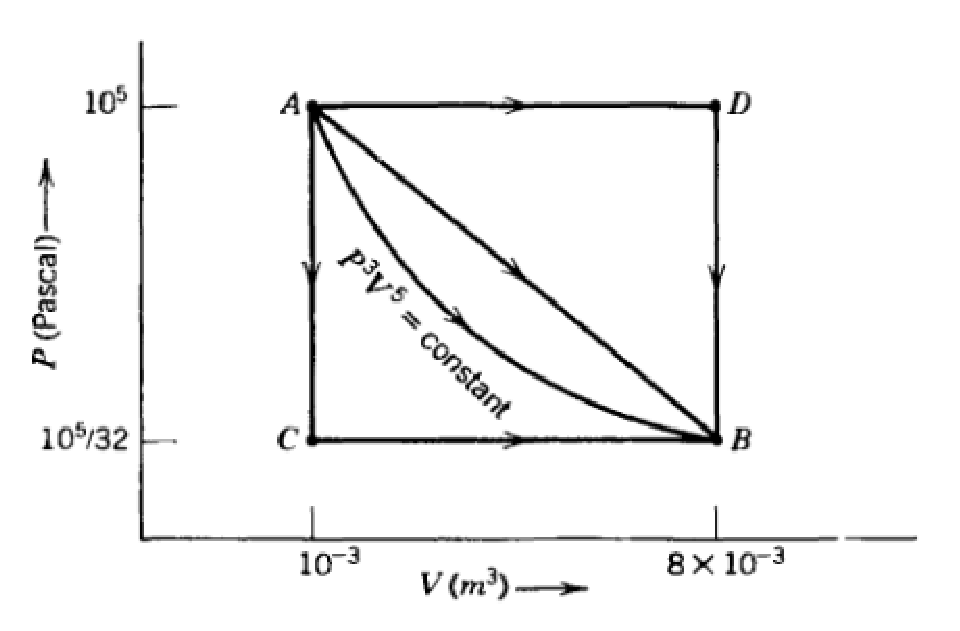
\includegraphics[scale=0.7]{fig1_8.eps}
		\notag
	}

	在$ADB$过程中气体保持压强不变($P = 10^5 \, \mathrm{Pa}$)被加热,从初始体积$10^{-3} \, \mathrm{m}^3$变为末态体积$8 \times 10^{-3} \, \mathrm{m}^3$. 然后保持体积不变,将气体冷却至压强降为$10^5 / 32 \, \mathrm{Pa}$。同样,其他过程($ACB, AB$)的具体内容由图不难看出。

	\item[(b)] 在系统内安装一个由发动机驱动的桨,在发动机提供的力矩作用下桨以均匀角速度$\omega$转动,观测到气体系统(体积不变)压强的变化率为:
	\[
		\frac{dP}{dt} = \frac{2}{3} \frac{\omega}{V} \times \text{力矩}
	\]
	求证系统任意两个体积相等的状态的内能差可通过该过程计算。算出$U_C - U_A$和$U_D - U_B$.

	这个过程只能单向进行(只能从$P-V$图垂直向上而不能向下进行),这是为啥?

	\item[(c)] 求证系统的任意两个平衡态(即$P-V$图中的任意两点)可通过(a)、(b)描述的两个过程联系起来。计算$U_D - U_A$.

	\item[(d)] 计算图中$A \to D$过程外界对系统做的功$W_{AD}$以及传递给系统的热$Q_{AD}$. 计算$D \to B, C \to A$过程同样的量,并说明这些计算结果与(a)一致。
\end{enumerate}

读者在参考下面的答案{\it 之前}应该先尝试解答这些题目。

\ 

{\it \large 解答}

\begin{enumerate}
	\item[(a)] 
		利用绝热条件$Q = 0, \Delta U = W$以及$P^3 V^5 = \mathrm{constant}\, \quad (Q = 0)$可得:
	\begin{align*}
		U_B - U_A &= W_{AB} = -\int_{V_A}^{V_B} PdV = -P_A \int_{V_A}^{V_B} \left( \frac{V_A}{V} \right)^{5/3} dV \\
		&= \frac{3}{2} P_A V_A^{5/3} \big( V_B^{2/3} - V_A^{2/3} \big) \\
		&= \frac{3}{2} (25 - 100) \,\mathrm{J} = -112.5\, \mathrm{J}.
	\end{align*}
		考虑$ADB$过程:
		\begin{align*}
			W_{ADB} &= -\int PdV = -10^5 \times (8 \times 10^{-3} - 10^{-3}) \,\mathrm{J} = -700 \,\mathrm{J} \\
			U_B - U_A &= W_{ADB} + Q_{ADB} \\
			Q_{ADB} &= (-112.5 + 700) \,\mathrm{J} = 587.5 \,\mathrm{J}.
		\end{align*}
		尽管能算出$Q_{ADB}$,但不能分别得到$Q_{AD}, Q_{DB}$,因为还不知道$U_D - U_A$.

		其他过程的计算同理。答案是$W_{ACB} = -21.9 \,\mathrm{J}, Q_{ACB} = -90.6 \,\mathrm{J}; W_{AB} = -360.9 \,\mathrm{J}, Q_{AB} = 248.4 \,\mathrm{J}$.
	\item[(b)] 
		电动机的力矩使桨旋转角度$d\theta$传递给系统的能量\footnote{注意电动机传递能量给系统既不是做功也不是传热的方式——这是一种{\it 非准静态 (non-quasi-static)}的能量传递。 }为$dU = \text{力矩} \times d\theta$, 另外$d\theta = \omega dt$,因此
		\begin{align*}
			dP &= \frac{2}{3} \frac{1}{V} \cdot \text{力矩} \cdot \omega dt \\
			&= \frac{2}{3} \frac{1}{V} dU \\
		\end{align*}
		整理得
		\[
			dU = \frac{3}{2} VdP
		\]
		$dU = \text{力矩} \times d\theta \to dU \geq 0$($d\theta$与力矩符号相同),再结合$V > 0$可得$dP \geq 0$,因此该过程只能向压强增大的方向单向进行。

		\begin{align*}
			U_A - U_C &= \frac{3}{2} V (P_A - P_C) = \frac{3}{2} \times 10^{-3} \times \left( 10^5 - \frac{1}{32} \times 10^5 \right) = 143.5 \,\mathrm{J} \\
			U_D - U_B &= \frac{3}{2}
		\end{align*}
	\item[(c)]
		任意给定$P-V$图上两点,为了将它们联系起来,过其中任意一点画一条绝热线(绝热过程对应的线),再过另一点画等容线($V = \text{常数}$),这两条线相交,于是两个过程联系起来。

		前面已经利用绝热过程求出$U_B - U_A = -112.5 \,\mathrm{J}$,利用不可逆的搅拌过程求出$U_D - U_B = 1162.5 \,\mathrm{J}$。因此$U_D - U_A = 1050 \,\mathrm{J}$。等价地,可以将状态$A$设为基准态,则
		\[
			U_A = 0, \quad U_B = -112.5 \,\mathrm{J}, \quad U_C = -145.3 \,\mathrm{J}, \quad U_D = 1050 \,\mathrm{J}.
		\]
	任意状态的内能$U$都可以求出。
	\item[(d)]
		已经计算出了$U_D - U_A$以及$W_{AD}$,由此可得$Q_{AD}$:
		\begin{align*}
			U_D - U_A &= W_{AD} + Q_{AD} \\
			1050 \,\mathrm{J} &= -700 \,\mathrm{J} + Q_{AD} \\
			Q_{AD} &= 1750 \,\mathrm{J}
		\end{align*}
		同样
		\begin{align*}
			U_B - U_D &= W_{DB} + Q_{DB} \\
			-1162.5 \,\mathrm{J} &= 0 + Q_{DB}.
		\end{align*}
		为了检验,计算$Q_{AD} + Q_{DB} = 587.5 \,\mathrm{J}$,等于在(a)中计算的$Q_{ADB}$,nice!
\end{enumerate}

\subsection*{习题\mpar{译者水平有限只敢列出原文有答案的习题的解题过程……(没答案的不知道对错不敢放上去)}}
\begin{enumerate}
	\item[1.8-1.]
		计算本节例1中系统状态$(P = 5 \times 10^4 \,\mathrm{Pa}, V = 8 \times 10^{-3}\, \mathrm{m}^3)$对应的内能。

		{\it
			以状态$A$为参考状态,即设$U_A = 0$.

			记$(P = 5 \times 10^4 \,\mathrm{Pa}, V = 8 \times 10^{-3}\, \mathrm{m}^3)$为状态$E$. 因$V_B = V_E$,故可通过例1(b)描述的不可逆搅拌过程从$E$演化到$B$态:
			\begin{align*}
				E \stackrel{{\text{不可逆搅拌}} }{\longrightarrow} B \\
				U_B - U_E &= \frac{3}{2} V_E (P_B - P_E) \\
				&= \frac{3}{2} \times 8 \times 10^{-3} \times \left( \frac{1}{32} \times 10^{5} - 5 \times 10^{4} \right) \,\mathrm{J} \\
				&= -562.5 \,\mathrm{J}.
			\end{align*}
			由例1(c),以$A$为参考态时,$U_B = -112.5 \,\mathrm{J}$,故 
			\begin{equation*}
				U_E = \big(-112.5 - (-562.5) \big) \,\mathrm{J} = 450 \,\mathrm{J}.
			\end{equation*}
		}
	
	\item[1.8-2.]
		还是例1的条件。记上一问的状态$(P = 5\times 10^4 \,\mathrm{Pa}, V = 8 \times 10^{-3} \,\mathrm{m}^3)$为$X$,计算系统从状态$A$沿$P-V$图的直线演化到状态$X$过程中吸收的热量。

	\item[1.8-3.]
		某一气体系统的能量为:
		\[ U = 2.8 PV + \text{constant}. \]
		系统的初始状态为$P = 0.2\, \mathrm{MPa}\ (10^{6} \mathrm{Pa}), V = 0.01\, m^3$,对应下图中的A点。系统经历图中的循环过程($A \to B, B \to C, C \to A$)。计算每个过程中系统的吸热量$Q$与外界对系统做的功$W$。
		
		
		{
			\centering
			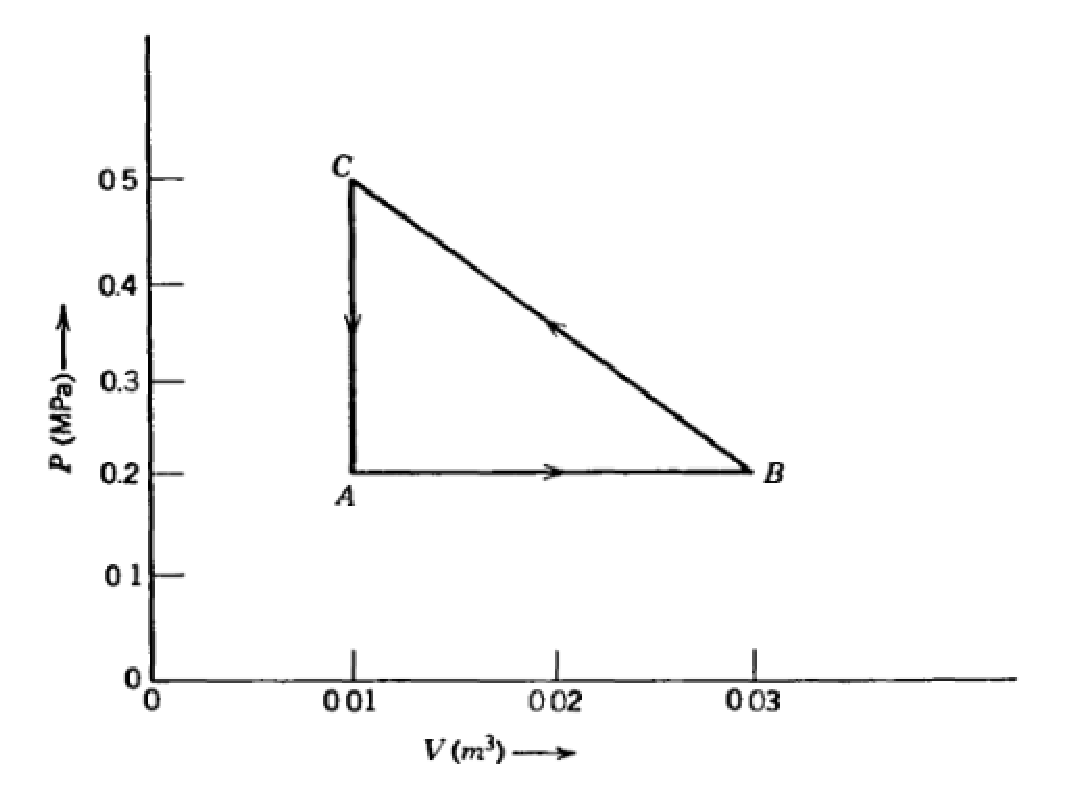
\includegraphics[scale=0.6]{fig1_8_3.eps}
			\notag
		}
		
		
		{\it
			以$B \to C$过程为例(答案只给了$BC$过程的……)
		
			状态$B$:$V = 0.03\, \mathrm{m}^3, P = 0.2 \mathrm{MPa}$.

			状态$C$:$V = 0.01 \,\mathrm{m}^3, P = 0.5 \,\mathrm{MPa}.$

			直线 $BC$: $P = (-15\, \mathrm{MPa \, m^{-3}}) V + 0.65\, \mathrm{MPa}$.

			\[ W_{BC} = -\int_{V_B}^{V_C} PdV = -\int_{0.03}^{0.01} (-15V + 0.65) dV = 7 \times 10^3 \,\mathrm{J}. \]

			\[ U_C - U_B = 2.5(P_C V_C - P_B V_B = 2.5(0.5\times 0.01 - 0.2 \times 0.03) \,\mathrm{MJ} = -2.5 \times 10^3 \,\mathrm{J}. \]

			\[ Q_{BC} = (U_C - U_B) - W_{BC} = (-2.5 \times 10^3) \,\mathrm{J} - 7 \times 10^{3} \,\mathrm{J} = -9.5 \times 10^3 \,\mathrm{J}. \]
		}

	\item[1.8-4.]
		求习题1.8-3中的系统在绝热过程中的$P-V$曲线,即求$P = P(V)$使得沿这条线的过程满足$\delta Q = 0$。

		{\it
			外界对系统做的功为
				\[ W = -\int_{V_0}^{V} P(V') \, dV'. \]
			绝热过程中系统吸热$Q = 0$,故内能变化量$U = W$。由1.8-3中条件\mpar{$U = 2.5 PV + \mathrm{constant}$. }可知,初末状态的内能差为:
				\[ U = 2.5(P V - P_0 V_0). \]
			联立得
				\begin{align*}
					2.5 (PV - P_0 V_0) = -\int_{V_0}^V P(V') \, dV' \\
					= 2.5 \left(P + \frac{dP}{dV} V \right) = -P(V) \\
					\frac{dP}{dV} = -\frac{7}{5} \frac{P(V)}{V} \\
					\to P \propto V^{-7/5} \\
					\to P^5 V^7 = \mathrm{constant}.
				\end{align*}
		}
	\item[1.8-5]
		单位摩尔数物质的某系统的内能为
		\[ U = AP^2 V. \]
		其中$A$是正的常数,量纲为$[\mathrm{P}]^{-1}$. 求$P-V$图绝热线的形式。

	\item[1.8-6]
		实验观测发现某系统保持体积$V_0$不变,压强从$P_0$变化到任意值$P'$时,系统吸收的热量为
		\[ Q' = A(P' - P_0) \quad(A > 0). \]
		此外,系统在绝热过程满足:
		\[ P V^\gamma = \text{constant} \quad (\gamma\text{是正的常数}) \]
		求任意状态的内能$U(P, V)$. (用已知量$P_0, V_0, A, U_0 \equiv U(P_0, V_0)\text{与} \gamma$,当然还有自变量$P, V$表示)

		{\it
			\[ A: (V_0, P_0), \quad B: (V_0, P_B), \quad C: (V, P). \]
			构造如下状态使得系统从初态$A$演化到末态(任意状态)$C$:
			\[ A \stackrel{\text{定容过程}}{\longrightarrow} B \stackrel{\text{绝热过程}}{\longrightarrow} C. \]

			$A \stackrel{\text{定容过程}}{\longrightarrow} B$: 
				
			$W_{AB} = 0, Q_{AB} = A(P_B - P_0)$,
			\[ U_B - U_A = W_{AB} + Q_{AB} = A(P_B - P_0). \]

			$B \stackrel{\text{绝热过程}}{\longrightarrow} C$: 
				
			$Q_{BC} = 0$.
			\[ P V^\gamma = P_B V_0^\gamma \to P = \frac{P_B V_0^\gamma}{V^\gamma}. \]
			\[ W_{BC} = -\int_{V_0}^{V} \frac{P_B V_0^\gamma}{V'^\gamma} \,dV' = -P_B V_0^\gamma \frac{V^{-\gamma + 1} - V_B^{-\gamma + 1}}{-\gamma + 1}. \]
			\[ U - U_B = Q_{BC} + W_{BC} = -P_B V_0^\gamma \frac{V^{-\gamma + 1} - V_0^{-\gamma + 1}}{-\gamma + 1}. \]

			因此初末状态内能差为
			\begin{align*}
				U - U_0 &= (U - U_B) + (U_B - U_A) \\
				&= -P_B V_0^\gamma \frac{ V^{-\gamma + 1} - V_0^{-\gamma + 1} }{-\gamma + 1} + A(P_B - P_0).
			\end{align*}
			将$P_B = PV^\gamma / V_0^\gamma$带入得
			\begin{align*}
				U - U_0 &= -P V^\gamma \frac{V^{-\gamma + 1} - V_0^{-\gamma + 1} }{-\gamma + 1} + A( \frac{PV^\gamma}{V_0^\gamma} - P_0) \\
				&= A(Pr^\gamma - P_0) + PV \frac{1 - r^{\gamma - 1}}{\gamma - 1}. \quad (r \equiv \frac{V}{V_0})
			\end{align*}
		}

		\item[1.8-7]
			实验观测发现,某具有2摩尔单一组分的系统内能$U$与压强、体积的关系为:
			\[ U = APV^2. \quad (N = 2) \]
			注意,如果把系统的体积、内能与摩尔数均变为原来的两倍,压强不会改变。求任意摩尔数$N$的$U = U(P, V, N)$.
\end{enumerate}


\section{热力学基本问题}
\label{sec1.9}
现在准备工作已经完成,可以开始讨论热力学的基本问题以及它的解了。

回顾准备过程,我们发现仅仅选择了热力学变量就可以得到大量有意义的结果,热力学变量的选择标准揭示了测量的作用,宏观变量与杂乱的微观变量之间的区别体现出功与热的不同,热力学变量能否完整描述系统定义了平衡态。现在,热力学变量可以为热力学基本问题的解决提供框架。

实际上,有一个中心问题定义了热力学理论的核心,所有热力学的结果都可以从该问题的答案演化产生。

{\it 这独一无二、无所不包的热力学核心问题是——在移动一个封闭的复合系统的内部限制之后,确定系统最终演化到的平衡态。}\mpar{原文:{\it The single, all-encompassing problem of thermodynamics is the determination of the equilibrium state that eventually results after the removal of internal constraints in a closed, composite system.}}

考虑封闭气缸内由活塞分隔的两个简单系统。设气缸壁与活塞刚性、绝热、不能透过物质,并且活塞被固定住,每个系统都是封闭的。如果去掉活塞的固定,一般情况下活塞会移动到新平衡位置。同理,去掉固定住的活塞绝热的限制,两个系统间的能量会重新分布。如果在活塞上打孔,则两系统的物质会重新分布(从而能量也会)。上述几种情形中,限制条件的去除使某些自发演化过程开始,当两个系统进入新平衡态之后,它们由热力学量$U^{(1)}, v^{(1)}, N_1^{(1)}, \cdots$以及$U^{(2)}, V^{(2)}, N_1^{(2)}, \cdots$描述。热力学的基本问题就是计算这些参量的值。

{{
	\centering
	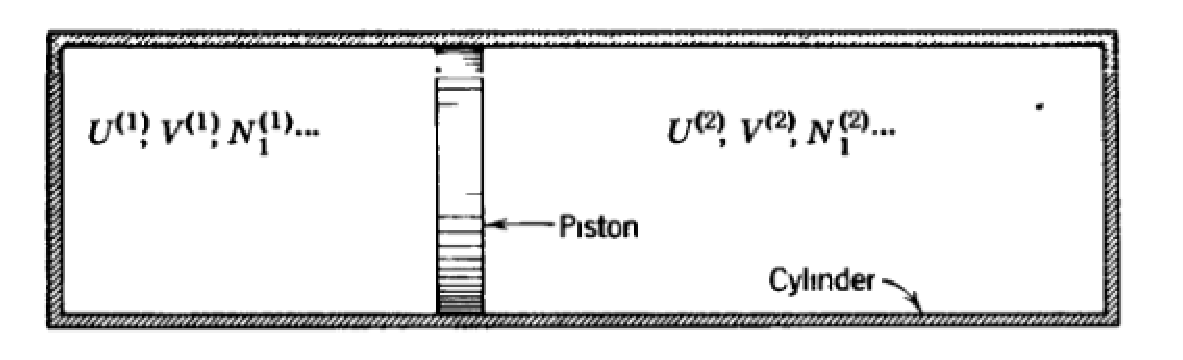
\includegraphics[scale=0.7]{fig1_2.eps}
	\figcaption{}
}}

在下一节讲述解决此问题的定量方法之前,我们用更一般的方式重述基本问题,无需借助气缸与活塞。给定两个或多个简单系统,它们整体可以视为一个{\it 复合 (composite)}系统。封闭的复合系统被限制总能量、总体积与总摩尔数的壁{\it 包围},而封闭复合系统的简单子系统无需是封闭的,比如复合系统内部的活塞可以透热或者有个洞。复合系统的{\it 内部 (internal)}限制阻止了各简单系统之间的能量、体积或物质重新分布。一个封闭的复合系统在某一内部限制下达到平衡态,若将该内部限制去掉,则之前禁止的某些状态现在可能达到。这一过程使系统达到新平衡态。热力学的基本问题就是预言这一新平衡态。

\section{最大熵假设}
\label{sec1.10}
由热力学的中心原理出发可解决热力学基本问题,而从实验观测归纳出中心原理的过程相当微妙。这一人类智慧的杰作在历史上最终由Caratheodory分析完成。以Josiah Willard Gibbs为先驱的统计力学方法需要熟练的归纳性灵感。The symmetry-based foundations to be developed in Chapter 21 will provide retrospective understanding and interpretation, but they are not yet formulated as a deductive basis. 
因此我们仅仅将热力学基本问题的解决方法以一系列后验性的\mpar{意思是假设的正确性由它导出的结论的正确性(后验性地)验证。}假设给出,而非以先验的证据的形式。实际上在考虑到基本问题{\it 最简单的形式解}之后,这些假设是非常自然的。On this basis alone the problem {\it might} have been solved; 将一个问题的最简形式解作为试探性的假设是理论物理学常见而管用的套路。

平衡态最简单而又靠谱的判断标准是什么?物理学的人生经验告诉我们——平衡的黄金准则是让某个量取极值。亦即,我们猜想,处于平衡终态系统的各广延量($U, V, N, \dots$)使得某个函数取最大值\footnote{其实取最小值也可以,假设取最大值只是惯例,两个选项只差一个负号,不影响理论的逻辑结构。}。再(乐观地)假设这个函数有非常好的数学性质\mpar{数学家眼中搞物理的耍流氓系列},这样能保证所导出的理论的简洁性。如前述,下面提出一系列(三个,\ref{sec1.5}节还有一个)假设以解决热力学基本问题。

{\bf 假设 \uppercase\expandafter{\romannumeral2}. } {\it 任意复合系统的平衡态都存在一个广延量的函数(称为熵,记作$S = S(U, V, N_1, \dots, N_r)$),熵在系统处于任意平衡态时定义为有如下性质:

在系统的广延量没有内部限制时,平衡态对应的广延量使得熵函数取最大值。}


{原文:{\it There exists a function (called the entropy S) of the extensive parameters of any composite system, defined for all equilibrium states and 
having the following property: The values assumed by the extensive parameters in the absence of an internal constraint are those that maximize the entropy over the manifold of constrained equilibrium states. }}

必须强调,上面的假设只定义了熵在系统处于平衡态的性质,丝毫未涉及非平衡态。没有内部限制的系统可以处于任何状态,而{\it 其中每个状态都可以当存在某些限制时达到}。这种有限制的平衡态的熵在上面已经被定义,且其中某一平衡态的熵最大。在没有限制的情况下,系统的平衡态就是该最大熵对应的平衡态。

设想两个被透热壁分隔的子系统,总能量$U$在两个子系统之间如何分配?首先考虑将透热壁换为绝热壁的复合系统,子系统的能量分别为$U^{(1)}, U^{(2)}$(当然$U^{(1)} + U^{(2)} = U$)。每个有限制的平衡态\mpar{也许指复合系统的总能量$U$被限制。}$(U^{(1)}, U^{(2)})$对应一个熵,熵在某个特定的$U^{(1)*}, U^{(2)*}$处取最大值。因此当绝热的限制去掉,即子系统由透热壁分隔时,复合系统的平衡态对应的能量分配为$U^{(1)*}, U^{(2)*}$。

热力学的所有问题都可以从\ref{sec1.9}节介绍的基本问题导出。若系统的熵关于广延量的函数关系已知,则基本问题就可迎刃而解。熵关于广延量的函数关系式称为{\it 热力学基本关系 (fundamental relation)}。因此{\it 若系统的基本关系已知,则该系统所有热力学信息都可从中得出}。

上文陈述的内容极其重要。基本关系包含了系统所有的热力学信息——它等价于系统所有的数据、图表等任何描述热力学性质的内容。若系统的基本关系已知,则任何热力学性质都可精确求出。


{\bf 假设 \uppercase\expandafter{\romannumeral3}. } {\it 
复合系统的熵等于所有子系统的熵之和,即熵具有可加性。

熵是连续、可微,且关于内能单调递增的函数。}

由该假设立即可导出一些熵的数学性质。熵具有可加性,即复合系统的熵$S$是各子系统的熵$S^{(\alpha)}$之和:
\begin{equation}
\label{equ1.4}
	S = \sum_\alpha S^{(\alpha)}.
\end{equation}
每个子系统的熵是各自的广延量的函数:
\begin{equation}
\label{equ1.5}
	S^{(\alpha)} = S^{(\alpha)} \Big( U^{(\alpha)}, V^{(\alpha)}, N_1^{(\alpha)}, \dots, N_r^{(\alpha)} \Big).
\end{equation}
将可加性应用于空间上分开的几个子系统,可得熵的如下性质:{\it 简单系统的熵是广延量的一阶齐次函数}。也就是说,将系统的所有广延量变为$\lambda$倍,则熵也变为$\lambda$倍,用公式表示为:
\begin{equation}
\label{equ1.6}
	S(\lambda U, \lambda V, \lambda N_1, \dots, \lambda N_r) = \lambda S(U, V, N_1, \dots, N_r).
\end{equation}

熵关于内能单调递增意味着偏导数大于零:
\begin{equation}
\label{equ1.7}
	\left( \frac{\partial S}{\partial U} \right)_{V, N_1, \dots, N_r} > 0.
\end{equation}
下一章会看到,上式左侧的倒数即为温度$T$的定义,因此根据该假设,温度是非负的\footnote{这个偏导数为负数(即温度为负数)可能性的讨论可见N F Ramsey, {\it Phys. Rev.} 103, 20 (1956). 负温度的真实系统并非处于平衡态,因此与\eqref{equ1.7}式不矛盾。这种状态只能在非常特殊的系统(例如孤立自旋系统)中实现,并且很快就衰变掉了。然而这种负温度状态的研究具有统计力学意义,例如阐明统计力学中温度的概念。 }。

熵的连续、可微性以及关于内能的单调性意味着熵函数可以转化为内能关于$S, V, N_1, \dots, N_r$的{\it 单值、连续以及可微的}函数,即:
\begin{equation}
\label{equ1.8}
	S = S(U, V, N_1, \dots, N_r)
\end{equation}
可以唯一地解出具有如下形式的内能函数$U$:
\begin{equation}
\label{equ1.9}
	U = U(S, V, N_1, \dots, N_r).
\end{equation}
\eqref{equ1.8}与\eqref{equ1.9}式是基本关系的两种形式,它们中的每一个都包含了系统的{\it 所有}热力学信息。

熵的广延性表明$N$摩尔物质的系统的熵等于$1$摩尔系统的熵的$N$倍,这用基本关系表示为:
\begin{equation}
\label{equ1.10}
	S(U, V, N_1, \dots, N_r) = N\, S \left( \frac{U}{N}, \frac{V}{N}, \frac{N_1}{N}, \dots, \frac{N_r}{N} \right).
\end{equation}
上式即为\eqref{equ1.6}式中的因子$\lambda$取$1/N \equiv 1 / \sum_k N_k$的结果。对于单一组分的简单系统有:
\begin{equation}
\label{equ1.11}
	S(U, V, N) = N\, S \left( \frac{U}{N}, \frac{V}{N}, 1 \right),
\end{equation}
$U/N$是单位摩尔数的内能,将它记作$u$:
\begin{equation}
\label{equ1.12}
	u \equiv \frac{U}{N},
\end{equation}
同样,单位摩尔数对应的体积$V/N$记作$v$:
\begin{equation}
\label{equ1.13}
	v \equiv \frac{V}{N}.
\end{equation}
因此$S(U/N, V/N, 1) \equiv S(u, v, 1)$是单位摩尔粒子数的系统的熵,记作$s(u, v)$:
\begin{equation}
\label{equ1.14}
	s(u, v) \equiv S(u, v, 1).
\end{equation}
于是\eqref{equ1.11}式写为
\begin{equation}
\label{equ1.15}
	S(U, V, N) = N s(u, v).
\end{equation}

{\bf 假设 \uppercase\expandafter{\romannumeral4}. } {\it 
在\[ \left( \frac{\partial U}{\partial S} \right)_{V, N_1, \dots, N_r} = 0 \quad \text{(即温度为零)} \]的状态下,任何系统的熵为零。
}

后面会看到,偏导数$(\partial U / \partial S)_{V, N_1, \dots, N_r} = 0$等价于温度$T = 0$。因此假设\uppercase\expandafter{\romannumeral4}的内容是温度为零意味着熵为零。

应该指出,该假设表明熵$S$有确定的零点(就像$V$和$N$那样,而不像$U$)。

假设\uppercase\expandafter{\romannumeral4}是Planck对{\it Nernst 假设}或称为{\it 热力学第三定律}的拓展。它是历史上最晚提出的热力学假设,并且它与经典统计力学不一致,只有在量子统计的框架下才能被接受。大部分热力学内容不需要该假设,我们在第十章才开始用到它。然而它仍然是不可或缺的基本假设之一。

以上所述的四个假设就是建立热力学的逻辑基础。根据这些假设,我们简要地重述\ref{sec1.9}节讲过的热力学基本问题的求解方法。给定一个复合系统,各子系统的基本方程原则上是已知的。子系统处于平衡态时,由基本方程可以算出对应的熵。若复合系统在某些限制下达到平衡态,则每个子系统的广延量会取特定的值以使得总体的熵最大(总熵 = 各子系统熵之和),总系统的熵是各子系统广延量的函数,对基本方程\mpar{熵 = 熵(广延量),即$S = S(U, V, N_1, \dots, N_r)$.}求偏导数以计算熵的极值,再利用二阶偏导将极值点分为极大值、极小值与驻点。在(后文)定义必要的物理概念之后,我们可以将{\it 平衡态}根据{\it 稳定性 (stability)}分类。注意,在引入稳定性的概念后,平衡态的定义会有所变化:上面说的“{\it 平衡态}”今后专指“{\it 稳定平衡态}”\mpar{稳定平衡态对应于熵的极大值点。},而“{\it 不稳定平衡态}”则表示熵函数极大值之外的极值点。

应该指出,尽管所有热力学问题原则上都可以按上述套路求解,但有些情况存在着其他更便利的方法,后面的章节会一一介绍。例如,有时求$U(S, V, N_1, \dots, N_r)$的极小值要比求$S(U, V, N_1, \dots, N_r)$的极大值更简单,这两种方法对应的平衡态是相同的,就像“给定面积的使得周长最小”或“给定周长使得面积最大”所得图形都是圆一样。在后面的章节中我们会引入更多特征函数,将它们极小化等价于将能量极小化或将熵极大化。

基本方程有能量或熵两种形式,极值原理可以是能量取极小值或者熵取极大值,这使得极值假设看起来更加靠谱。在电磁学和力学中,能量是电磁学/力学参数的函数(忽略热效应),平衡条件是能量取极小值。例如一个侧躺的圆锥体比倒放的情况更稳定,因为前者的重力势能更低。考虑热效应之后,能量不仅仅是力学量的函数,然而根据基本方程的变体\mpar{$U = U(S, V, N_1, \dots, N_r)$.},能量的自变量仅仅增加了一个(熵)。将熵引入自变量后最小能量原理就能从力学扩展到热学领域,这样就能得到热力学与力学的对应原理——当热效应可忽略时,热平衡态条件退化到力学平衡条件。

数学告诉我们$S(U, V, N_1, \dots, N_r)$的极大值点对应$U(S, V, N_1, \dots, N_r)$极小值点的条件是$(\partial S/\partial U)_{V, N_1, \dots, N_r} > 0$. 这是引入假设\uppercase\expandafter{\romannumeral3}的动机之一——最大熵原理对应(基本方程为$U(S, V, N, \dots)$的)最小能量原理。

第\uppercase\expandafter{\romannumeral2}部分和第\uppercase\expandafter{\romannumeral3}部分将从对称性根源与统计力学意义上深入探讨熵的概念,但现在就开始的话会脱离正轨。接下来首先要从简单的基本假设出发,导出经典热力学的丰富结论,之后再做深入讨论。


\subsection*{习题}
 

%!TEX root = ../CallenThermo.tex
%----------------------------------------------------------------------------------------
%	翻译:SI
%   校对:lh1962
%----------------------------------------------------------------------------------------

\chapter{平衡条件}
\label{chap2}

\section{强度量}
\label{sec2.1}
基于对过程中广延量相应变化的兴趣,我们希望能对基本方程的微分形式进行研究。将基本方程写为
\begin{equation}
\label{equ2.1}
	U = U(S, V, N_1, \dots, N_r).
\end{equation}
计算一阶微分:
\begin{equation}
\label{equ2.2}
	dU = \left( \frac{\partial U}{\partial S} \right)_{V, N_1, \dots, N_r} dS + \left( \frac{\partial U}{\partial V} \right)_{S, N_1, \dots, N_r} dV + \sum_{j = 1}^r \left( \frac{\partial U}{\partial N_j} \right)_{S, V, \dots, N_r} dN_j.
\end{equation}
上式出现的偏导数十分常用,值得用特定符号标记它们。它们称为{\it 强度量 (intensive parameters)},记作\mpar{这里的“温度”、“压强”、“电化学势”只是起了个名字,但本章后面就会看到这些定义合理之处。}:
\begin{align}
\label{equ2.3}
	\pUpS_{V, N_1, \dots, N_r} &\equiv T, \quad \text{温度} \\
\label{equ2.4}
	-\pUpV_{S, N_1, \dots, N_r} &\equiv P, \quad \text{压强} \\
\label{equ2.5}
	\left( \frac{\partial U}{\partial N_j} \right)_{S, V, \dots, N_k, \dots} &\equiv \mu_j, \quad \text{第j种组分的电化学势}
\end{align}
这样\eqref{equ2.2}式写为
\begin{equation}
\label{equ2.6}
	dU = TdS - PdV + \sum_{j = 1}^r \mu_j dN_j.
\end{equation}
稍后就会看到这样定义的温度与生理上冷热感觉的定性概念相符合,没人愿意采用与经验相冲突的定义。不过现在暂时把温度当做一个数学定义就行了。

类似地,后面会证明这样定义的压强与力学里的压强是一回事。人们一般对电化学势没什么直观印象,因此最后一个定义(\eqref{equ2.5}式)不难接受。

电化学势通常简称为{\it 化学势 (chemical potential)},这两个词语我们都采用\footnote{注意,有些情形(特别是固体理论领域)的“化学势”定义为电化学势$\mu$减去分子静电能量。}。

根据\eqref{equ1.1}式,\eqref{equ2.6}式的$-P dV$项即为(外界对系统做的)准静态功$barta W_M$。

摩尔数不变的情况下,\eqref{equ2.6}式化为
\begin{equation}
\label{equ2.7}
	T dS = dU - \dbar W_M, \quad \text{若}dN_1 = dN_2 = \dots = dN_r = 0.
\end{equation}

利用准静态过程热流的定义\mpar{$\dbar Q \equiv dU - \dbar W.$},或者比较\eqref{equ2.7}式与\eqref{equ1.2}式可得,$TdS$即为准静态热流:
\begin{equation}
\label{equ2.8}
	\dbar Q = TdS.
\end{equation}
{\it 流入系统的准静态热流贡献了其一部分熵增。}

\eqref{equ2.6}式余下的一项与系统加入物质后的内能变化有关。这种能量流动在热力学之外很少讨论(尽管容易想象),因而没有通用的名字。我们称$\sum_j \mu_j dN_j$为{\it 准静态化学功 (quasi-static chemical work)},记作$\dbar W_c$:
\begin{equation}
\label{equ2.9}
	\delta W_c \equiv \sum_{j = 1}^r \mu_j dN_j.
\end{equation}
因此
\begin{equation}
\label{equ2.10}
	dU = \delta Q + \delta W_M + \delta W_c.
\end{equation}
\eqref{equ2.6}式中的每一项——$TdS, -PdV, \mu_j dN_j$都具有能量量纲。\ref{sec2.6}节具体讨论单位的事情。这里应该指出,由于尚未指定熵的量纲与单位,故而温度的量纲仍悬而未决。化学势$\mu$的单位与能量相同(因为粒子数是无量纲的)。根据定义,压强的单位与力学中的一样,不同单位制的转换参见本书封底。

\section{状态方程}
\label{sec2.2}
温度、压强和化学势都是基本方程对自变量$S, V, N_1, \dots, N_r$的偏导数,因此它们也是$S, V, N_1, \dots, N_r$的函数,即
\begin{align}
\label{equ2.11}
	T &= T(S, V, N_1, \dots, N_r) \\
\label{equ2.12}
	P &= P(S, V, N_1, \dots, N_r) \\
\label{equ2.13}
	\mu_j &= \mu_j (S, V, N_1, \dots, N_r)
\end{align}
上面这样将强度量用广延量表示的方程称为{\it 状态方程 (equations of state)}。

单个状态方程{\it 并不}包含系统所有的热力学信息,后面会看到,{\it 全体}状态方程才与基本方程一样完备描述热力学系统。

由基本方程的一阶齐次性可直接导出状态方程是{\it 零阶齐次的 (homogeneous zero order)},也就是说将系统所有广延量变化$\lambda$倍,强度量仍不变:
\begin{align}
	T(\lambda S, \lambda V, \lambda N_1, \dots, N_r) &= \frac{\partial U(\lambda S, \lambda V, \lambda N)}{\partial (\lambda S)} \notag \\
	&= \frac{ \partial \big[ \lambda U(S, V, N) \big] }{\lambda \partial S} \text{(基本方程的一阶齐次性)} \notag \\
	&= \frac{\partial U(S, V, N)}{\partial S} = T(S, V, N) \notag \\
\label{equ2.14}
	T(\lambda S, \lambda V, \lambda N_1, \dots, N_r) &= T(S, V, N_1, \dots, N_r).
\end{align}
可见同一系统部分与整体的温度相等,这符合温度的直观感觉。压强与化学势同样具有\eqref{equ2.14}式的性质。

可以用更简明的符号简化上述式子。将广延量$V, N_1, \dots, N_r$统一记作$X_1, X_2, \dots, X_t$,于是基本方程写为
\begin{equation}
\label{equ2.15}
	U = U(S, X_1, X_2, \dots, X_t).
\end{equation}
强度量为:
\begin{align}
\label{equ2.16}
	\pUpS_{X_1, X_2, \dots, X_t} &\equiv T = T(S, X_1, X_2, \dots, X_t) \\
\label{equ2.17}
	\left( \frac{\partial U}{\partial X_j} \right)_{S, \dots, X_k, \dots} &\equiv P_j = P_j (S, X_1, X_2, \dots, X_t), \quad j = 1, 2, \dots, t.
\end{align}
基本方程的微分形式为
\begin{equation}
\label{equ2.18}
	dU = TdS + \sum_{j = 1}^t P_j dX_j.
\end{equation}
注意\eqref{equ2.4}式有负号,但\eqref{equ2.17}式没有。按照热力学的体系,与强度量$T, \mu_j$地位相同的量是{\it 负压强\mpar{麻烦源于压强$P$是力学中早已定义好了的。} }:$-P$,\eqref{equ2.17}式中某个$P_j$代表的是$-P$.

对于单组分简单系统,各方程经常用单位摩尔数的物理量表示。类似\eqref{equ1.11}与\eqref{equ1.15}式的关系那样,单位摩尔数的内能为
\begin{equation}
\label{equ2.19}
	u = u(s, v),
\end{equation}
其中
\begin{align}
\label{equ2.20}
	s &= \frac{S}{N}, \quad v = \frac{V}{N} \\
\label{equ2.21}
	u(s, v) &= \frac{1}{N} U(S, V, N).
\end{align}
\eqref{equ2.19}式等号两侧微分:
\begin{equation}
\label{equ2.22}
	du = \frac{\partial u}{\partial s} ds + \frac{\partial u}{\partial v} dv,
\end{equation}
再结合
\begin{align}
\label{equ2.23}
	\pups_v &= \pups_{V, N} = \pUpS_{V, N} = T \\
\label{equ2.24}
	\pupv_s &= -P
\end{align}
可得
\begin{equation}
\label{equ2.25}
	du = Tds - Pdv.
\end{equation}

\ 

{\bf \Large 习题}

\ 

\begin{enumerate}
	\item[2.2-1]
		某系统的基本方程为
		\[
			U = \left( \frac{v_0 \theta}{R^2} \right) \frac{S^3}{NV}.
		\]
		(括号里的一坨都是常数,下同)

		求相应的三个状态方程,并验证它们是零阶齐次的。
	\item[2.2-2]
		条件同2.2-1题,用$T, V, N$表示$\mu$.
	\item[2.2-3]
		画出2.2-1题的系统在恒温条件下压强关于体积的变化曲线(等温线)。画两条温度不同的等温线,指出哪一条温度更高。
	\item[2.2-4]
		某系统的基本方程为
		\[
			u = \left( \frac{\theta}{R} \right) s^2 - \left( \frac{R\theta}{v_0^2} \right) v^2,
		\]
		求三个状态方程,并证明对于该系统有$\mu = -u$.
	\item[2.2-5]
		条件同2.2-4问,求$\mu$关于$T, P$的函数关系。
	\item[2.2-6]
		某系统的基本方程为
		\[
			u = \left( \frac{v_0 \theta}{R} \right) \frac{s^2}{v} \mathrm{e}^{s/R}.
		\]
		求三个状态方程。
	\item[2.2-7]
		观测到某系统具有如下关系:
		\[
			u = Av^{-2} e^{s/R}.
		\]
		$N$摩尔该物质组成的系统,初始温度$T_0$,初始压强$P_0$,经历等熵膨胀($S = \text{常数}$)过程,终态压强为$P_0 / 2$,求终态的温度$T_f$。
		\begin{flushright}
			{\it 答案: }$T_f = 2^{-2/3} T_0 = 0.63 T_0.$
		\end{flushright}

		{\it 解:
			\begin{align*}
				U &= Nu = NAv^{-2} \mathrm{e}^{s/R} \\
				&= A \frac{N^3}{V^2} \mathrm{e}^{S/(NR)} \\
				P &= -\pUpV_{S, N} = 2AN^3 \frac{1}{V^3} \mathrm{e}^{S / (NR)}.
			\end{align*}
			等熵膨胀过程初末状态的熵相等:$S_f = S_0 \equiv S$.

			由已知条件$P_f = \frac{1}{2} P_0$, 联立得
			\begin{align*}
				2AN^3 \frac{1}{V_f^3} \mathrm{e}^{S  /(NR)} &= \frac{1}{2} \left( 2AN^3 \frac{1}{V_0^3} \mathrm{e}^{S / (NR)} \right) \\
				\to V_f &= 2^{\frac{1}{3}} V_0. \\
				T &= \pUpS_{V, N} = \frac{A N^2}{R V^2} \mathrm{e}^{S / NR} \\
				T_f &= \frac{A N^2}{R V_f^2} \mathrm{e}^{S / (NR)} \\
				&= \frac{A N^2}{R V_0^2} \mathrm{e}^{S / (NR)} \frac{1}{2^{2/3}} \quad(V_f = 2^{1/3} V_0) \\
				&= 2^{-2/3} T_0 = 0.63 T_0.
			\end{align*}
		}
		\item[2.2-8]
			类似\eqref{equ2.25}式,证明由$r$种组分组成的系统满足:
			\[
				du = Tds - Pdv + \sum_{j = 1}^{r - 1} (\mu_j - \mu_r) dx_j.
			\]
			其中$x_j \equiv N_j / N$,是第$j$种组分的摩尔分数。
		\item[2.2-9]
			某单组分系统在绝热过程中满足$PV^k = \mathrm{constant}$, 其中$k$为正的常数,求证系统的内能为:
			\[
				U = \frac{1}{k - 1} PV + Nf(PV^k / N^k).
			\]
			其中$f$为任意函数。

			{\it 提示:} 由条件知$PV^k$是$S$的函数,且$(\partial U / \partial V)_S = g(S) V^{-k}$, 其中$g(S)$是任意函数。	
\end{enumerate}

\section{熵表象下的强度量}
\label{sec2.3}
前两节的基本方程形式为$U = U(S, \dots, X_j, \dots)$,内能$U$是因变量。基本方程还有另一种以熵$S$为因变量的形式,可以按照与前面相似的步骤建立另一种形式,将$U$记作$X_0$,基本方程写为
\begin{equation}
\label{equ2.26}
	S = S(X_0, X_1, \dots, X_t).
\end{equation}
上式取微分:
\begin{equation}
\label{equ2.27}
	dS = \sum_{k = 0}^t \frac{\partial S}{\partial X_k} dX_k.
\end{equation}
偏导数$\partial S / \partial X_k$记作$F_k$:
\begin{equation}
\label{equ2.28}
	F_k \equiv \frac{\partial S}{\partial X_k}.
\end{equation}
$F_k$与\eqref{equ2.16}、\eqref{equ2.17}式定义的偏导数$P_j$当然有关系,具体为:
\begin{equation}
\label{equ2.29}
	F_0 = \frac{1}{T}, \quad F_k = \frac{-P_k}{T} \quad (k = 1, 2, \dots)
\end{equation}
读者在辨明求偏导数过程中哪些变量保持不变之后不难证明上式,相关的微积分内容可参见附录A。上式也可通过将\eqref{equ2.18}式变形为$dS$的显式形式进而比较得出。

尽管$F_k$与$P_k$关系密切,但原则上它们是截然不同的。$P_k$是微分一个关于$S, \dots, X_j, \dots$的函数得到的,因而$P_k$是$S, \dots, X_j, \dots$的函数。同理,$F_k$是$U, \dots, X_j, \dots$的函数。前一种情况里熵$S$是独立变量中的一个,后者当中内能$U$是独立变量。在热力学的推导/计算过程中必须明确选定其中一种独立变量的集合,并且从一而终不能改变。同一问题混用两套独立变量是许多疑难的万恶之源。

如果选择熵$S$为因变量,因而内能为独立变量,基本方程为$S = S(U, \dots, X_k, \dots)$,则称为在{\it 熵表象 (entropy representation)}下分析问题。如果选择能量为因变量,熵为独立变量,基本方程$U = U(S, \dots, X_k, \dots)$,则称为在{\it 能量表象 (energy representation)}下分析。

热力学的标准理论在两种表象下都可以建立,但特定问题在某一表象下可能大大简化。因此我们平行发展两套表象理论,而且在一种表象下详细讨论之后,转化到另一套表象是比较容易的。

\begin{itemize}
\item 关系式$S = S(X_0, \dots, X_j, \dots)$称为{\it 熵的热力学基本关系 (entropic fundamental relation)},
\item 独立变量集合$X_0, \dots, X_j, \dots$称为{\it 熵的广延量 (entropic extensive parameters)},
\item $F_0, \dots, F_j, \dots$称为{\it 熵的强度量 (entropic intensive parameters)}。
\end{itemize}

类似地,

\begin{itemize}
\item 关系式$U = U(S, X_1, \dots, X_, \dots)$称为{\it 能量的热力学基本关系 (energetic fundamental relation)}, 
\item $S, X_1, \dots, X_, \dots$称为{\it 能量的广延量 (energetic extensive parameters)},
\item $T, P_1, \dots, P_j, \dots$称为{\it 能量的强度量 (energetic intensive  parameters)}。
\end{itemize}

\ 

{\large \bf 习题}

\ 

\begin{enumerate}
	\item[2.3-1.]
		某系统的基本方程为
		\[
			u = \left( \frac{v_0^{1/2} \theta}{R^{3/2}} \right) \frac{s^{5/2}}{v^{1/2}}.
		\]
		求熵表象下的三个状态方程。
		
		\begin{flushright}
		{\it 答案}
		
		$\displaystyle{
			\frac{1}{T} = \frac{2}{5} \left( \frac{v_0^{1/2} \theta}{R^{3/2}} \right)^{-2/5} \frac{v^{1/5}}{u^{3/5}} }$
		
		\ 

		$\displaystyle{
			\frac{\mu}{T} = -\frac{2}{5} \left( \frac{v_0^{1/2} \theta}{R^{3/2}} \right)^{-2/5} u^{2/5} v^{1/5}
		}$		
		\end{flushright}
	\item[2.3-2.]
		作出压强恒定条件下温度随体积的关系曲线(等压线),画出两条压强不同的等压线,指出哪条的压强更大。
	\item[2.3-3.]
		某系统的基本方程为
		\[ 
			u = \left( \frac{\theta}{R} \right) s^2 \mathrm{e}^{-v^2 / v_0^2}
		\]
		求熵表象下的三个状态方程。
	\item[2.3-4.]
		某系统的基本方程为
		\[
			S = AU^n V^m N^r
		\]
		其中$A$是正的常数。热力学基本假设要求$n, m, r$必须满足什么条件?如果要求在$N$一定的条件下$P$关于$U/V$单调递增(这个条件是稳定性条件的要求,见第8章),则$n, m, r$必须满足什么条件?明确起见,能量的零点规定在零温状态。
	\item[2.3-5.]
		某系统的基本方程为
		\[
			\frac{S}{R} = \frac{UV}{N} - \frac{N^3}{UV}.
		\]
		\begin{enumerate}
		\item[(a)]
			验证熵表象下的三个状态方程是零阶齐次的。
		\item[(b)]
			求证温度是正的。
		\item[(c)]
			求“力学状态方程”$P = P(T, v)$.
		\item[(d)]
			求$P-v$平面上绝热线(即等熵线)的形式。
		\end{enumerate}
\end{enumerate}

\section{热平衡态——温度}
\label{sec2.4}
下面讨论关于熵的极值原理的一些有趣的应用。考虑一个封闭的简单复合系统,它的两个子系统由固定且不可透过物质的透热壁分隔,因此子系统的体积与摩尔数恒定,但内能$U^{(1)}, U^{(2)}$可变,复合系统的封闭性要求
\begin{equation}
\label{equ2.30}
	U^{(1)} + U^{(2)} = \text{常数}.
\end{equation}
如何求出平衡状态下子系统的内能$U^{(1)}, U^{(2)}$?根据基本假设,平衡态对应的$U^{(1)}, U^{(2)}$使复合系统的熵取极大值\mpar{一直以来原文采用的都是maximize(最大化),但使用的数学条件是极大值条件$dS = 0, d^2 S < 0$. 因此这里译作极大值。}。根据极值条件,平衡状态下子系统之间无穷小的能量传递不改变复合系统的熵,即
\begin{equation}
\label{equ2.31}
	dS = 0.
\end{equation}
由熵的可加性,复合系统的熵即为两个子系统熵之和:
\begin{equation}
\label{equ2.32}
	S = S^{(1)} (U^{(1)}, V^{(1)}, \dots, N_j^{(1)}, \dots) + S^{(2)} (U{(2)}, V^{(2)}, \dots, N_j^{(2)}, \dots).
\end{equation}
$U^{(1)}, U^{(2)}$的微小变化造成熵的变化为
\begin{equation}
\label{equ2.33}
	dS = \left( \frac{\partial S^{(1)} }{\partial U^{(1)} } \right)_{V^{(1)}, \dots, N_j^{(1)}, \dots} dU^{(1)} + \left( \frac{\partial S^{(2)} }{\partial U^{(2)} } \right)_{V^{(2)}, \dots, N_j^{(2)}, \dots} dU^{(2)}
\end{equation}
利用温度的定义,上式化为
\begin{equation}
\label{equ2.34}
	dS = \frac{1}{T^{(1)}} dU^{(1)} + \frac{1}{T^{(2)}} dU^{(2)}.
\end{equation}
由能量守恒(\eqref{equ2.30}式)可得
\begin{equation}
\label{equ2.35}
	dU^{(2)} = -dU^{(1)}.
\end{equation}
故而
\begin{equation}
\label{equ2.36}
	dS = \left( \frac{1}{T^{(1)}} - \frac{1}{T^{(2)}} \right) dU^{(1)}.
\end{equation}
平衡条件\eqref{equ2.31}式要求$dU^{(1)}$取任意值都有$dS = 0$,因此
\begin{equation}
\label{equ2.37}
	\frac{1}{T^{(1)}} = \frac{1}{T^{(2)}}.
\end{equation}
这就是平衡态条件。如果各子系统的基本方程已知,则$1 / T^{(1)}$是关于$U^{(1)}$的已知函数\mpar{当然还有$V^{(1)}, N_k^{(1)}, \dots$,不过它们都是常数。},同样,$1 / T^{(2)}$也是$U^{(2)}$的已知函数。方程$1 / T^{(1)} = 1 / T^{(2)}$是关于$U^{(1)}, U^{(2)}$的等式。守恒条件$U^{(1)} + U^{(2)} = \text{常数}$提供第二个等式,这样$U^{(1)}, U^{(2)}$原则上即可解出。给出基本方程的特定形式后就能解出$U^{(1)}, U^{(2)}$的值。在实际应用中系统的基本方程可以通过经验观测(测量方式见后文)或者统计力学模型导出。这样热力学理论就能给出确定的定量预言。

\eqref{equ2.37}式可以写为$T^{(1)} = T^{(2)}$,前面将它写成$1 /T^{(1)} = 1 / T^{(2)}$是为了强调分析过程是在熵表象下进行的\mpar{能量$U$作为独立变量之一。},$1 / T^{(1)}$意味着它是$U^{(1)}, V^{(1)}, \dots$的函数,而$T^{(1)}$是$S^{(1)}, V^{(1)}, \dots$的函数。不过\eqref{equ2.37}式的{\it 物理意义}仍然是两个子系统在平衡态下的温度相等。

这个问题的二阶内容是研究平衡态的稳定性。上面的平衡态只利用了极值条件$dS = 0$,但基本假设的内容是熵取极大值。极大值的条件除了$dS = 0$之外还有
\begin{equation}
\label{equ2.38}
	d^2 S < 0.
\end{equation}
这一条件与平衡态的稳定性有关,具体内容在第8章讨论。

\section{温度定义与直观概念的一致性}
\label{sec2.5}
上一节的例子表明两个由透热壁分隔的系统达到平衡态时它们的温度相等,这是温度的定义与直观概念相符合的几个证据之一。

进一步考虑上面的例子。假设初始时两个被绝热壁分隔的子系统有微小的温度差,不妨设
\begin{equation}
\label{equ2.39}
	T^{(1)}_0 > T^{(2)}_0.
\end{equation}
由绝热壁的限制,初始时系统处于平衡态。移除内部的绝热壁限制后系统不再是平衡态,子系统之间有热量流动,复合系统的熵{\it 增加}。系统最终的平衡态为$T^{(1)} = T^{(2)}$,或者复合系统的熵取(相应限制之下的)极大值。末态与初态熵的差值记作$\Delta S$,则 
\begin{equation}
\label{equ2.40}
	\Delta S > 0.
\end{equation}
但是根据\eqref{equ2.36}式,
\begin{equation}
\label{equ2.41}
	\Delta S \approx \left( \frac{1}{T^{(1)}_0 } - \frac{1}{T^{(2)}_0 } \right) \Delta U^{(1)}.
\end{equation}
其中$T^{(1)}_0, T^{(2)}_0$是温度的初始值。根据条件$T^{(1)}_0 > T^{(2)}_0$可得
\begin{equation}
\label{equ2.42}
	\Delta U^{(1)} < 0.
\end{equation}
这意味着热量{\it 从}系统1传递{\it 到}系统2。由此推论热量{\it 从}温度{\it 高}的系统流{\it 向}温度{\it 低}的系统。这再次与温度的直观概念相符。应该注意,这个结论不依赖于$T^{(1)}, T^{(2)}$相差很小的假设,这个假设只是为了计算简明,一般情况进行积分即可。

基于生理学冷热的温度的直观概念有两个基本特征。第一,温度是强度量,系统部分与整体的温度相等。第二,热量从高温系统向低温系统传递。这些特征要求平衡状态下温度相等且具有均匀性。温度的定量定义符合上述要求。


\section{温度单位}
\label{sec2.6}
温度的单位是能量单位除以熵的单位,熵的单位尚未指定,实际上熵的单位怎样都可以。因为熵乘以任意有量纲常量所得具有新量纲的函数满足同样的极值原理——因此与熵等价。为了消除这个任意性,我们指定熵是无量纲的\mpar{从后面的统计力学的角度可见这个选择非常具有物理意义。}。因而温度的量纲与能量相同。注意,就像力矩和功量纲相同但性质不同、单位也不同\mpar{力矩:牛顿·米 (\si{\newton\meter}),功:焦 (\si{\joule})}那样,温度与能量也要清楚区分。能量与温度的{\it 量纲 (dimensions)}都是$[\text{质量} \cdot (\text{长度})^2 / (\text{时间})^2].$能量的{\it 单位 (units)}是焦耳、尔格和卡路里什么的。温度的单位下面讨论%
\mpar{需要注意的是,对物理量量纲和单位的理解并不是唯一的。另一种常见的理解是,单位只是用以描述具有某种量纲的物理量时所必须的一个结构原件,即“数-单位”,并不承载其所描述的物理量的具体性质。具有相同量纲的单位一定可以相互替代,比如文中提到的\si{\newton\meter}和\si{\joule},或\si{\joule}和\si{\kelvin}。}%
。

第4章会介绍Carnot热机,那里会证明一台与两个热力学系统接触而做功的热机的最大效率由两系统温度的比值完全确定。因此{\it 热力学理论提供了测量任意两个热力学系统温度比值的实验方法}。

二系统温度{\it 比值}的可测量性有许多直接推论。首先温度的零点是唯一确定的,不能任意钦点或“移动”。其次,我们可以自由地指定{\it 任一}状态的能量为某个定值,然后其它所有状态的温度都因之确定下来。

同样,温度的计量标准(简称温标,就是温度单位)在指定参考系统某一标准状态的温度之后就完全确定。

不同标准状态的不同钦点温度造成了不同的热力学温标,但是所有热力学温标在$T = 0$处都是一致的。此外,根据\eqref{equ1.7}式,系统的温度不能低于$0$。热力学温度内禀的非负性与所有观测高度一致。

国际单位制(Système International (SI) system)中的温标为Kelvin温标,指定纯水、冰与水蒸气的三相平衡态的温度为$273.16$,该参考状态称为“三相点(triple points)”。相应的温度单位称为kelvin,记作$\si{\kelvin}$.

同一量纲的两个单位——kelvin与joule(焦耳)之间的比值为\SI{1.3806e-23}{\joule\per\kelvin}. 这个比值称为Boltzmann常数,记作$k_\text{B}$,因此$k_\text{B} T$是一个能量值。

Rankine 温标将水的三相点温度钦点为$\frac{9}{5} \times 273.16 = \SI{491.688}{\degreeR}$。Kelvin温度乘以$\frac{9}{5}$就等于Rankine温度。

实际应用的“{\it 国际Kelvin温标}”与上文的“绝对”Kelvin温标关系密切,国际Kelvin温标在不同的温度范围利用特定系统分别进行定义,并且保证与(绝对)Kelvin温标尽量接近。它的优点是提供了不同温度区间内可重复的温度测量实验标准。然而从热力学观点看,它并非真实的热力学温标,因为它与Kelvin温标稍有偏差,使得温度之比不符合热力学理论。

日常生活中的温度无论用Kelvin还是Rankine温标表示数值都很大。例如室温大约是\SI{300}{\kelvin}或\SI{540}{\degreeR}. 因此为了方便,人们又定义了两种衍生温标。Celsius温标\mpar{通常译为摄氏温标,本文统一采用英文名称。}定义为
\begin{equation}
\label{equ2.43}
	T(\si{\degreeCelsius}) = T(K) - 273.15.
\end{equation}
其中$T(\si{\degreeCelsius})$称为“Celsius温度”\mpar{通常译为摄氏温度。},单位称为“{\it Celsius度} (摄氏度)”,记作(\si{\degreeCelsius}. Celsius温标的零点不同于热力学温度的零点,因此{\it Celsius温标绝不是热力学温标}。存在零下的Celsius温度,零Celsius度可以达到,Celsius温度的比值不符合热力学理论。只有Celsius温度差才有热力学意义。

根据定义,水的三相点(冰、水及水蒸气混合物处于平衡态)的“温度”为\SI{0.01}{\degreeCelsius}。压强保持\SI{1}{atm}不变的冰水混合物系统温度更接近\SI{0}{\degreeCelsius},小数点后第三位才非零。\SI{1}{atm}下沸腾的水温度非常接近\SI{100}{\degreeCelsius}. 这两个巧合源自Celsius温标的历史进程\footnote{这方面的历史可见E. R. Jones, Jr., The Physics Teacher 18, 594 (1980). }。在意识到温度的零点唯一之前,人们确定温标需要指定两个特定温度(而非一个)%
\mpar{这个断言并不完整。为了准确测定温度,我们不止需要指定温度的特殊点,还需要指定测温物质和测温属性。例如,单纯利用物体的热膨胀测温,那么水银温度计和酒精温度计将会给出不同的温度结果。而热力学温标与测温物质无关的特性,使得它在物理中被广泛运用。}%
。Anders Celsius在1742年将\SI{0}{\degreeCelsius},\SI{100}{\degreeCelsius}指定为上述两个状态。

实践中常用的还有Fahrenheit温标\mpar{通译为华氏温标。},定义为
\begin{equation}
\label{equ2.44}
	T(\si{\degreeF}) \equiv T(\si{\degreeR}) - 459.67 = \frac{9}{5} T(\si{\degreeCelsius}) + 32.
\end{equation}
\SI{1}{atm}下冰水混合物的Fahrenheit温度大约是\SI{32}{\degreeF}. \SI{1}{atm}下沸水约为\SI{212}{\degreeF}, 室温在\SI{70}{\degreeF}左右。Fahrenheit温标的“巧合”在于\SI{1}{atm}下冰与盐水混合物为\SI{0}{\degreeF}附近,奶牛的体温(直肠温度)大概是\SI{100}{\degreeF}.

尽管前面已经利用热力学基本关系的偏导数正式定义了温度,我们现在简要回顾引入温度概念的通常方法(由Kelvin和Caratheodory建立)。热流$\dbar Q$按照前面能量守恒的方法定义。考虑一个热力学循环过程,可推断出存在一个将不完整微分$\dbar Q$转换成全微分$dS$的积分因子,记做$1/T$
\begin{equation}
\label{equ2.45}
	dS = \frac{1}{T} \dbar Q.
\end{equation}
从而我们便从{\it Pfaffian 型}微分方程积分因子的存在性引入了温度和熵的概念。


\section{力学平衡}
\label{sec2.7}
本节我们将通过一个更为简单的例子来阐明熵的极值原理的应用。考虑一个封闭的复合系统,它的两个子系统由可移动的透热壁分隔\mpar{如果没有特别说明,本节的壁都是不可透过物质的。},子系统的摩尔数是定值,但各自的内能$U^{(1)}, U^{(2)}$可以改变,系统的封闭性要求
\begin{equation}
\label{equ2.46}
	U^{(1)} + U^{(2)} = \text{常数}.
\end{equation}
体积$V^{(1)}, V^{(2)}$也可变,封闭性也要求
\begin{equation}
\label{equ2.47}
	V^{(1)} + V^{(2)} = \text{常数}.
\end{equation}
熵的极值原理要求无穷小的传热或无穷小的体积改变造成的熵变均为零,即
\begin{equation}
\label{equ2.48}
	dS = 0.
\end{equation}
其中
\begin{equation}
\label{equ2.49}
\begin{split}
	dS =& \left( \frac{ \partial S^{(1)} }{ \partial U^{(1)} } \right)_{ V^{(1)}, \dots, N_k^{(1)}, \dots} dU^{(1)} + \left( \frac{ \partial S^{(1)} }{ \partial V^{(1)} } \right)_{ U^{(1)}, \dots, N_k^{(1)}, \dots} dV^{(1)} \\
	&+ \left( \frac{ \partial S^{(2)} }{ \partial U^{(2)} } \right)_{ V^{(2)}, \dots, N_k^{(2)}, \dots} dU^{(2)} + \left( \frac{ \partial S^{(2)} }{ \partial V^{(2)} } \right)_{ U^{(2)}, \dots, N_k^{(2)}, \dots} dV^{(2)}
\end{split}
\end{equation}
由封闭性条件可得
\begin{align}
\label{equ2.50}
	dU^{(2)} = -dU^{(1)} \\
\label{equ2.51}
	dV^{(2)} = -dV^{(1)}
\end{align}
于是
\begin{equation}
\label{equ2.52}
	dS = \left( \frac{1}{T^{(1)}} - \frac{1}{T^{(2)}} \right) dU^{(1)} + \left( \frac{ P^{(1)} }{ T^{(1)} } - \frac{ P^{(2)} }{ T^{(2)} } \right) dV^{(1)} = 0
\end{equation}
因$dU^{(1)}, dV^{(1)}$任意取值,故而相应系数为零,即
\begin{align}
	\frac{1}{T^{(1)}} - \frac{1}{T^{(2)}} = 0 \label{equ2.53} \\
	\frac{ P^{(1)} }{ T^{(1)} } - \frac{ P^{(2)} }{ T^{(2)} } = 0 \label{equ2.54}
\end{align}
上两式是熵表象下平衡态条件的标准形式,它们可以化为更直接的形式:
\begin{align}
	T^{(1)} = T^{(2)} \label{equ2.55} \\
	P^{(1)} = P^{(2)} \label{equ2.56}
\end{align}
温度相等正是上一节导出的透热壁平衡态的条件。新条件——压强相等对应于壁的可移动特征,压强相等也是力学的平衡条件,由此可见我们定义的压强与力学中压强的一致性。

在熵表象中,$1 / T^{(1)}$是$U^{(1)}, V^{(1)}$的函数\mpar{当然还有摩尔数$N$,不过它们都是常数。}(即熵的状态方程),因此\eqref{equ2.53}式是$U^{(1)}, V^{(1)}, U^{(2)}, V^{(2)}$之间的方程。同样,$P^{(1)} / T^{(1)}$是$U^{(1)}, V^{(1)}$的函数,\eqref{equ2.54}式是$U^{(1)}, V^{(1)}, U^{(2)}, V^{(2)}$之间的方程。 再加上两个守恒方程\eqref{equ2.46}, \eqref{equ2.47}式就构成了四个方程,可以求解四个未知函数$U^{(1)}, V^{(1)}, U^{(2)}, V^{(2)}$. 这就是热力学理论解决这类问题的基本框架,在给定具体的基本方程或状态方程之后即可求解。

子系统由可移动的绝热壁(而非透热壁)分隔的情形十分微妙,我们在进一步学习热力学体系之后再来考虑,习题2.7-3初步介绍了微妙之处,习题5.1-2深入讨论。

\begin{example}


如图,三个圆柱体的横截面积相同,由活塞封印着一定气体(气体的组分不必相同)。活塞通过刚性杠杆连接,它们的“力臂”(即连接点到支点的距离)之比为$1 : 2 : 3$。圆柱体放置在质量可忽略的传热板上,板的唯一作用是使三个圆柱体系统可以传热,其它物理效果可忽略。整个大系统是孤立的,活塞不受外部压强影响。求平衡态下三个圆柱体的压强之比与温度之比。

{
	\centering
	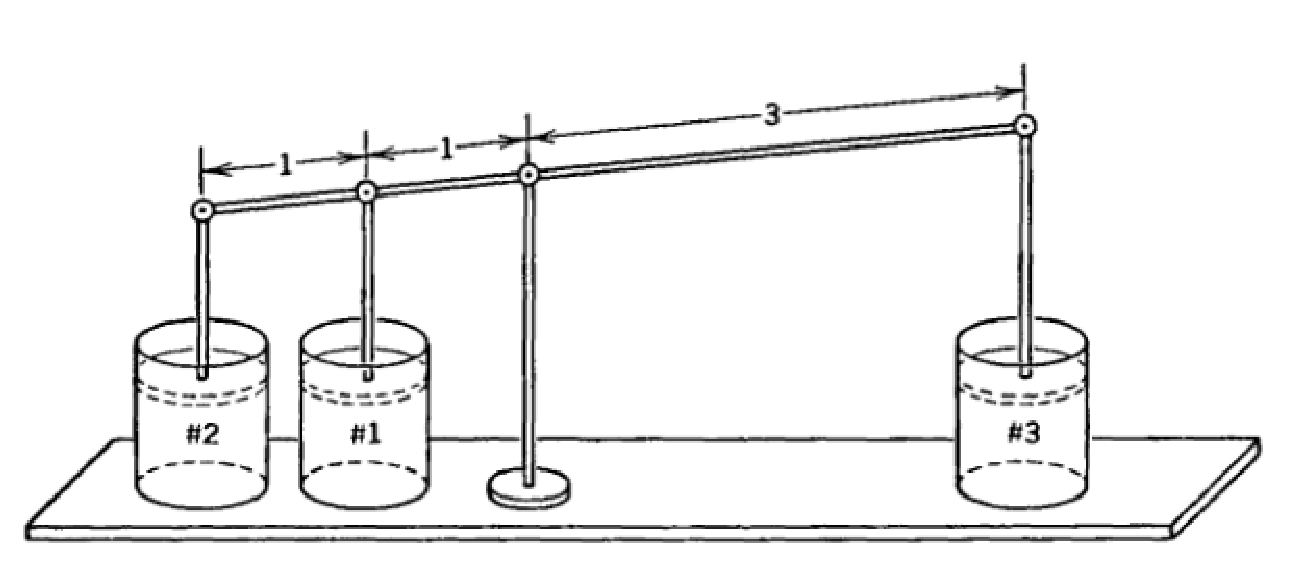
\includegraphics[scale=0.5]{fig2_1.eps} 
	\figcaption{例2.7-1图:三个体积耦合的系统。}
}


{\bf 解}

\ 

{\it 
	封闭性条件要求总能量守恒:
	\[
		\delta U^{(1)} + \delta U^{(2)} + \delta U^{(3)} = 0.
	\]
	活塞之间通过杠杆连接,使得三个圆柱体体积变化的关系为
	\begin{align*}
		\delta V^{(2)} &= 2 \delta V^{(1)} \\
		\delta V^{(3)} &= -3 \delta V^{(1)}
	\end{align*}
	于是熵的极值条件可化为
	\begin{align*}
		\delta S =& \frac{1}{T^{(1)}} \delta U^{(1)} + \frac{1}{T^{(2)}} \delta U^{(2)} + \frac{1}{T^{(3)}} \delta U^{(3)} + \frac{P^{(1)}}{T^{(1)}} \delta V^{(1)} \\
		&+ \frac{P^{(2)}}{T^{(2)}} \delta V^{(2)} + \frac{P^{(3)}}{T^{(3)}} \delta V^{(3)} = 0 \\
		\delta S =& \left( \frac{1}{T^{(1)}} - \frac{1}{T^{(3)}} \right) \delta U^{(1)} + \left( \frac{1}{T^{(2)}} - \frac{1}{T^{(3)}} \right) \delta U^{(2)} \\
		&+ \left( \frac{P^{(1)}}{T^{(1)}} + 2\frac{P^{(2)}}{T^{(2)}} - 3\frac{P^{(3)}}{T^{(3)}} \right) \delta V^{(1)} = 0
	\end{align*}
	$\delta U^{(1)}, \delta U^{(2)}, \delta V^{(1)}$相互独立,可任意取值,因此上式意味着它们的系数均为零。$\delta U^{(1)}$的系数为零可得$T^{(1)} = T^{(3)}$,$\delta U^{(2)}$可得$T^{(2)} = T^{(3)}$,$\delta V^{(1)}$的系数为零结合三个系统温度相等可得
	\[ P^{(1)} + 2P^{(2)} = 3P^{(3)}. \]
	考虑到力学中的杠杆平衡原理,上面的平衡条件在意料之中。若已知状态方程就可将上式化为三个系统体积的等式。
}
\end{example}

\section{存在物质交换时的平衡态}
\label{sec2.8}
化学势的含义要从存在物质流动的情况考虑。设想由不可移动的透热壁分隔的两个简单系统,且第$\alpha$种物质组分\mpar{为避免与子系统编号$\ ^{(1)}, \ ^{(2)}$混淆,本节用希腊字母$\alpha, \beta, \gamma, \dots$标记不同的物质组分,而非采用原书的数字下标。}可以透过壁,其他组分$N_\beta, \dots$不可透过,这个复合系统的平衡态条件是参量$U^{(1)}, U^{(2)}, N_\alpha^{(1)}, N_\alpha^{(2)}$,复合系统熵的微分为
\begin{equation}
	dS = \frac{1}{T^{(1)}} dU^{(1)} - \frac{\mu_\alpha^{(1)}}{T^{(1)}} dN_\alpha^{(1)} + \frac{1}{T^{(2)}} dU^{(2)} - \frac{\mu_\alpha^{(2)}}{T^{(2)}} dN_\alpha^{(2)}
\label{equ2.57}
\end{equation}
封闭性条件为
\begin{align}
	dU^{(2)} &= -dU^{(1)} \label{equ2.58}\\
	dN_\alpha^{(2)} &= - dN_\alpha^{(1)}
\label{equ2.59}
\end{align}
于是
\begin{equation}
	dS = \left( \frac{1}{T^{(1)}} - \frac{1}{T^{(2)}} \right) dU^{(1)} - \left( \frac{\mu_\alpha^{(1)}}{T^{(1)}} - \frac{\mu_\alpha^{(2)}}{T^{(2)}} \right) dN_\alpha^{(1)}.
\label{equ2.60}
\end{equation}
对任意$dU^{(1)}, dN_\alpha^{(1)}$有$dS = 0$,因此平衡条件为
\begin{align}
	\frac{1}{T^{(1)}} = \frac{1}{T^{(2)}} 
\label{equ2.61} \\
	\frac{\mu_\alpha^{(1)}}{T^{(1)}} = \frac{\mu_\alpha^{(2)}}{T^{(2)}}, \quad (\text{因此} \mu_\alpha^{(1)} = \mu_\alpha^{(2)})
\label{equ2.62}
\end{align}
就像温度可以看做热流的“势”,压强为体积变化的“势”那样,化学势可以视为物质流动的“势”。化学势的差值是造成物质流动的“广义力”。

物质流动的方向与化学势的关系可以用\ref{sec2.5}节分析热流的方法导出。设子系统温度相等$T^{(1)} = T^{(2)}$,\eqref{equ2.60}式化为
\begin{equation}
	dS = \frac{\mu_\alpha^{(2)} - \mu_\alpha^{(1)}}{T} dN_\alpha^{(1)}
\label{equ2.63}
\end{equation}
如果$\mu_\alpha^{(1)} > \mu_\alpha^{(2)}$,则由于$dS > 0$, 故而$dN_\alpha^{(1)}< 0$,即物质从高化学势流向低化学势的地方。

之后会看到化学势除了提供物质流动的“广义力”之外,还与物质相变以及化学反应有关,“化学势”的名字正是源自它在理论化学中的重要地位。

化学势的单位是Joule每摩尔(或任意的能量单位每摩尔)。


\section{化学平衡}
\label{sec2.9}
发生化学反应的系统的热力学描述与前面的复合系统相似,它的平衡条件仍然由化学势$\mu$的方程表示——这也是{\it 化学势}名字的来源。

在化学反应过程中,系统物质组分的摩尔数发生变化,有些增加有些减少。摩尔数之间的变化关系由化学反应方程决定,例如
\begin{equation}
	2\ce{H2} + \ce{O2} \leftrightharpoons 2 \ce{H2O}
\label{equ2.64}
\end{equation}
再比如
\begin{equation}
	2\ce{O} \leftrightharpoons \ce{O2}
\label{equ2.65}
\end{equation}
第一个方程里,氢分子、氧分子与水分子变化量之比为$-2 : -1 : +2$. 一般形式是,对于$r$种物质参与的化学反应有:
\begin{equation}
	0 \leftrightharpoons \sum_j \nu_j A_j.
\end{equation}
其中$\nu_j$称为“计量系数 (stoichiometric coefficients)”,例子中氢分子、氧分子与水分子的计量系数分别为$-2, -1, +2$. $A_j$表示化学势,上例中$A_1 = \ce{H2}, A_2 = \ce{O2}, A_3 = \ce{H2O}$. 如果从反方向考虑化学反应(例如水{\it 离解}成氢气氧气),则$\nu_j$反号。$\nu_j$没有绝对的正负性,只有相对的正负才有意义。

系统的基本方程为
\begin{equation}
	S = S(U, V, N_1, N_2, \dots, N_r).
\label{equ2.67}
\end{equation}
假设整个反应体系处于封闭的刚性绝热容器中,系统的总能量$U$,总体积$V$不变。\mpar{这当然不是化学反应最一般的边界条件,一般情况下容器是开放的,可以与外界交换能量,体积也可改变。我们在6.4节讨论这种开放条件下的反应。}

化学反应造成的熵变为
\begin{equation}
	dS = - \sum_{j = 1}^{r} \frac{\mu_j}{T} dN_j.
\label{equ2.68}
\end{equation}
注意,摩尔数的改变与计量系数$\nu_j$成正比,设比例系数为$d\bar{N}$,则
\begin{equation}
	dS = -\frac{d\bar{N}}{T} \sum_{j = 1}^r \mu_j \nu_j
\label{equ2.69}
\end{equation}
因而熵的极值原理表明平衡条件为
\begin{equation}
	\sum_{j = 1}^r \mu_j \nu_j = 0.
\label{equ2.70}
\end{equation}
若系统的状态方程已知,则由平衡条件\eqref{equ2.70}式可以解出平衡状态下各组分的摩尔数。

下面举一个例子。设一个封闭容器内有氢气、氧气与二氧化碳,并进行如下反应:
\begin{equation}
\begin{split}
	\ce{H2} + \frac{1}{2} \ce{O2} &\leftrightharpoons \ce{H2O} \\
	\ce{CO2} + \ce{H2} &\leftrightharpoons \ce{CO} + \ce{H2O} \\
	\ce{CO} + \frac{1}{2} \ce{O2} &\leftrightharpoons \ce{CO2}
\end{split}
\label{equ2.71}
\end{equation}
平衡条件为
\begin{equation}
\begin{split}
	\mu_{\ce{H2}} + \frac{1}{2} \mu_{\ce{O2}} &= \mu_{\ce{H2O}} \\
	\mu_{\ce{CO2}} + \mu_{\ce{H2}} &= \mu_{\ce{CO}} + \mu_{\ce{H2O}} \\
	\mu_{\ce{CO}} + \frac{1}{2} \mu_{\ce{O2}} &= \mu_{\ce{CO2}}
\end{split}
\label{equ2.72}
\end{equation}
上面只有{\it 两个}独立方程(第一个方程是后两个方程的和,第一个化学反应是后两个反应的净结果)。开始反应时氢气、氧气与二氧化碳物质的量之比(可人为控制任意改变)提供另外三个条件。于是有五个未知量(\ce{H2}, \ce{O2}, \ce{H2O}, \ce{CO2}, \ce{CO}的量),五个方程,原则上可以解出。

通常情况在开放容器中的化学反应终态的温度与压强均为定值。因此尽管未知量增加了两个(能量与体积),但$T$与$P$的关系提供了两个新条件,问题同样可以求解。

关于化学反应更详尽的讨论见6.4节。现在只需要记住化学势在物质流动和化学反应中的角色就像温度在热量流动、压强在体积变化中一样。

%!TEX root = ../CallenThermo.tex
%----------------------------------------------------------------------------------------
%	翻译:SI, 哪托儿闹海
%   校对:未校对!
%----------------------------------------------------------------------------------------


\chapter{形式关系与样例系统}
\label{chap3}

\section{热力学Euler方程}
\label{sec3.1}
上一章从基本假设出发解出了平衡态条件,下面深入探究基本方程的数学特征。

基本方程的一阶齐次性使得它可以写成更方便的形式,称为Euler形式。

从一阶齐次性的定义出发,对任意常数$\lambda$都有:
\begin{equation}
\label{equ3.1}
    U(\lambda S, \lambda X_1, \dots, \lambda X_t) = \lambda U(S, X_1, \dots, X_t).
\end{equation}
等式两侧对$\lambda$求导:
\begin{align}
    \frac{ \partial U(\dots, \lambda X_k, \dots)}{\partial (\lambda S)} \frac{\partial (\lambda S)}{\partial \lambda} + \frac{ \partial U(\dots, \lambda X_k, \dots)}{\partial (\lambda X_j)} \frac{\partial (\lambda X_j)}{\partial \lambda} \notag \\
    + \dots = U(S, X_1, \dots, X_t) \label{equ3.2} \\
    \frac{\partial U(\dots, \lambda X_k, \dots)}{\partial (\lambda S)} S + \sum_{j = 1}^t \frac{\partial U(\dots, \lambda X_k, \dots)}{\partial (\lambda X_j)} X_j \notag \\
    = U(S, X_1, \dots, X_t) \label{equ3.3}
\end{align}
方程对任意$\lambda$都成立,取$\lambda = 1$可得:
\begin{align}
    \pUpS S + \sum_{j = 1}^t \frac{\partial U}{\partial X_j} X_j + \dots = U \label{equ3.4} \\
    U = TS + \sum_{j = 1}^t P_j X_j \label{equ3.5}
\end{align}
对于简单系统,上式写为
\begin{equation}
\label{equ3.6}
    U = TS - PV + \mu_1 N_1 + \dots + \mu_r N_r
\end{equation}
\eqref{equ3.5}或\eqref{equ3.6}式是齐次函数Euler定理\mpar{若函数$f(x, y, \dots)$满足$f(\lambda x, \lambda y, \dots) = \lambda^n f(x, y, \dots)$, 则$f$称为$n$阶齐次的。齐次函数Euler定理为$x \frac{\partial f}{\partial x} + y \frac{\partial f}{\partial y} + \dots = n f$.}的一阶齐次情形在热力学理论的应用。公式的推导过程即为齐次定理的证明过程。\eqref{equ3.5}或\eqref{equ3.6}式称为(热力学)Euler关系。

类似地,熵表象下Euler关系的形式为
\begin{align}
    S &= \sum_{j = 0}^t F_j X_j \label{equ3.7} \\
    S &= \left(\frac{1}{T} \right) U + \left( \frac{P}{T} \right) V - \sum_{k = 1}^r \left( \frac{\mu_k}{T} \right) N_k. \label{equ3.8}
\end{align}

\subsection*{习题}
\begin{itemize}
\item[3.1-1.] 写出习题1.10-1当中具有物理意义的基本方程的Euler形式。
\end{itemize}

\section{Gibbs-Duhem关系}
\label{sec3.2}
第二章导出了用温度、压强和化学势表示的平衡条件。这些强度量的引入过程比较相似,事实上,它们的形式体系也是对称的。尽管号称有对称性,但我们对温度与压强有着非常直观的感受,而对化学势就差了一点。有趣的是,这些强度量之间不是完全独立的,它们之间存在函数关系,例如单组分系统的化学势$\mu$可表示为$T, P$的函数。

这种关系是基本方程一阶齐次性的结果。考虑某一单组分系统,基本方程可写为$u = u(s, v)$(即\eqref{equ2.19}式);三个强度量也都是$s, v$的函数,原则上这三个状态方程
\begin{align*}
    T &= T(u, v) \\
    P &= P(u, v) \\
    \mu &= \mu (u, v)
\end{align*}
可消去$u, v$形成一个关于$T, P, \mu$的方程。

容易推广到一般情况,关键还是数清楚变量与方程的数目。设基本方程具有$t + 1$个广延量:
\begin{equation}
\label{equ3.9}
    U = U(S, X_1, X_2, \dots, X_t).
\end{equation}
由此产生$t + 1$个状态方程:
\begin{equation}
\label{equ3.10}
    P_k = P_k(S, X_1, X_2, \dots, X_t).
\end{equation}
令\eqref{equ2.14}式中的任意参量$\lambda$为$\lambda = 1 / X_t$,可得
\begin{equation}
\label{equ3.11}
	P_k = P_k \left( \frac{S}{X_t}, \frac{X_1}{X_t}, \dots, \frac{X_{t-1}}{X_t}, 1 \right).
\end{equation}
可见这$t + 1$个强度量都是关于$t$个变量的函数,从$t + 1$个方程中消去$t$个变量就得到强度量之间的关系。

知道基本方程的具体形式就能求出强度量之间关系的具体形式。给定基本方程之后的套路即为$\eqref{equ3.9} \sim \eqref{equ3.11}$式的过程。

这种关系的微分形式(称为{\bf Gibbs-Duhem关系})可以从Euler关系直接导出。对\eqref{equ3.5}式微分得到
\begin{equation}
\label{equ3.12}
	\,\mathrm dU = T\,\mathrm dS + S\,\mathrm dT + \sum_{j = 1}^t P_j \,\mathrm dX_j + \sum_{j = 1}^t X_j \,\mathrm dP_j.
\end{equation}
由\eqref{equ2.6}式可得
\begin{equation}
\label{equ3.13}
	\,\mathrm dU = T\,\mathrm dS + \sum_{j = 1}^t P_j \,\mathrm dX_j.
\end{equation}
以上两式相减即得到Gibbs-Duhem关系:
\begin{equation}
\label{equ3.14}
	S\,\mathrm dT + \sum_{j = 1}^t X_j \,\mathrm dP_j = 0.
\end{equation}
对于单组分简单系统有
\begin{equation}
\label{equ3.15}
	S\,\mathrm dT - V\,\mathrm dP + N\,\mathrm d\mu = 0.
\end{equation}
或者
\begin{equation}
\label{equ3.16}
	\,\mathrm d\mu = -s\,\mathrm dT + v\,\mathrm dP
\end{equation}
可见化学势的变化与温度及压强的变化有关,而非独立变化,并且$\mu, T, P$三者中已知任何两个的变化就能确定其余一个的变化。

Gibbs-Duhem关系是强度量之间关系的微分形式,将该式积分即得到显式形式,这是除$\eqref{equ3.9} \sim \eqref{equ3.11}$式外的另一种计算套路。Gibbs-Duhem关系的积分:
\[
	\int S(T, P_1, \dots, P_t) \,\mathrm dT + \sum_{j = 1}^t \int X_j(T, P_1, \\,\mathrm dots, P_t) \,\mathrm dP_j = 0
\]
需要知道各广延量$X_j$用强度量$P_j$表示的形式,这可以从状态方程\mpar{状态方程:强度量作为广延量的函数}解出。因此积分Gibbs-Duhem关系必须知道系统的状态方程。

系统可独立变化的强度量个数称为系统的{\it 热力学自由度 (thermodynamic degrees of freedom)}。{\it 一个具有$r$种组分的简单系统的热力学自由度为$r + 1$.}

熵表象下的Gibbs-Duhem关系依旧表示为全体广延量与相应强度量微分之积的和为零:
\begin{align}
	&\sum_{j = 0}^t X_j \,\mathrm dF_j = 0 \label{equ3.17} \\
	&U \,\mathrm d\left( \frac{1}{T} \right) + V \,\mathrm d\left( \frac{P}{T} \right) - \sum_{k = 1}^r N_k \,\mathrm d\left( \frac{\mu_k}{T}\right) = 0 \label{equ3.18}
\end{align}


\subsection*{习题}
\begin{itemize}
\item[3.2-1.] 某系统的基本方程为
\[
	U = \left( \frac{v_0^2 \theta}{R^3} \right) \frac{S^4}{NV^2}
\]
求$T, P, \mu$之间的函数关系。
\end{itemize}

\section{形式关系总结}
\label{sec3.3}
现在总结一下能量表象的热力学体系结构。简明起见,考虑单组分的简单系统,它的基本方程
\begin{equation}
\label{equ3.19}
    U = U(S, V, N)
\end{equation}
包含了该系统所有的热力学信息。定义了温度$T \equiv \partial U / \partial S$等强度量之后,从基本方程可以导出三个状态方程:
\begin{align}
    T &= T(S, V, N) = T(s, v) \label{equ3.20} \\
    P &= P(S, V, N) = S(s, v) \label{equ3.21} \\
    \mu &= \mu(S, V, N) = \mu(s, v) \label{equ3.22}
\end{align}
如果三个状态方程{\it 均}已知,将它们带入Euler关系,即可重新得到基本方程。{\it 因此三个状态方程整体等价于基本方程,}二者都蕴含系统的全部热力学信息,单个的状态方程的热力学信息量少于基本方程。

如果已知两个状态方程,带入Gibbs-Duhem关系再积分即可得到第三个,只是这样得到的状态方程含有一个未定的积分常数。因此两个状态方程(几乎)能够确定基本方程,只差一个未定常数。

当已知两个状态方程时,推导基本方程有更直接、更便利的方法(当然,该方法与利用Gibbs-Duhem关系的途径在逻辑上是等价的):直接积分单位摩尔数的热力学关系:
\begin{equation}
    \,\mathrm du = T\,\mathrm ds - P\,\mathrm dv.
\label{equ3.23}
\end{equation}
将已知的两个状态方程$T = T(s, v), P = P(s, v)$带入上式,即得到$u, s, v$之间的微分方程,再积分就得到
\begin{equation}
    u = u(s, v).
\label{equ3.24}
\end{equation}
这正是基本方程。当然,这个方程里有一个未定的积分常数。

内能总可以表为除了$S, V, N$以外的其它参量的函数。例如$U = U(S, V, N)$与$T = T(S, V, N)$联立消去$S$得到方程$U = U(T, V, N)$. 不过,必须强调的是,这样的方程{\it 并非}基本方程,不包含全部热力学信息。比如,在考虑到$T \equiv \partial U / \partial S$之后,$U = U(T, V, N)$实际上是个偏微分方程。即使它可积,积出的基本方程也带有未定函数。

如果基本方程$U = U(S, V, N)$已知,则相应的$U = U(T, V, N)$唯一确定;但反之不然,确定的$U = U(T, V, N)$并不唯一对应$U = U(S, V, N)$. 它们携带着的都是正确的信息. $U = U(S, V, N)$与$U = U(T, V, N)$都是正确的,但只有前者含有最完整的信息。  

上述内容可以用如下的图例简单说明。设$V, N$不变,内能$U$只随$S$变化,相应的$U\text{-}S$函数图像如图3.1(a)中的实线,这条曲线唯一确定了图3.1(b)所示的$U\text{-}T$曲线,因为$U(S)$每一点都有确定的斜率$T \equiv \partial U / \partial S$, 从而决定了$U(T)$。但如果反过来,已知$U(T)$函数(亦即,一个状态方程),能否决定$U(S)$? 当然不能。 图3.1(a)中的每条虚线之间之差一个“平移”\mpar{这来自求解偏微分方程$U = U(\partial U / \partial S)$留下的“积分常数”。},它们在相同的$U$处的斜率相等,{\it 都能}导出给定的$U(T)$。因此,图3.1(a)可以导出3.1(b),反之则不然。等价的说法是,只有$U = U(S)$才是基本关系。接下来在讨论几个特定的热力学样例系统后,我们将建立正式的理论结构。

{
	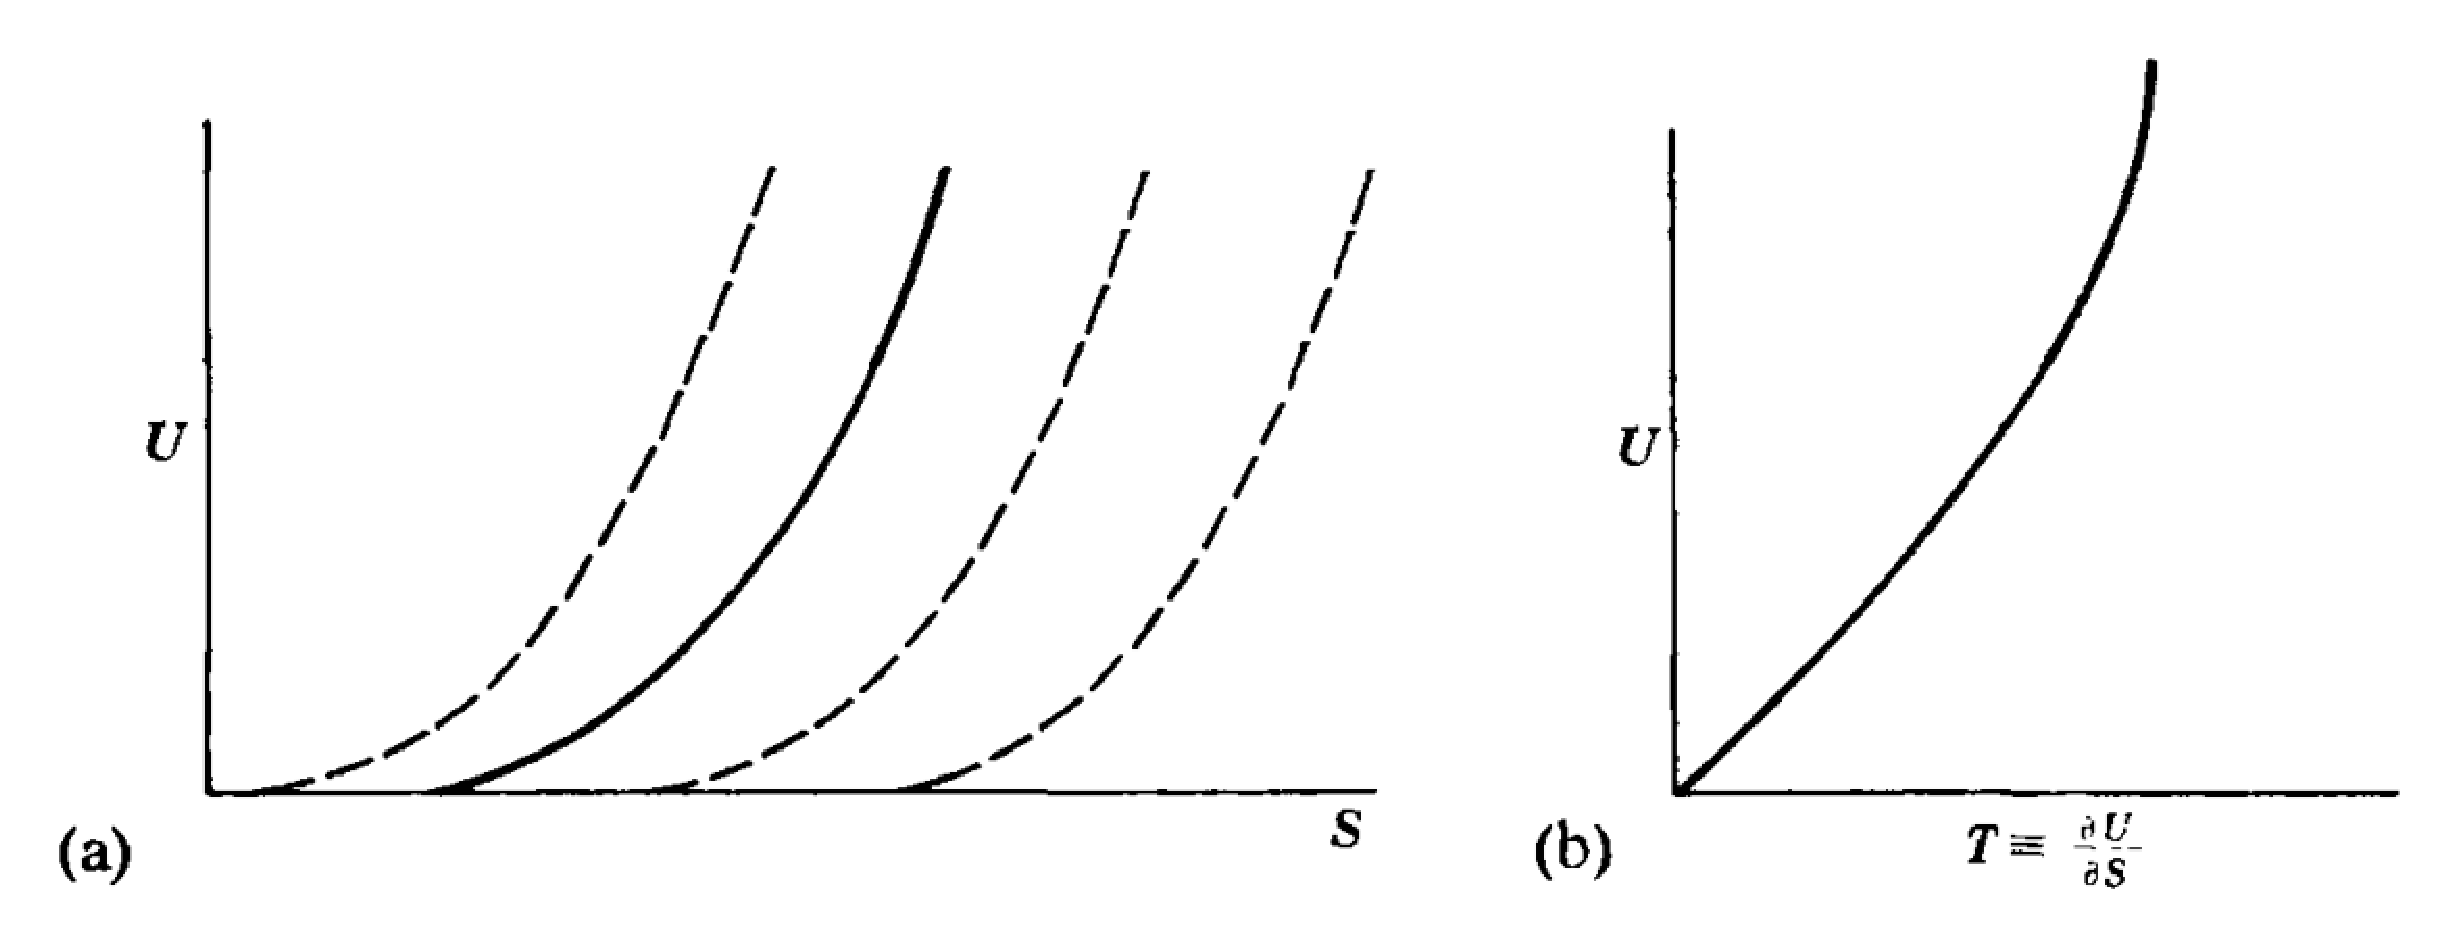
\includegraphics[scale=0.25]{fig3_1.eps} 
	\figcaption{ }
}

\begin{example}

某热力学系统满足条件
\begin{align*}
    U &= \frac{1}{2} PV, \\
    T^2 &= \frac{AU^{3/2}}{VN^{1/2}}.
\end{align*}
其中$A$是大于零的常数。求系统的基本方程。

{\bf 解}

已知条件中出现的独立变量为$U, V, N$,因此采用熵表象求解,首先将这两个已知方程化为熵表象标准形式:
\begin{align*}
    \frac{1}{T} &= A^{-1/2} u^{-3/4} v^{1/2} \\
    \frac{P}{T} &= 2A^{-1/2} u^{1/4} v^{-1/2}
\end{align*}
单位摩尔数基本方程的微分形式(类比\eqref{equ3.23}式)为
\begin{align*}
    ds &= \frac{1}{T} du + \frac{P}{T} dv \\
    &= A^{-1/2} (u^{-3/4} v^{1/2} du + 2u^{1/4} v^{-1/2} dv) \\
    &= 4A^{-1/2} d(u^{1/4} v^{1/2})
\end{align*}
解得
\begin{align*}
    s &= 4A^{-1/2} u^{1/4} v^{1/2} + s_0 \\
    \to S &= 4A^{-1/2} U^{1/4} V^{1/2} N^{1/4} + Ns_0
\end{align*}
当然还有另一种做法:首先对Gibbs-Duhem关系积分从而得到$\mu (u, v)$,然后将所得的三个状态方程带入Euler方程。读者应该尝试一下。

读者还应该注意例题中积分$ds$得到$s$的过程。$ds$关于$du$与$dv$的等式是一个{\it 偏微分方程},它{\it 不能}逐项积分,也不能用求解常微分方程的常用套路。我们通过“观察”对该方程进行积分,“恰好”发现$u^{-3/4} v^{1/2} du + 2u^{1/4} v^{-1/2} dv$正是$d(u^{1/4} v^{1/2})$. \sout{所以老师都不太愿意编习题}

\end{example}

\subsection*{习题}


\section{单组分/多组分简单理想气体}
\label{sec3.4}

单一组分简单理想气体可以用两个方程来描述:
\begin{align}
PV=NRT \label{equ3.25}\\
U=cNRT \label{equ3.26}
\end{align}
其中$c$是常值,$R$是一个普适的气体常数——热力学常数($R=N_Ak_B=8.3144\ \text{J/mole K}$).

上面的是比较理想化的方程。在现实世界中,人们发现,单原子气体(比如Ar、He)有可能符合方程\eqref{equ3.25}\eqref{equ3.26},如果其温度和压力再满足一定要求的话,具体而言,就是$k_BT$相较于电子激发能而言很小(比如当$T\lesssim \SI{e4}{\kelvin}$)而且压强相对较低,那么该气体就会符合上面的两个方程.此外,对所有的这种单原子气体都有$c=\frac{3}{2}$.

在一些更苛刻的条件下,其他的真实气体也有可能满足简单理想气体方程\eqref{equ3.25}\eqref{equ3.26},但是其$c$有可能不再是$3\over2$. 举个例子,双原子气体(比如NO、O$_2$)的$c$在一个很大的温度范围内约为${5\over2}$,在更高的温度下其$c$约为$7\over2$(两种情况的分界温度数量级一般在$10^3K$)。

通过方程\eqref{equ3.25}\eqref{equ3.26}可以确定基本方程. 方程\eqref{equ3.26}中内能$U$的形式很简单,这就启示我们:在熵表象下处理问题可能会更简单。将方程重写为合适的形式:
\begin{align}
\frac{1}{T}=cR\left(\frac{N}{U}\right)=\frac{cR}{u}\label{equ3.27}\\
\frac{P}{T}=R\left(\frac{N}{V}\right)=\frac{R}{v}\label{equ3.28}
\end{align}

如果将这两个熵状态方程代入Gibbs-Duhem关系式并积分,我们应该能得到第三个状态方程
\begin{equation}
\label{equ3.29}
\frac{\mu}{T}=u,v\text{的函数}
\end{equation}
Gibbs-Duhem关系式是:
\begin{equation}
\label{equ3.30}
\,\text{d}\left(\frac{\mu}{T}\right)=u\,\text{d}\left(\frac{1}{T}\right)+v\,\text{d}\left(\frac{P}{T}\right)
\end{equation}
最后这三个状态方程会被代入Euler方程,Euler方程为:
\begin{equation}
\label{equ3.31}
S=(\frac{1}{T})U+(\frac{P}{T})V-\frac{\mu}{T}N
\end{equation}

现在我们来实打实地干一番:将\eqref{equ3.25}\eqref{equ3.26}代入Gibbs-Duhem关系式可得:
\begin{equation}
\label{equ3.32}
\,\text{d}\left(\frac{\mu}{T}\right)=\mu\times\left(-\frac{cR}{u^2}\right)\,\text{d}u+v\times\left(-\frac{R}{v^2}\right)\,\text{d}v=-cR\frac{\text{d}u}{u}-R\frac{\text{d}v}{v}
\end{equation}
积分之后得
\begin{equation}
\label{equ3.33}
\frac{\mu}{T}-(\frac{\mu}{T})_0=-cR\ln{\frac{u}{u_0}}-R\ln{\frac{v}{v_0}}
\end{equation}
其中$u_0,v_0$是一个固定的参考态,$(\frac{\mu}{T})_0$即随之产生的积分常数. 然后由Euler方程\eqref{equ3.31}可得
\begin{equation}
\label{equ3.34}
S=Ns_0+NR\ln\left[\left(\frac{U}{U_0}\right)^c\left(\frac{V}{V_0}\right)\left(\frac{N}{N_0}\right)^{-(c+1)}\right]
\end{equation}
其中
\begin{equation}
\label{equ3.35}
s_0=(c+1)R-\left(\frac{\mu_0}{T_0}\right)
\end{equation}
方程\eqref{equ3.34}就是要求的基本方程;如果积分常数$s_0$已知,那么方程\eqref{equ3.34}就包含了简单理想气体所有的热力学信息.

这种方式并非唯一的求解办法,甚至也非最常用的. 更直接的办法是将下式(摩尔量方程 molar equation)积分
\begin{equation}
\label{equ3.36}
\text{d}s=\left(\frac{1}{T}\right)\,\text{d}u+\left(\frac{P}{T}\right)\,\text{d}v
\end{equation}
再目前的问题中(目前我们所处理是理想气体);它变为
\begin{equation}
\label{equ3.37}
\text{d}s=c\left(\frac{R}{u}\right)\,\text{d}u+\left(\frac{R}{v}\right)\,\text{d}v
\end{equation}
积分后得
\begin{equation}
\label{equ3.38}
s=s_0+cR\ln(\frac{u}{u_0})+R\ln(\frac{v}{v_0})
\end{equation}
这个方程与\eqref{equ3.34}等价.

应当注意,方程\eqref{equ3.37}是逐项可积的,但我们在例3中会提到,这样的方法在更一般的情况下无法实现. 方程\eqref{equ3.37}中,独立变量$u,v$的分离是一种巧合,这完全是由理想气体方程的特殊性所致. 这种特殊性让我们能够对方程\eqref{equ3.37}逐项积分.

两种或多种简单理想气体的混合物——“多组分简单理想气体”——可以由一个基本方程描述. 为了使方程的形式更加简单,我们可以将其写成参数形式,其中温度$T$扮演参数的角色.
\begin{equation}
\label{equ3.39}
S=\sum_j N_js_{j0}+\left(\sum_j N_jc_j\right)R\ln\frac{T}{T_0}+\sum_j N_jR\ln\left(\frac{V}{N_jv_0}\right)
U=\left(\sum_jN_jc_j\right)RT
\end{equation}
将$T$从这两个方程中消去,就得到一个具有标准形式$S=S(U,V,N_1,N_2,\cdots)$的方程.

观察\eqref{equ3.39}中关于某一种理想气体的项,并与该气体单独存在时的熵表达式作比较,我们可以发现一个事实(通常被称作Gibbs定理):{\it 理想气体混合物的熵是其中每一种气体在温度为$T$下、单独占据体积$V$时的熵之和. }这个定理对所有的理想气体都成立(见第13章).

有趣的是,如果将方程\eqref{equ3.39}写成如下形式:
\begin{equation}
\label{equ3.40}
S=\sum_jN_js_{j0}+\left(\sum_jN_jc_{j}\right)R\ln{\frac{T}{T_0}}+NR\ln{\frac{V}{Nv_0}}-R\sum_jN_j\ln{\frac{N_j}{N}}
\end{equation}
则最后一项可视作"混合熵".{\it 这一项代表了在同一温度和同一分子数密度($N/V=N_j/V_j$,因此压强也相同)下,诸多分开的单一组分气体的熵之和与混合气体的熵之间的差异},见问题3.4-15. 上面这种阐述与Gibbs定理之间既有相当的差别,也有相似之处,读者应当仔细分辨. 混合熵可应用在分离同位素的问题上,我们将在\ref{sec4.4}节(例4)中进行阐述.

一个简单的“思想实验”就能简洁地证明Gibbs定理. 某圆柱体(图\ref{fig3.2})体积为$2V_0$,用3个固隔板将其分成4个小室(分别用$\alpha,\beta,\gamma,\delta$来记),其中一个隔板固定在圆柱中心,两个可滑动的隔板在中心两边. 两边的两个隔板被链在一起,以保证它们之间的距离恒为圆柱长的一半(因此$V_\alpha=V_\gamma, V_\beta=V_\delta$). 最开始,两个滑动隔板分别在圆柱左边和圆柱中心,因此$V_\alpha=V_\gamma=0$. 此时小室$\beta$体积为$V_0$,其中充有$N_0$  mole理想气体A和$N_0$ mole的理想气体B的混合物. 而且小室$\delta$是真空的,整个系统的温度为$T$.

\begin{figure}
\centering
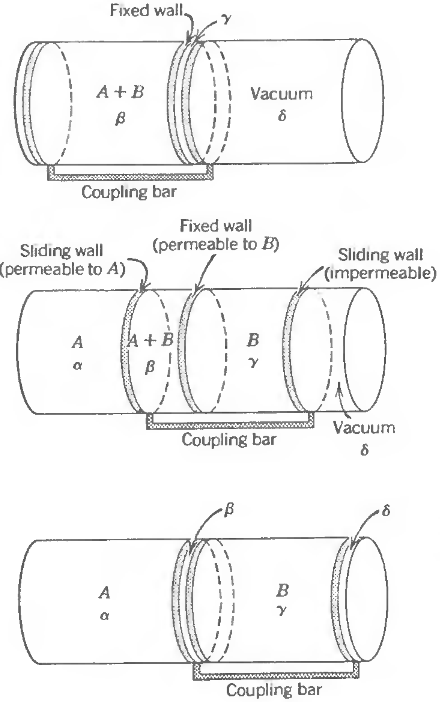
\includegraphics[width=.5\textwidth]{Pictures/fig3.2.png}
\figcaption{分离混合理想气体,用以展示 Gibbs 定理。}
\label{fig3.2}
\end{figure}

左边的滑动隔板可以任由气体A通过,但无法通过气体B,中间的固定隔板可任由气体B通过,但无法通过气体A,右边的滑动隔板两种气体都无法通过.

然后,这两块链在一起的滑动隔板被向右准静态地推动,直至$V_\beta=V_\delta=0$且$V_\alpha=V_\gamma=V_0$. 此时小室$\alpha$中为纯的气体A,小室$\gamma$中为纯气体B. 最开始体积为$V_0$的混合物被分成了两种纯气体,每种纯气体的体积都为$V_0$. 假如Gibbs定理成立,则系统终态的熵应该等于最开始的熵,接下来可以看到,上面的思想实验证实了这个论断.

需要指出,\eqref{equ3.39}中的第二个方程说明能量仅是温度$T$与mole数的函数,这就确保系统终态的能量等于始态的能量. 因此$-T\Delta S$等于移动两个链在一起的滑动隔板所做的功.

气体A可以自由通过左边的隔板,因此在准静态过程中,小室$\alpha$中的A气体与小室$\beta$中的A气体达到平衡,二平衡条件是$\mu_{A,\alpha}=\mu_{A,\beta}$. 小室$\beta$和小室$\gamma$中的B气体也有类似的关系.习题3.4-14会证明由$\mu_{A,\alpha}=\mu_{A,\beta}$和$\mu_{B,\beta}=\mu_{B,\gamma}$可以推出
\begin{equation*}
P_\alpha=P_\gamma \qquad P_\beta=2P_\alpha
\end{equation*}
这就是说,作用在相链结的两块滑动板上的总压力$P_\alpha-P_\beta+\Phi_\gamma$(当然应该乘上作用面积S,不过在这里,两边的S都相等)为0. 因此移动滑板不需要做功,所以该过程中就没有熵变. 最开始体积为$V_0$的A、B混合物之熵,与纯体积都为$V_0$的纯气体A、B的熵是相等的. 这就是Gibbs定理.

最后,需要指出,本节中所考虑的简单理想气体是一般气体的一种特殊情况,现实中,很多气体在压强很小或适中的情况下都可以视作简单理想气体. 与简单理想气体相同,一般理想气体的(力学)状态方程也是$PV=NRT$,其内能也是温度的函数,但不再是线性的了. 一般的理想气体会在第13章中讨论,而利用统计力学推导基本方程的方法会现身于第16章.

\subsection*{习题}

\section{理想van der Waals流体}
\label{sec3.5}
三次元世界的气体不太符合理想气体方程,除非在密度极低的情况下。1873年,J. D. van der Waals提出了对理想气体力学状态方程\eqref{equ3.28}式的改进:
\begin{equation}
    P = \frac{RT}{v - b} - \frac{a}{v^2}.
\label{equ3.41}
\end{equation}
其中$a, b$是与特定气体有关的经验常数。它的定量结果有一定的改进,但在要求更高的应用领域,状态方程还得加上更多的修正项与经验常数(五个甚至更多)。不过van der Waals方程在描述三次元流体的定性特征方面取得了极大的成就,例如描述气-液相变。

van der Waals 修正项的动机具有启发意义,看上去比较可信,尽管这些动机超出了热力学的范围\mpar{后面会看到,这些动机涉及到了微观情形}。方程$P = RT/v$是假设理想气体压强由许多无相互作用的的分子质点不断撞击容器壁形成的,van der Waals对这一假设做了两个看上去合理的简单修正。第一个修正考虑到分子并非点粒子,它们每个都占据$b/N_A$的体积。从而理想气体方程的$V$替换为$V - Nb$;减小的体积$Nb$是分子自身占据的体积。

第二个修正来自分子之间的相互作用力。容器中部的分子受到附近各个方向的分子间作用力,从而相互抵消了。但是容器壁附近的分子受到内部分子净的向内的吸引力,从而减小了分子撞击器壁的等效压强。压强的减小量应该与相互作用的{\it 分子对}的数量成正比,亦即与单位体积分子数的平方($1/v^2$)成正比;这就是van der Waals方程的第二处修正。

统计力学会用更加定量、正规的方式导出van der Waals方程,而且还会揭示\eqref{equ3.41}之上的一系列更高阶修正项。截断高阶项得到的van der Waals方程良好描述了真实气体的{\it 定性}特征,在定量方面也有一定修正(但并未到最好)。

要完整定义一个热力学系统,除了van der Waals方程之外还需要一个热状态方程,它当然可以从实验出发钦点一个。但更有意义的做法是,尝试从van der Waals方程出发构造最简单、最合理的热方程。可惜不能简单套用现成的理想气体热状态方程,热力学对两个状态方程的限制使得这样不被允许,必须得改动一下理想气体版本。

将van der Waals方程写为
\begin{equation}
	\frac{P}{T} = \frac{R}{v - b} - \frac{a}{v^2} \frac{1}{T}.
\label{equ3.42}
\end{equation}
要构造的另一个状态方程的一般形式为
\begin{equation}
	\frac{1}{T} = f(u, v).
\label{equ3.43}
\end{equation}
从上两式就能导出单位摩尔数基本方程的微分形式
\begin{equation}
	\,\mathrm ds = \frac{1}{T}\,\mathrm du + \frac{P}{T}\,\mathrm dv.
\label{equ3.44}
\end{equation}
然后积分出基本方程。$\mathrm ds$是全微分要求$s$关于$u, v$的二阶混合导数必须相等:
\begin{equation}
	\frac{\partial^2 s}{\partial v \partial u} = \frac{\partial^2 s}{\partial u \partial v}.
\label{equ3.45}
\end{equation}
即
\begin{equation}
    \frac{\partial}{\partial v} \left( \frac{1}{T} \right)_u = \frac{\partial}{\partial u} \left( \frac{P}{T} \right)_v,
\label{equ3.46}
\end{equation}
带入具体形式得
\begin{align}
    \frac{\partial}{\partial v} \left( \frac{1}{T} \right)_u &= \frac{\partial}{\partial u} \left( \frac{R}{v - b} - \frac{a}{v^2} \frac{1}{T} \right)_v \notag \\
    &= -\frac{a}{v^2} \frac{\partial}{\partial u} \left( \frac{1}{T} \right)_v.
\label{equ3.47}
\end{align}
上式可写为
\begin{equation}
    \frac{\partial}{\partial (1/v)} \left( \frac{1}{T} \right)_u = \frac{\partial}{\partial(u/a)} \left( \frac{1}{T} \right)_v.
\label{equ3.48}
\end{equation}
这意味着$1/T$必须是$1/v$与$u/a$的函数,并且关于这两者的偏导数相等。一种可能的形式为$1/T$是它们的和的函数,即$1/T = 1/T(1/v + u/a)$. 考虑到简单理想气体满足$1/T = cR/u$; 这暗示修改得到的van der Waals方程最简单的 形式为
\begin{equation}
    \frac{1}{T} = \frac{cR}{u + a/v}.
\label{equ3.49}
\end{equation}
便利起见,今后把van der Waals状态方程\eqref{equ3.41}与\eqref{equ3.49}式所表征的(理想化的)热力学系统称为“理想van der Waals流体”。

应当注意,尽管\eqref{equ3.41}式通常被称为“van der Waals状态方程”,但它并非状态方程的标准形式。不过将\eqref{equ3.49}, \eqref{equ3.42}式联立可得
\begin{equation}
    \frac{P}{T} = \frac{R}{v - b} - \frac{acR}{uv^2 + av}.
\label{equ3.50}
\end{equation}
以上两式才是标准的熵表象状态方程,也就是将$1/T$和$P/T$表示为$u, v$的函数。

从这两个方程能够得到如下的热力学基本关系(读者自行推导):
\begin{equation}
    S = NR \ln \big[ (v - b)(u + a/v)^c \big] + Ns_0.
\label{equ3.51}
\end{equation}
其中$s_0$为积分常数。上式不满足Nernst定理(和理想气体基本方程一样),因此在低温下失效。

之后的第9章会讲到van der Waals流体在某些温度、压强下不稳定,这自然分隔成了两个相(“液相”与“气相”)。基本方程\eqref{equ3.51}式是阐释热力学原理的极好例子。

\begin{table}[h]
\centering
\begin{tabular}{c c c c}
    \toprule
    气体 & $a (\si{Pa \cdot m^6})$ & $b (10^{-6}\si{m^3})$ & $c$ \\
    \midrule
    \ce{He}	&	0.00346	&	23.7	&	1.5 \\
    \ce{Ne}	&   0.0215	&	17.1	&	1.5 \\
	\ce{H2}	&	0.0248	&	26.6	&	2.5 \\
	\ce{A}	&	0.132	&	30.2	&	1.5 \\
	\ce{N2}	&	0.136	&	38.5	&	2.5 \\
	\ce{O2}	&	0.138	&	32.6	&	2.5 \\
	\ce{CO}	&	0.151	&	39.9	&	2.5 \\
	\ce{CO2}&	0.401	&	42.7	&	3.5 \\
	\ce{N2O}&	0.384	&	44.2	&	3.5 \\
	\ce{H2O}&	0.544	&	30.5	&	3.1 \\
	\ce{Cl2}&	0.659	&	56.3	&	2.8 \\
	\ce{SO2}&	0.680	&	56.4	&	3.5 \\
    \bottomrule
\end{tabular}
\caption{常见气体的van der Waals常量与摩尔热容(引自Paul S Epstem.{\it Textbook of Thermodynamics, }Wiley, New York, 1937.)}
\label{tab3.1}
\end{table}

表\ref{tab3.1}给出了一些真实气体的van der Waals常量。$a, b$是通过拟合van der Waals流体在\SI{273}{\kelvin}附近的等温线得到的,温度偏离越远,等温线的拟合效果越不好。常量$c$是从室温摩尔热容得到的。

\subsection*{习题}

\section{黑体辐射系统}
\label{sec3.6}
对于器壁温度为$T$的“空”容器,其可以看做一个电磁能量的贮藏室。在量子理论家眼中,它是光子箱;在工程师心里,它是多种电磁模式并存的谐振腔;在经典热力学学者看来,它与上述任何力学模型都得划清界限。无论采用什么观点,这种电磁腔总是遵循来自实验的、经验性的状态方程——“Stefan-Boltzmann 定律”:
\begin{align}
    U &= bVT^4, \label{equ3.52} \\
    P &= \frac{U}{3V}. \label{equ3.53}
\end{align}
其中$b = 7.56 \times 10^{-16} \si{J / m^3 K^4}$,其值可以从16.8节的基本理论出发计算。注意,上面经验性的状态方程与$N$无关,只是$U$与$V$的函数。这提醒我们在“空的”容器中不存在用粒子数$N$计数的、数量守恒的粒子。电磁辐射腔的基本方程$S = S(U, V)$只含有两个(而非三个)独立的广延量!

从电磁辐射的两个已知的状态方程出发可以完整导出全部信息,只需把它们带入Euler关系:
\begin{equation}
    S = \frac{1}{T} U + \frac{P}{T} V
    \label{equ3.54}
\end{equation}
即可得到基本方程。

为此,将\eqref{equ3.52}与\eqref{equ3.53}式改写为
\begin{align}
    \frac{1}{T} &= b^{1/4} \left( \frac{V}{U} \right)^{1/4}, \label{equ3.55} \\
    \frac{P}{T} &= \frac{1}{3} b^{1/4} \left( \frac{U}{V} \right)^{3/4}. \label{equ3.56}
\end{align}
带入\eqref{equ3.54}式即得到基本方程
\begin{equation}
    S = \frac{4}{3} b^{1/4} U^{3/4} V^{1/4}.
\label{equ3.57}
\end{equation}

\subsection*{习题}


\section{橡胶带系统}
\label{sec3.7}
本节要建立橡胶带系统的物理模型,这是热力学的应用中画风有所不同的一种。我们会看到热力学是如何限制与引导建立简单系统的唯象模型的。

下面开始建立一个描述橡胶带特征的物理模型。橡胶带是一束聚合物分子长链,它的宏观特征量有长度$L$,张力$\mathscr{T}$,温度$T$以及内能$U$. 橡胶带系统与之前的简单系统广延量的类比关系大致为长度$L \sim $体积$V$,张力$\mathscr{T} \sim$ 负压强$-P$. 至于系统的粒子数$N$,也许可以比作橡胶带单体聚合物的数量(不过它通常是不变的,可以作为一个常数压缩进公式里消失掉)。

实验观测的定性结论可以总结为如下两点。首先,在长度一定的条件下,橡胶带的张力大小随温度的升高而{\it 升高}——这个性质与绷紧的金属条完全相反,真是太让人意外了。第二,实验表明橡胶带的能量其实与长度无关,至少在“弹性极限”(该极限对应于分子链不打结,或完全拉伸)范围内是这样。

第二个结论用最简单的公式表示为
\begin{equation}
    U = cL_0 T,
\label{equ3.58}
\end{equation}
其中$c$是常数,$L_0$(也是常数)是橡胶带未伸长时的自然长度。张力与长度的在自然长度$L_0$到弹性极限$L_1$范围内的线性关系表示为
\begin{equation}
    \mathscr{T} = bT \frac{L - L_0}{L_1 - L_0}, \quad L_0 < L < L_1.
\label{equ3.59}
\end{equation}
其中$b$是常数。上式右端出现的之所以是$T$(而不是$T^2$或$T$的其它函数),是热力学理论对两个状态方程限制的结果,就像\eqref{equ3.46}式那样,
\begin{equation}
    \frac{\partial}{\partial L} \left( \frac{1}{T} \right)_U = \frac{\partial}{\partial U} \left( -\frac{\mathscr{T}}{T} \right)_L,
\label{equ3.60}
\end{equation}
上式表明了$\eqref{equ3.59}$式右侧$T$的线性形式。从而
\begin{equation}
    dS = \frac{1}{T} dU - \frac{\mathscr{T}}{T} dL = cL_0 \frac{dU}{U} - b \frac{L - L_0}{L_1 - L_0} dL,
\label{equ3.61}
\end{equation}
解得基本方程为
\begin{equation}
    S = S_0 + cL_0 \ln \frac{U}{U_0} - \frac{b}{2(L_1 - L_0)} (L - L_0)^2.
\label{equ3.62}
\end{equation}

尽管这个基本方程是从定性的观测结果导出的,但它合理地描述了橡胶带的经验特性,更重要的是它与实验符合。这一模型体现了科学家利用热力学理论建立基本模型的过程。

第15章会用统计力学方法建立一个聚合物弹性体更复杂的模型。

\subsection*{习题}
\begin{enumerate}
    \item[3.7-1.] 利用橡胶带模型计算在张力一定、温度变化$\delta T$的条件下长度的相对变化$(L - L_0)$,结果用长度和温度表示。
    \item[3.7-2.] 温度$T$一定,橡胶带长度变化$dL$,计算相应的传入橡胶带的热量$\delta Q$,并计算外界对橡胶带做的功。二者之间有什么关系?为什么?
    \item[3.7-3.] 若未张紧的橡胶带的能量与$T$的平方成正比,即\eqref{equ3.58}式变成$U = cL_0 T^2$,那么\eqref{equ3.59}式是否需要变化?导出新的基本方程。
\end{enumerate}

\section{不可控变量;磁系统}
\label{sec3.8}
先前几节讲述了几个特定的热力学系统,它们体现了热力学理论广泛的适用性,以及对简单系统进行建模时给出的约束条件。本节讨论简单的磁系统。之前的例子已经反映了热力学的一般结构,而具体系统的“特质”与特定的热力学量有关,磁系统容易体现这种特异性(这也是本节讲述它的额外目的)。

简明起见,只考虑位于均匀外磁场中的椭圆型磁介质样品(保证磁场的均匀性),样品的主轴与外磁场平行。还假设磁结晶的各向异性不存在,或者即使存在,磁化容易方向\mpar{easy axis ,无外场时物体可能出现自发磁化的方向。}也与外场平行。此外,样品是顺磁性或逆磁性介质,也就是说,外场消失后,介质也不再磁化。只在最后讲述相变的内容里考虑铁磁相(能自发磁化的系统状态)。

表征这种磁系统磁状态的广延量是系统的磁偶极矩$I$(证明见附录B)。基本方程的形式为$U = U(S, V, I, N)$。稍普遍一点的情形是样品的椭球主轴与外场{\it 不}共轴,这时单个参量$I$要替换为磁矩的三个直角坐标分量,基本方程为$U = U(S, V, I_x, I_y, I_z, N)$. 不过简单情形就能体现热力学结构,我们采用这种方便的做法。

磁矩$I$对应的强度量是{\it 外磁场}$B_e$,也就是样品不存在时的磁场:
\begin{equation}
    B_e = \left( \frac{\partial U}{\partial I} \right)_{S, V, N}.
\label{equ3.63}
\end{equation}
$B_e$的单位是tesla(T), $I$的单位是Joule/Tesla(J/T).

必须提醒读者注意这些广延量与强度量定义的细微之处(具体见附录B)。内能$U$定义为磁系统独有的能量,它不包括系统占据的“真空”所具有的磁能$\frac{1}{2} \mu_0^{-1} B_e^2 V$ (其中$\mu_0 = 4\pi \times 10^{-7} \si{T m / A}$, 真空磁导率)。系统所在的这部分空间区域的{\it 总能量}是$U + \frac{1}{2} \mu_0^{-1} B_e^2 V$. “真空项”是否包含在系统内能当中只是定义上的问题,两种选择都可以(我们定义$U$不包括真空项),但如果对这两种情况不加以辨别则会造成相当多的困惑。再次强调,系统内能$U$是磁系统所占据空间的能量的{\it 变化};它不包括在系统之前就存在于这片区域的能量$\frac{1}{2} \mu_0^{-1} B_e^2 V$.

磁系统的Euler关系为
\begin{equation}
    U = TS - PV + B_e I + \mu N.
\label{equ3.64}
\end{equation}
Gibbs-Duhem关系为
\begin{equation}
    SdT - VdP + IdB_e + Nd\mu = 0.
\label{equ3.65}
\end{equation}
磁系统的特性体现在移除限制之后子系统的平衡态条件(有关讨论见\ref{sec2.7}, \ref{sec2.8}节)上。人们发现无法控制磁矩;{\it 实验中的磁矩总是不可控制的!}作用于样品的磁场{\it 可以}控制(就像改变压强那样),因而可以通过调控磁场使样品磁矩达到某个想要的值,甚至还可以不断调整磁场以使得磁矩保持不变——就像通过反馈装置调整气压以使体积不变那样。但与通过刚性壁来保持体积不变不同,{\it 不存在但限制磁矩不变的“壁”。}

尽管磁矩不可控制,热力学理论仍可应用于磁系统,基本方程、状态方程、Gibbs-Duhem关系、Euler关系仍然成立。磁矩的不可控制性看成是“单纯的实验疑难”就好了,它对热力学理论无重大影响。

最后给出磁系统的基本方程的一种具体形式\sout{用来出题}——简单顺磁性模型的基本方程:
\begin{equation}
    U = NRT_0 \exp \left[ \frac{S}{NR} + \frac{I^2}{N^2 I_0^2} \right].
\label{equ3.66}
\end{equation}
其中$T_0, I_0$是正的常数。这个模型不能描述任何实际系统——它是复杂模型、实际问题基于的简单化、理想化的模型,只是为了描述热磁作用的特征性质。更多相关性质的讨论参见本节习题。

磁系统可以作为简单系统推广化的样例,故而在结束本节之后,我们将回到简单系统,深入讨论它的热力学性质。

\subsection*{习题}


\section{摩尔热容与其他导出量}
\label{sec3.9}
我们已经看到基本方程中的一阶微分具有重要的物理意义. 而不少二阶微分描述了物质性质,在物理上更易于引起关注,因此我们将考察一些特别的二阶微分量并阐述其作用. 之后,在第\ref{chap7}章中,我们将以一种更规整的结构回过头来学习这些二阶微分量,在那里你会看到只有很小一部分二阶微分是独立的,其他的都可以通过一种自成体系的“约化规则”与这些独立量相关联. 对于不考虑磁作用的简单系统,基本的微分量(诸多其他的微分量与这些基本的量相关)只有三组.

{\it 热膨胀系数(coefficient of thermal expansion)}\mpar{即定压膨胀系数}定义为
\begin{equation}
\label{equ3.67}
\alpha=\frac{1}{v}\left(\frac{\partial v}{\partial T}\right)_P=\frac{1}{V}\left(\frac{\partial V}{\partial T}\right)_P
\end{equation}
它描述了系统压强恒定(组分的摩尔数也恒定)的情况下,增加一个单位温度后,系统体积的相对增量.

{\it 等温压缩系数(isothermal compressibility)}定义为
\begin{equation}
\label{equ3.68}
\kappa_T\equiv-\frac{1}{v}\left(\frac{\partial v}{\partial P}\right)_T=\frac{1}{V}\left(\frac{\partial V}{\partial P}\right)_T
\end{equation}
它描述了系统温度恒定(组分的摩尔数也恒定)的情况下,增加一个单位压强后,系统体积的相对增量.

{\it 摩尔定压热容系数(molar heat capacity at constant pressure)}定义为
\begin{equation}
\label{equ3.69}
c_P=T\left(\frac{\partial s}{\partial T}\right)_P=\frac{T}{N}\left(\frac{\partial S}{\partial T}\right)_P=\frac{1}{N}\left(\frac{\dbar Q}{\text{d}T}\right)_P
\end{equation}
它描述了系统压强恒定(组分的摩尔数也恒定)的情况下,让体系的温度增加一个单位所需的热量.

对于组分的摩尔数恒定的系统,其他的二阶微分量都可以由这三个来表示,所以这三个量在不同压强和温度下的值常被人们制成表格.

二阶微分量之间的关系怎么导出?原则上,我们可以这样想(更完整的表述在第\ref{chap7}章中).最简单的关系也许是:
\begin{equation}
\label{equ3.70}
\left(\frac{\partial T}{\partial V}\right)_{S,N}=-\left(\frac{\partial P}{\partial S}\right)_{V,N}
\end{equation}
由微积分的基本知识可知,$U$对$S,V$的二阶混合偏导数相等
\begin{equation}
\label{3.71}
\frac{\partial}{\partial V}\left(\frac{\partial U}{\partial S}\right)=\frac{\partial}{\partial S}\left(\frac{\partial U}{\partial V}\right)
\end{equation}
由此即得\eqref{equ3.70}

\eqref{equ3.70}中的两个(二阶微分)量具有很直观的物理意义,而且都可被直接测量. $\left(\frac{\partial T}{\partial V}\right)_{S_N}$对应绝热过程中温度随体积的变化率;而$-\left(\frac{\partial P}{\partial S}\right)_{V,N}$可以写作$T\left(\frac{\text{d} P}{\dbar Q}\right)_{V,N}$则是压强与输入系统的热量$\text{d}Q$之比(在体积不变的情况下).这两个看起来毫无关系的量被联系在了一起,这是很不简单的结果,实际上,这是热力学理论的第一次“胜利”. 毫无疑问,实验结果也支持这个等式.

\eqref{equ3.70}在熵表象下的表达式为:
\begin{equation}
\label{equ3.72}
\frac{\partial }{\partial V}\left(\frac{1}{T}\right)_{U,N}=\frac{\partial }{\partial U}\left(\frac{P}{T}\right)_{V,N}
\end{equation}
我们马上就可以发现,这个就是我们在\eqref{equ3.46}中为了求van der Waals方程对应的热状态方程所引入的等式.

在第\ref{chap7}章中,我们将看到,这些等式实际上就是一类很普遍的类似关系(被称作Maxwell关系)\mpar{原文“analogous relationship”}的原型.Maxwell关系以简洁的形式将两个二阶微分量联系在一起,实际上,Maxwell关系是一个更加普适的定理的退化形式,该定理表明,任意{\it 四}个微分量之间必然有一个关系.这些关系让我们能将任意一个二阶微分量用“基本集”\mpar{所谓基本集,就是由$c_p,\alpha,\kappa_T$这些既基础且有明确物理意义的量组成的集合——译者注.}中的元素$c_p,\alpha,\kappa_T$表示出来(在恒定$N$的情况下).

为了阐明这些预想的关系,我们先额外引入两个具有实际意义的二阶微分量;绝热压缩率$\kappa_S$\mpar{关于此处$S$的大小写,原文如此。}和定压摩尔热容$c_v$.

$\it{绝热压缩率 (isomethermal compressibility)}$定义如下:
\begin{equation}
\label{equ3.73}
\kappa_s=-\frac{1}{v}\left(\frac{\partial v}{\partial P}\right)_s=-\frac{1}{V}\left(\frac{\partial V}{\partial P}\right)_S
\end{equation}
它表征了熵恒定的情况下(比如绝热系统),体积在压强变化时的下降率.

$\it{定压摩尔热容 (molar heat capacity at constant pressure)}$定义如下:
\begin{equation}
\label{equ3.74}
c_v=T\left(\frac{\partial s}{\partial T}\right)_v=\frac{T}{N}\left(\frac{\partial S}{\partial T}\right)_V=\frac{1}{N}\left(\frac{\dbar Q}{\text{d}T}\right)_V
\end{equation}
它表征了恒容准静态过程中,体系中一摩尔物质的温度每升高一度所需要的热量(也就是热量除以体系的物质的量).

在第\ref{chap7}章中,我们会证明
\begin{equation}
\label{equ3.75}
c_P=c_v+\frac{TV\alpha^2}{N\kappa_T}
\end{equation}
以及
\begin{equation}
\label{equ3.76}
\kappa_T=\kappa_S+\frac{TV\alpha^2}{Nc_P}
\end{equation}
再次强调,这里我们并不需要将注意力放在\eqref{equ3.75}\eqref{equ3.76}这两个式子的的细节上,而是要引起读者对三个基本量$c_p;\alpha;\kappa_T$的注意,通过这三个基本量,我们可以将所有其他的微分量表示出来(比如$c_v;\kappa_S$),因此这三个基本量关于$T,P$的函数常被列作表格以资查阅利用.如何更加系统地导出这些等式?如何方便的记忆它们?我们将在第\ref{chap7}章详细介绍.

推荐学生做做习题3.9-6.
\begin{example}
一种物质的$c_p,\alpha,\kappa_T$关于$T,P$的函数已被做成表格(即已知它们关于$T,P$的函数).试找出摩尔体积$v$关于$T,P$的函数
\texttt{解答}
我们在$T-P$平面上考虑问题. $c_p,\alpha ,\kappa_T$关于$T,P$的函数值在全平面上都已知,然后我们试图寻找$v(T,P)$的表达式,首先
\begin{align}
\text{d}v&=\left(\frac{\partial v}{\partial P}\right)_T\ \text{d}P+\left(\frac{\partial v}{\partial T}\right)_P\ \text{d}T\\
&=-v\kappa_T\ \text{d}P+v\alpha\ \text{d}T
\end{align}
    或
\[\frac{\text{d}v}{v}=-\kappa_T\ \text{d}P+\alpha\ \text{d}T\]
如果选$(T_0,P_0)$为参考点,且$(T^\prime,P^\prime)$是我们感兴趣的点,那么我们按照图示的路径进行积分(或者你可以选择任意一条合适的路径).对于我们选定的这个路径而言,在它的水平段上,$\text{d}T=0$,在它的竖直段上,$\text{d}P=0$,因此
\[\int\frac{dv}{v}=\int_{T_0}^{T^\prime}\alpha(T,P_0)\ \text{d}T-\int_{P_0}^{P^\prime}\kappa_T(T^\prime,P)\ \text{d}P\]
    或写成
\[\ln{\frac{v^\prime}{v_0}}=\int_{T_0}^{T^\prime}\alpha(T,P_0)\ \text{d}T-\int_{P_0}^{P^\prime}\kappa_T(T^\prime,P)\ \text{d}P\]
需注意,我们需要确定$v_0$时的摩尔体积,因为接下来我们将把其他时候的体积与$v_0$时的摩尔体积关联起来.

{
    \centering
    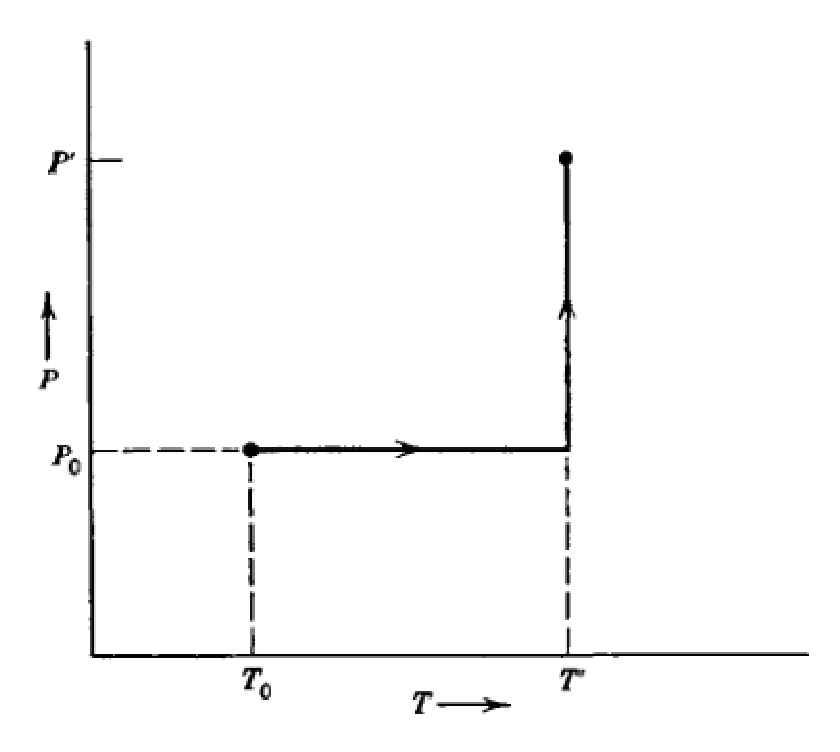
\includegraphics[scale=0.7]{fig3_9.eps}
}
\end{example}

\subsection*{习题}

%!TEX root = ../CallenThermo.tex

\chapter{可逆过程和最大功定理}\label{chap4}

\section{可能和不可能的过程}\label{sec4.1}

一名工程师常会需要通过设计一个装置来完成某个任务——例如让一个电梯升到高楼上。因此他就得弄出一个联动装置,或者“引擎”,来可控的将能量从火炉里转移到电梯上;{\it 如果}火炉里的热量通过数个活塞、杠杆和凸轮转换成了电梯上升所需要的能量。但谋事在人,成事由“天”(例如,物理定律)%
\mpar{原文为 "But 'nature'(i.e. the law of physics) exercise the crucial decision"}%
——这件事到底是能办成呢,还是设备干脆就停着不动,没有热量从火炉里出来,电梯也没上升一丝一毫。结果得取决于两点。其一是引擎得要满足力学定律(自然包括能量守恒),其二,这个过程必须最大化地使熵增加。\mpar{此处存疑,热力学过程只需满足熵增即可,略微偏离平衡区的线性系统才存在有最大熵产生定理。}

专利局里充满了各路在逻辑上无可挑剔的(如果A发生那么B一定发生)失败发明——这些天才般的设计满足所有力学定律,但依旧固执的停在那儿,默默地拒绝熵的减小。其他的一些能动起来,但会产生一些意料之外的结果,比发明者预料中更有效的使熵增加。

如果,虽然如此,这个网络被在保证总能量不变的前提下最大可行的增加总的熵,那么将不会有什么基本定律来否决掉这样一个恰当的过程的存在。尽管实现这样适当的引擎可能需要相当的天才成分,但它起码在原则上来讲是可行的。

\begin{example}\label{eg4.1}
一个约束系统具有确定摩尔数和体积,则其不能对外界做功。另外,这个系统的热容是常数$C$。则这个系统的基本方程是$S=S_0+C\ln(U/U_0)$,其中$U=CT$。\\
两个具有相同热容量的此类系统,初态分别具有温度$T_{10}$和$T_{20}$,其中$T_{10}<T_{20}$。一个用于升降电梯的引擎(即对一个纯力学系统做功),从这两个热力学系统中获取能量。它们最大能获得多少功?\\
{\bf 求解:}\\
这两个热力学系统最终会达到相同的温度$T_f$。其能量的总改变量为
\[
\Delta U = 2CT_f-C(T_{10}+T_{20})
\]
而力学系统(“电梯”)所获得的功为$W=-\Delta U$,即
\[
W = C(T_{10}+T_{20}-2T_f)
\]
熵的总改变量为两个热力学系统的改变量之和,为
\[
\Delta S = C\ln\frac{T_f}{T_{10}} + C\ln\frac{T_f}{T_{20}} = 2C\ln\frac{T_f}{\sqrt{T_{10}T_{20}}}
\]
为了使$W$最大,我们自然希望$T_f$最小(从第二式容易看出),根据第三式我们知道这意味着要使$\Delta S$取极小。而$\Delta S$最小就只能是零了,对应着一个可逆过程。这样最优的引擎能得到
\[
T_f = \sqrt{T_{10}T_{20}}
\]
和
\[
W = C(T_{10}+T_{20}-2\sqrt{T_{10}T_{20}})
\]
\end{example}

作为补充,我们需要注意到假设两个热力学系统最后到达一个相同的温度是不必要的;$W$可以分别对$T_{1f}$和$T_{2f}$作优化,最后能得到同样的结果。对于末温相同这个简化假设,我们可以用自洽性来论证:如果末温不同,那么我们可以通过这个办法来继续获取更多的能量。

\begin{example}
例\ref{eg4.1}的一个有趣的变体是三物体(每一个都是例\ref{eg4.1}中描述的类型,有$U=CT$)初始温度分别为\SI{300}{\kelvin}、\SI{350}{\kelvin}、\SI{400}{\kelvin}。其需求是尽可能高的提高{\it 一个}物体的温度,而不论其他两个物体怎么样(并且不改变任何外部系统的状态)。那么这里一个物体最高能到多高温度?\\
{\bf 求解:}\\
将三个初始温度用$T_1$,$T_2$,$T_3$标记,单位取作\SI{100}{\kelvin}($T_1=3$,$T_2=3.5$以及$T_3=4$)。类似的,令单个物体能达到的最高温度记做$T_h$。可以推断剩下两个物体的末温{\it 都}是$T_c$(否则,我们可以用例\ref{eg4.1}的办法来对外做功,然后将功转换为热物体上的热)。能量守恒要求
\[
T_h + 2T_c = T_1 + T_2 + T_3 = 10.5
\]
总的熵增为
\[
\Delta S = C\ln\frac{T_c^2T_h}{T_1T_2T_3}
\]
熵增为正要求
\[
T_c^2T_h \ge T_1T_2T_3 \quad (=42)
\]
利用能量守恒式消去$T_c$
\[
(5.25-\frac{T_h}{2})^2T_h\ge 42
\]
方程左端对$T_h$作图。绘图范围从$0$到$10.5$,上界是为了保证$T_c$为正。图像表明使纵坐标大于$42$的最大$T_h$值是
\[
T_h = 4.095 \quad(\text{或}T_h = \SI{409.5}{\kelvin})
\]
这个值使不等式取等,即对应可逆过程。
\end{example}
\begin{figure}
\centering
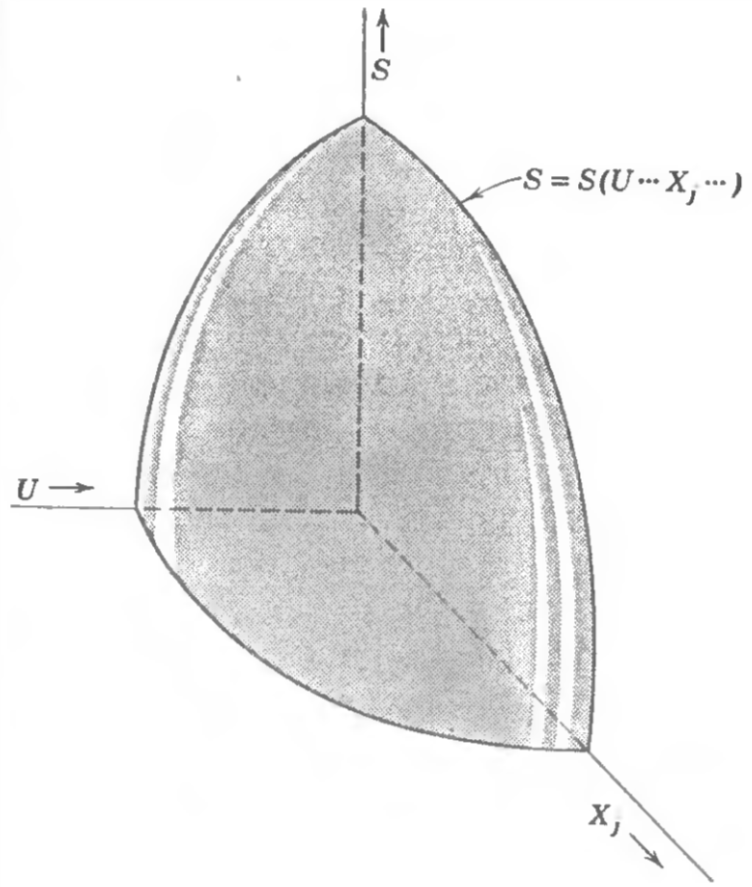
\includegraphics[width=\textwidth]{Pictures/fig4.1.png}
\end{figure}

这道题的另一个解法见习题4.6-7。

\subsection*{习题}
\begin{itemize}
\item[4.1-1.] 一摩尔单原子理想气体和一摩尔$c=3/2$的理想 van der Waals 流体(\ref{sec3.5}节)分别装在体积为$v_1$和$v_2$的容器里。理想气体的温度为$T_1$而 van der Waals 流体是$T_2$。我们希望将理想气体的温度变成$T_2$而保持总的能量不变。那么 van der Waals 流体的末温是多少?各参数($T_1,T_2,a,b,v_1,v_2$)之间需要满足什么关系才能实现这样一个温度转换(总是假定在过程中外界不发生改变)?
\item[4.1-2.] 一个橡胶带(\ref{sec3.7}节)初始温度为$T_B$,长度为$L_{B}$。一摩尔单原子理想气体初温为$T_G$,体积为$V_G$。理想气体经历一个定容升温过程达到温度$T_G'$。其所需要的能量全都从橡胶带中获得。那么橡胶带的长度是否需要改变?如果是的话,改变多少?
\begin{flushright}
{\it 答案:}\\
若$l=L_B-L_0$,
\[
l^2-(l')^2\ge 2b^{-1}cL_0(L_1-L_0)\ln\left(1-\frac{3R}{2RL_0}\frac{T_G'-T_G}{T_B}\right)+3Rb^{-1}(L_1-L_0)\ln(T_G'/T_G)
\]
\end{flushright}
\item[4.1-3.] 假设例\ref{eg4.1}中的两个系统热容具有形式$C(T)=DT^n$,其中$n>0$:\\
\begin{enumerate}
\item 证明这样的系统内能$U=U_0+DT^{n+1}/(n+1)$以及熵$S=S_0+DT^n/n$。系统的基本方程是什么?
\item 如果其初始温度分别为$T_{10}$和$T_{20}$,最大可输出功为多少(两系统最后处于相同温度)?
\end{enumerate}
\begin{flushright}
{\it 答案:}\\
对于$n=2$:
\[
W=\frac{D}{3}\left[T_{10}^3+T_{20}^3-\frac{1}{\sqrt{2}}(T_{10}^2+T_{20}^2)^{3/2}\right]
\]
\end{flushright}
\end{itemize}
%!TEX root = ../CallenThermo.tex
%翻译:碘化亚铜
%校对:lh, Surgam Identidem
\chapter{其它表象,Legendre变换}
\label{chap5}

\section{能量最小原理}
\label{sec5.1}

之前的章节已经得到了熵最大原理最显著最直接的一些推论,进一步的推论会导出其它很多有用的基本结论。不过本章要重新审视理论的形式框架,并且注意到用一些等价的数学形式可以重新构造出相同的内容,这对深化发展热力学理论十分有益。这些其它的形式(表象)会在一些特殊类型的问题中显得特别方便,而热力学计算的艺术经常体现在选取对于给定的问题最适用的某种形式(表象)上。在恰当的表象下热力学问题会变得极为简单,而在不恰当的表象下会变得极为复杂。

力学中也会出现多种等价的形式——Newton形式,Lagrange形式,Hamilton形式。同样也会有某一问题用Lagrange形式处理会比用Newton形式更加容易处理的请况,反之亦然。但是不同形式(表象)导致的难易不同在热力学中表现得极为显著。正因如此,{\it 等价表象之间的一般变换理论是热统计理论的基础之一}。

之前实际上已经考虑过了两种等价的表象——能量表象和熵表象。但基本的极值原理却只在熵表述中构造出来。如果这两种表述的理论地位相同,我们就必须找出能量表象中与熵最大原理类似的极值原理,它确实存在。熵最大原理等价于能量最小原理,二者可相互替代。熵最大原理表明,在总能量的给定的条件下,平衡态对应于熵取最大值的状态。能量最小原理则表明对于给定总熵的平衡态,能量取最小值。

{
  \centering
  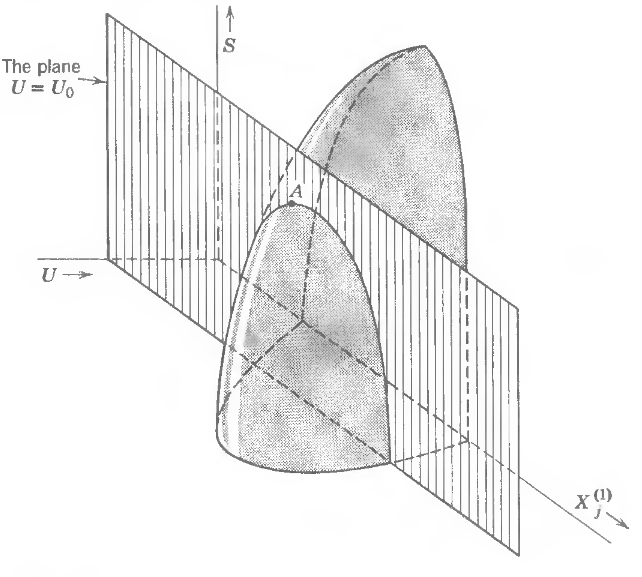
\includegraphics[width=0.6\textwidth]{fig5.1.png}
  \figcaption{平衡态$A$在给定$U$时$S$取极大。}
  \label{fig5.1}
}

图\ref{fig5.1}展示了\ref{sec4.1}节讨论的复合系统位形空间的剖面图。标记为$U$和$S$的轴对应复合系统的总能量和总熵,而标记为$X_j^{(1)}$的轴则对应着第一个子系统的某个广延量。其它没有在图中显示的轴还包括$U^{(1)}$,$X_j$以及其它的$X_k^{(1)}$和$X_k$。

复合系统的总能量是一个由封闭条件决定的常数。这个封闭条件的几何表示是系统的态处于图\ref{fig5.1}中$U=U_0$的平面上。系统的基本方程表示为图中的曲面,因此表示系统状态的点一定位于曲面和平面相交得到的曲线上。如果参数$X_j^{(1)}$不受约束,那么平衡态就是曲线上使得熵最大的态,也就是图\ref{fig5.1}中标记为A的态。

{
	\centering
	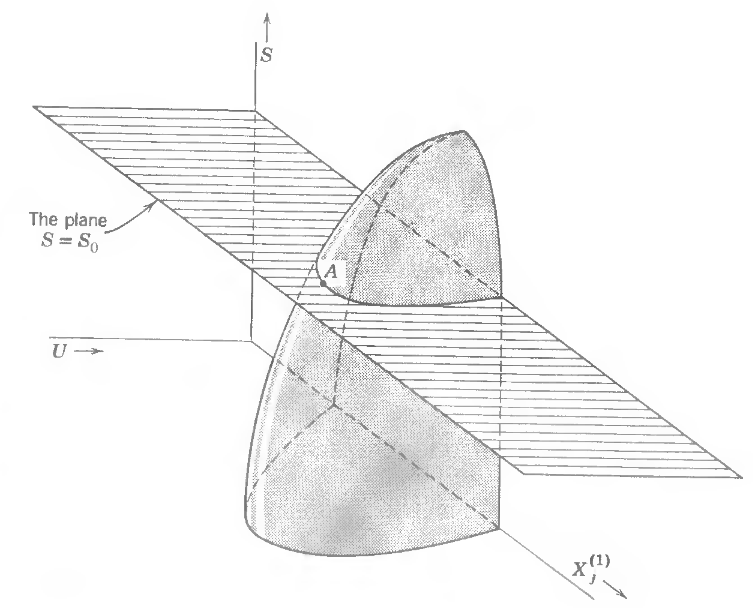
\includegraphics[width=0.6\textwidth]{fig5.2.png}
	\figcaption{平衡态$A$在给定$S$时$U$取极小。}
	\label{fig5.2}
}

在另一种表象下,平衡态A可以视为给定熵的能量最小态 —— 如图\ref{fig5.2}所示。经过平衡态点A的平面$S=S_0$与基本曲面\mpar{基本方程所对应的曲面}相交定义了一条曲线。这条曲线包含了一族熵为常数的态,{\it 而平衡态A则是曲线上能量最小的态}。

如图\ref{fig5.1}和\ref{fig5.2}所示,熵最大和能量最小原理的等价性明确依赖于基本曲面的几何形状,这个性质是普遍的。\ref{sec4.1}节讨论过,基本曲面的形状是由$\partial S/\partial U>0$以及$U$是关于$S$的单值连续函数这两个假设决定的;因此这两个关于解析性质的假设是两个原理等价的隐含条件。

总结一下,尽管尚未证明,但以下两个原理看起来是等价的:

{\bf 熵最大原理.}{\it 在总的内部能量确定时,任何不受约束的内部参量在平衡时的取值都使得熵最大}。

{\bf 能量最小原理.}{\it 在总的熵确定时,任何不受约束的内部参量在平衡时的取值都使得能量最小}。

两个极值准则等价性的证明既可以用物理论证,也可以用数学的方式阐述。首先考虑物理论证,下面说明如果能量{\it 不是}最小值的话,熵就可以不是最大值,并且反之亦然。

假设系统处于平衡态但能量并{\it 不是}在给定的熵下可能的最小值。这样就可以在保持熵为常数的同时从系统中提取能量(通过做功),并且随后就可以通过传热把这部分能量返还给系统。这样系统的熵会增加($\dbar Q=T\, \rd S$),于是系统恢复到它初始的能量,但是熵增加了。这跟初始的平衡态是熵最大的态是矛盾的!因此我们不得不推断最初的平衡态必须具有给定的熵下最小的能量。

相反的推论,也就是最小能量要求最大的熵,可以用类似的方式构造(见习题5.1-1).

下面是更形式化的证明,先假设熵最大原理成立:
\begin{equation}
\label{equ5.1}
\left(\frac{\partial S}{\partial X}\right)_U=0
~\text{及}~
\left(\frac{\partial^2 S}{\partial X^2}\right)_U<0
\end{equation}
在此为了简便,我们将$X_j^{(1)}$写作$X_j$,这暗示着其它的$X$将保持为常数。同时为了简便,我们暂时将一阶导数$(\partial U/\partial X)_S$记为$P$。于是根据(根据附录A中的公式A.22)可得:
\begin{equation}
\label{equ5.2}
	P \equiv \left( \frac{\partial U}{\partial X} \right)_S = -\frac{ \left( \dfrac{\partial S}{\partial X} \right)_U }{ \left( \dfrac{\partial S}{\partial U}\right)_X } = -T \left(\frac{\partial S}{\partial X}\right)_U = 0
\end{equation}
由此可推断$U$是极值。为了分清这个极值是极大极小还是拐点,我们必须研究二阶导数$(\partial^2U/\partial X^2)_S\equiv(\partial P/\partial X)_S$的正负。但是如果将$P$当做$U$和$X$的函数,则有:
\begin{align}
	\left(\frac{\partial^2 U}{\partial X^2}\right)_S &=\left(\frac{\partial P}{\partial X}\right)_S =\left(\frac{\partial P}{\partial U}\right)_X \left(\frac{\partial U}{\partial X}\right)_S +\left(\frac{\partial P}{\partial X}\right)_U =\left(\frac{\partial P}{\partial U}\right)_XP +\left(\frac{\partial P}{\partial X}\right)_U \label{equ5.3} \\
	&= \left( \frac{\partial P}{\partial X} \right)_U. \quad (P=0) \label{equ5.4} \\
	&= \frac{\partial}{\partial X} \left[- \frac{ \left( \dfrac{\partial S}{\partial X} \right)_U }{ \left( \dfrac{\partial S}{\partial U}\right)_X } \right]_U \label{equ5.5} \\
	&= -\frac{\dfrac{\partial^2 S}{\partial X^2}} {\dfrac{\partial S}{\partial U}} + \frac{\partial S}{\partial X} \frac{\dfrac{\partial^2 S}{\partial X \partial U}}{\left(\dfrac{\partial S}{\partial U}\right)^2} \label{equ5.6} \\
	&= -T\frac{\partial^2 S}{\partial X^2}>0 \quad \left( \frac{\partial S}{\partial X}=0 \right) \label{equ5.7}
\end{align}
因此$U$是一个极小值。反向的论证在形式上是一样的。

以前说过,两个极值条件完全等价的事实类似于几何中的等周问题。也就是一个圆既可以描述为给定周长下面积最大的二维图形,也可以描述为给定面积下周长最小的二维图形。

这两个描述圆的极值条件是完全等价的,每一个都适用于所有的圆。只不过它们给出两种不同的生成圆的方法。如果要把正方形连续变形为一个圆,我们可以保持它的面积是常数并且允许它的边像橡皮筋一样收缩。这样我们得到了作为给定面积下周长最小图形的一个圆。等价地,我们也可以保持正方形的周长不变并允许面积增加,这样就得到了作为给定周长下面积最大图形的一个(不同的)圆。尽管如此,在得到这些圆之后,{\it 每一个圆都同时满足自身取值下面积和周长的极值条件}。

关于热力学系统的物理情形跟上面描述的几何情形是非常类似的。也就是说,任何一个平衡态既可以描述为给定能量下熵最大的态,也可以描述为给定熵下能量最小的态。但是这两个条件却给出了两个不同的达到平衡态的方法。

作为这两种达到平衡方法的一个特定的例子,考虑一个最初固定在封闭圆柱某个位置的活塞。如何在移除活塞位置的限制之后使系统达到平衡态?我们可以简单地移去约束来使它自发达到平衡;此时由于封闭条件,能量会保持为常数而熵会增加。这个过程就是熵最大原理所要求的过程。此外,我们可以让活塞非常缓慢地移动,可逆地对外做功直到它到达两边压强相等的位置。在这个过程中能量从系统中提取出来,但是系统的熵保持为常数(这个过程是可逆的且没有热流)。这个过程就是能量最小原理要求的过程。
我们想强调的关键事实是,{\it 这两个过程以及其它任意过程最终达到的平衡态都满足两大极值原理。}%
\mpar{当然,从一个初态出发,通过不同的过程会到达不同的平衡态。}%
。

为了进一步说明最小能量原理,下面用它来解决\ref{sec2.4}节的热平衡问题(那里是用最大熵原理解决的)。考虑内部由固定的透热壁分隔的封闭复合系统,热量可以在两个子系统间自由流动,下面来找出它的平衡态。

能量表象下的基本方程是
\begin{equation}
\label{equ5.8}
U=U^{(1)}(S^{(1)},V^{(1)},N^{(1)}_1,\ldots)+U^{(2)}(S^{(2)},V^{(2)},N^{(2)}_1,\ldots)
\end{equation}
所有的体积和摩尔数都是已知常数,需要计算$S^{(1)}$和$S^{(2)}$。
暂时忽略系统封闭导致的总能量不变的事实,{\it 如果}允许能量改变的话,平衡态对应于能量最小的态。两个子系统之间虚拟热流引起总能量的虚拟变化为:
\begin{equation}
\label{equ5.9}
\,\mathrm dU=T^{(1)}\,\mathrm dS^{(1)}+T^{(2)}\,\mathrm dS^{(2)}
\end{equation}
能量最小条件也就是$\rd U = 0$,在总熵不变的条件下:
\begin{equation}
\label{equ5.10}
S^{(1)}+S^{(2)}=\text{constant}
\end{equation}
会有
\begin{equation}
\label{equ5.11}
\mathrm dU=(T^{(1)}-T^{(2)})\,\mathrm dS^{(1)}=0
\end{equation}
于是可得
\begin{equation}
\label{equ5.12}
T^{(1)}=T^{(2)}
\end{equation}

从而能量最小原理给出了与前面用熵最大原理得到的相同的热平衡条件。

方程\eqref{equ5.12}是一个关于$S^{(1)}$和$S^{(2)}$的方程。在总能量$U$已知,因此仅有的两个未知量是$S^{(1)}$和$S^{(2)}$的情况下,第二个方程选为方程\eqref{equ5.8}最为方便。理论上方程\eqref{equ5.8}和\eqref{equ5.12}会给出这个问题的精确解。

用完全一样的思路,可以发现一个内部有可动绝热壁的封闭系统的平衡条件是压强相等。这个结论在能量表象中是非常直接的,但是如同在\ref{sec2.7}的最后一段看到的,在熵表象中相对更加微妙。

\subsection*{习题}

\section{Legendre变换}
\label{sec5.2}

在能量表象和熵表象中,广延量都作为数学上的独立变量,而强度量都视为被导出的物理量。这与现实中实验操作的便利性截然不同。实验者经常发现强度量更容易测量和控制,因此更喜欢把强度量当成操作上的独立变量而把广延量当成导出量。最突出的是熵和温度这一对共轭变量:并不存在可以测量和控制熵的实验仪器,而测量和控制温度的温度计和恒温器在实验室中十分常见。于是,能否改变数学形式使得强度量代替广延量成为数学上的独立变量?当然可以,而且这样还能够导出很多其它的热力学表象。

重要的事情说三遍:不论是在熵表象还是能量表象下热力学都是逻辑完备且独立的,而介绍这些表象变换只是为了方便。大家公认这是一种使热力学避免了繁琐推导的简化。但原则上讲这只是某种捷径,并不是逻辑上所必须的。

下面给出表象变换的严格表述。设系统的基本方程已知:
\begin{equation}
\label{equ5.13}
	Y=Y(X_0,X_1,\ldots,X_t)
\end{equation}
我们想找到一个将导数
\begin{equation}
\label{equ5.14}
	P_k\equiv\frac{\partial Y}{\partial X_k}
\end{equation}
作为独立变量,但是不改变基本关系\eqref{equ5.13}中任何其他信息的方法。在几何和其他一些物理领域中也有与之类似的问题。这个问题需要采用名为Legendre变换的数学手段,它的几何意义十分直观,下面先来介绍Legendre变换的几何意义。

{
	\centering
	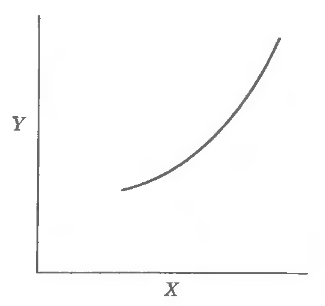
\includegraphics[width=.5\textwidth]{fig5.3.png}
	\figcaption{}
	\label{fig5.3}
}

简便起见,首先考虑基本方程只与一个独立变量$X$有关的情形:
\begin{equation}
\label{equ5.15}
	Y=Y(X)
\end{equation}
几何上,这个基本关系可表为直角坐标$X, Y$空间中的一条曲线(图\ref{fig5.3}),而导数
\begin{equation}
\label{equ5.16}
	P\equiv\frac{\partial Y}{\partial X}
\end{equation}
是这个曲线的切线斜率。如果想用$P$代替$X$作为独立变量,我们的第一反应可能是简单地用方程\eqref{equ5.15}和\eqref{equ5.16}消去$X$,从而得到$Y$关于$P$的函数
\begin{equation}
\label{equ5.17}
	Y=Y(P)
\end{equation}
从几何上容易看出,这样做无论如何都会在数学上牺牲掉基本关系\eqref{equ5.15}式的一些信息。显然对于$Y$关于斜率$\rd Y / \rd X$的函数的了解并不能让我们重构出曲线$Y=Y(X)$。实际上,图\ref{fig5.4}中每一条替代的曲线都等价地满足关系$Y=Y(P)$。

从分析的观点来看,关系$Y=Y(P)$是一个一阶微分方程,而它的积分给出的结果跟$Y=Y(X)$差一个待定的积分常数。由此可见,如果用$Y=Y(P)$代替$Y=Y(X)$成为基本方程,就会丢失掉基本关系中的一些原始信息。尽管我们希望让$P$成为一个数学上的独立变量,但这样做导致的信息丢失使得该方案完全不可行。

{
	\centering
	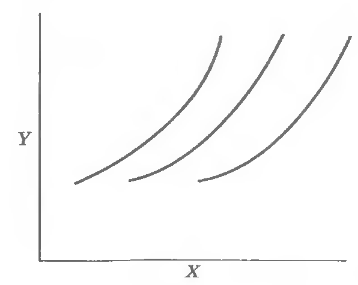
\includegraphics[width=0.6\textwidth]{Pictures/fig5.4.png}
	\figcaption{}
	\label{fig5.4}
}

靠谱的做法是由传统的{\it 点几何(point geometry)}与Pluecker的{\it 线几何(line geometry)}的对偶关系给出的。线几何的基本概念是一条给定的曲线可以很好地由以下两种方式等价描述:

\begin{itemize}
\item[(a)] 作为一族切线的包络线(图\ref{fig5.5});
\item[(b)] 作为满足关系$Y=Y(X)$的点的轨迹。
\end{itemize}

任何可以构造出一族切线的方程都能和关系$Y=Y(X)$一样好地决定一条曲线。

{
	\centering
	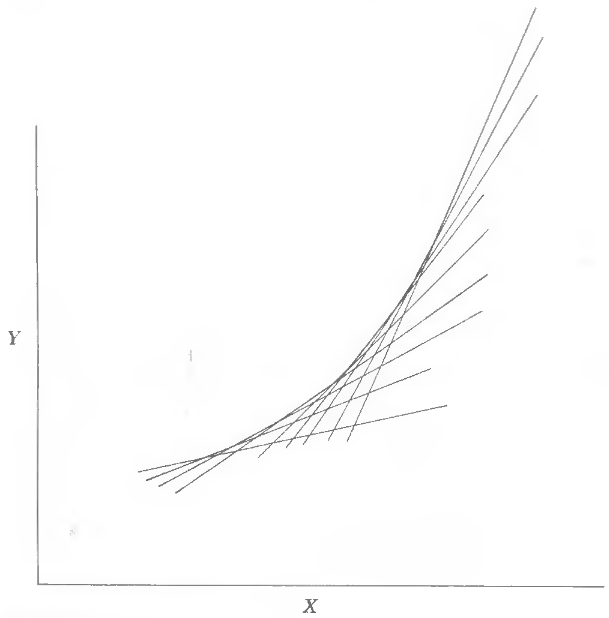
\includegraphics[width=0.5\textwidth]{Pictures/fig5.5.png}
	\figcaption{}
	\label{fig5.5}
}

正如平面上的每一个点都可以由两个数$X$和$Y$描述,平面上的每一条直线也都可以用两个数$P$和$\psi$描述,其中$P$是直线的斜率,$\psi$是它在$Y$轴上的截距。于是正如关系$Y=Y(X)$挑出了所有可能的点$(X,Y)$中的一个子集,关系$\psi=\psi(P)$挑出了所有可能的直线$(P,\psi)$的一个子集。关于切线的截距$\psi$作为斜率$P$的函数的知识可以让我们构造出一族切线,从而也就构造出了它们的包络线,也就是这条曲线。因此关系
\begin{equation}
\label{equ5.18}
	\psi=\psi(P)
\end{equation}
是跟基本关系$Y=Y(X)$完全等价的。在这个关系中,独立变量是$P$,于是方程\eqref{equ5.18}给出了对于自变量替换问题的一个圆满的解。由于关系$\psi=\psi(P)$跟关系$Y=Y(X)$是数学等价的,所以它也可以当成一个基本关系;$Y=Y(X)$是“$Y$表象”下的基本关系,而$\psi=\psi(P)$是“$\psi$表象”下的基本关系。

建议读者去画一些不同的斜率$P$和不同的$Y$轴截距$\psi=-P^2$的直线。可以看出关系$\psi=-P^2$描述了一条抛物线(常用的描述是$Y=\frac{1}{4}X^2$)。在“$\psi$表象”下抛物线的基本方程是$\psi=-P^2$,而“$Y$表象”下同一条抛物线的基本方程是$Y=\frac{1}{4}X^2$。

{
	\centering
	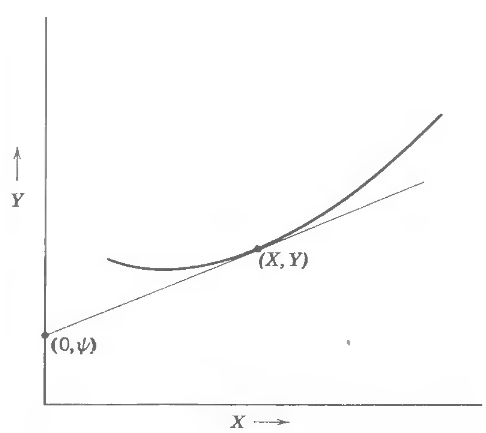
\includegraphics[width=.7\textwidth]{fig5.6.png}
	\figcaption{}
	\label{fig5.6}
}

现在的问题是给出关系$Y=Y(X)$后如何计算$\psi=\psi(P)$。相应的数学操作称为Legendre变换。考虑一条经过点$(X,Y)$,斜率为$P$的切线。如果截距是$\psi$,则有(见图\ref{fig5.6})
\begin{equation}
\label{equ5.19}
	P=\frac{Y-\psi}{X-0}
\end{equation}
或者
\begin{equation}
\label{equ5.20}
	\psi=Y-PX
\end{equation}

基本方程已经给出:
\begin{equation}
\label{equ5.21}
	Y=Y(X)
\end{equation}
并且通过求导可以得到
\begin{equation}
\label{equ5.22}
	P=P(X)
\end{equation}
于是联立方程\eqref{equ5.20}、\eqref{equ5.21}和\eqref{equ5.22}消去%
\footnote{只有在$P$与$X$有关(也就是$\rd^2 Y / \rd X^2 \neq 0$)的情况下才能消去$X, Y$,这在热力学对应于稳定性的要求。这个条件只有在“临界点”才会失效,相关内容在第\ref{chap10}章讨论。}%
$X$和$Y$我们就能得到想要的$\psi$和$P$之间的关系。Legendre变换的基本等式就是方程\eqref{equ5.20},而这个方程可以当成函数$\psi$的解析定义。函数$\psi$称为$Y$的{\it Legendre变换(Legendre transformation)}。

相反的问题是给出关系$\psi=\psi(P)$,重新求出关系$Y=Y(X)$。可以看出$(X,Y)$和$(\psi,P)$之间的关系跟它的逆关系是对称的,区别只是Legendre的方程中差了一个负号。
对方程\eqref{equ5.20}求导并且应用$\,\mathrm dY=P\,\mathrm dX$可得
\begin{align}
\label{equ5.23}
	\,\mathrm d\psi &= \,\mathrm dY-P\,\mathrm dX-X\,\mathrm dP \nonumber \\
	~ &= -X\,\mathrm dP
\end{align}
也就是
\begin{equation}
\label{equ5.24}
	-X=\frac{\mathrm d\psi}{\mathrm dP}
\end{equation}
如果从给出的方程$\psi=\psi(P)$和方程\eqref{equ5.24}和\eqref{equ5.20}中消去%
\footnote{这样做可能的条件是$\rd^2\psi/\rd P^2\neq0$,在热力学中是由所考虑系统的稳定性保证的。}%
两个变量$\psi$和$P$,我们就重构出了关系$Y=Y(X)$。Legendre变换与其逆的对称性可以通过下表对比看出:

{{\centering
\begin{equation*}
\begin{array}{c|c}
\hline
Y=Y(X) & \psi=\psi(P) \\
P=\dfrac{\mathrm dY}{\mathrm dX} & -X=\dfrac{\mathrm d\psi}{\mathrm dP} \\
\psi=-PX+Y & Y=XP+\psi \\
\text{消掉$X$和$Y$得到} & \text{消掉$P$和$\psi$得到} \\
\psi=\psi(P) & Y=Y(X)\\
\hline
\end{array}
\end{equation*}
}}

容易将Legendre变换推广到不止一个独立变量的函数。在三维中,$Y$是关于$X_0$和$X_1$的函数,基本方程表示一个曲面。这个曲面可以当成满足基本方程$Y=Y(X_0,X_1)$的点的轨迹,或者当成切平面的包络面。一个平面可以用在在$Y$轴上的截距$\psi$和在$Y-X_0$以及$Y-X_1$平面上的截线的斜率$P_0$和$P_1$来刻画。于是基本方程就是所有可能的平面中用$\psi=\psi(P_0,P_1)$描述的子集。

基本方程的一般形式
\begin{equation}
\label{equ5.25}
	Y=Y(X_0,X_1,\dots,X_t)
\end{equation}
表示了一个在直角坐标$Y,X_0,X_1,\dots,X_t$的$(t+2)$维空间中的超平面。导数
\begin{equation}
\label{equ5.26}
	P_k=\frac{\partial Y}{\partial X_k}
\end{equation}
是曲面的偏斜率。超曲面可以等价地用满足方程\eqref{equ5.25}描述的点的轨迹或者切超平面的包络来描述。切超平面族可以用超平面的截距$\psi$关于斜率$P_0,P_1,\dots,P_t$的函数来刻画。
于是
\begin{equation}
\label{equ5.27}
	\psi=Y-\sum_kP_kX_k
\end{equation}
对上式微分可得
\begin{equation}
\label{equ5.28}
	\,\mathrm d\psi=-\sum_kX_k\,\mathrm dP_k
\end{equation}
从而
\begin{equation}
\label{equ5.29}
	-X_k = \frac{\partial \psi}{\partial P_k}
\end{equation}
Legendre变换实现了从$Y=Y(X_0,X_1,\dots,X_t)$、方程组\eqref{equ5.26}和方程\eqref{equ5.27}中消去$Y$和$X_k$。逆变换实现了从$\psi=\psi(P_0,P_1,\dots,P_r)$、方程组\eqref{equ5.29}和方程\eqref{equ5.27}中消去$Y$和$X_k$。

最后,Legendre变换可以仅仅在关系$Y=Y(X_0,X_1,\dots,X_t)$的$(t+2)$维全空间中的一个$(n+2)$维子空间中进行。显然这个子空间必须包含$Y$坐标,但是可以包含集合$X_0,X_1,\dots,X_t$中的任选$n+1$个坐标。为了记号上的方便,我们排列坐标使得Legendre变换作用在前$n+1$个坐标(以及$Y$)构成的子空间上;坐标$X_{n+1},X_{n+2},\dots,X_t$保持不变。这样一个部分Legendre变换的作用只不过是在变换中把$X_{n+1},X_{n+2},\dots,X_t$当成常数。这样的Legendre变换必须用符号标出哪些独立变量参与了变换。我们引入标记$Y[P_0,P_1,\dots,P_n]$来标记对函数$Y(X_0,X_1,\dots,X_t)$做对应于$X_0,X_1,\dots,X_n$的Legendre变换。从而$Y[P_0,P_1,\dots,P_n]$就是一个关于独立变量$P_0,P_1,\dots,P_n,X_{n+1},\dots,X_t$的函数。
在接下来的表中展示了在部分Legendre变换和它的逆变换中包含的各种关系。

\begin{tabularx}{1.4\textwidth}{X|X}
\hline
  $Y=Y(X_0,X_1,\dots,X_t)$ & \begin{mymath}Y[P_0, P_1, \dots, P_n] = P_0, P_1, \dots, P_n, X_{n+1}, \dots, X_t \, \text{的函数}\label{equ5.30}\end{mymath}\\
  $P_k = \frac{\partial Y}{\partial X_k}$ & \begin{mymath}-X_k = \frac{\partial Y[P_0,\dots,P_n]}{\partial P_k}, \quad k\leq n\label{equ5.31}\end{mymath} \\
   & $P_k = \frac{\partial Y[P_0,\dots,P_n]}{\partial X_k}\quad k > n$ \\
  求偏导数过程中除了$X_k$之外所有$j\neq k$的$X_j$都不变 & 求偏导数过程中其他自然变量都不变 \\
  $\,\mathrm dY=\sum_0^t P_k\,\mathrm dX_k$ & \begin{mymath}\mathrm dY[P_0, \dots, P_n] = -\sum_0^n X_k \,\mathrm dP_k + \sum_{n + 1}^t P_k \,\mathrm dX_k \label{equ5.32}\end{mymath}\\
  $Y[P_0,\dots,P_n]=Y-\sum_0^nP_kX_k$ & \begin{mymath}Y=Y[P_0,\dots,P_n]+\sum_0^nX_kP_k\label{equ5.33}\end{mymath} \\
  从方程(5.30),(5.33)和(5.31)的前$n+1$个方程中消除掉$Y$和$X_0, X_1,\dots,X_n$可以导出变换后的基本关系。 & 从方程(5.30),(5.33)和(5.31)的前$n+1$个方程中消除掉$Y[P_0, \dots, P_n]$和$P_0, P_1, \dots, P_n$可以导出原始的基本关系。\\
  \hline
\end{tabularx}



本节讲述了Legendre变换的数学形式,而未涉及其物理应用。在介绍热力学的应用之前,我们指出它在物理学中相比热力学更为人熟知的一个领域——Lagrangian和Hamiltonian力学中的应用。Lagrange原理宣称,存在一个特殊的函数Lagrangian\mpar{通译为“拉格朗日量”或简称“拉氏量”,本书英文人名一律不译。},完整刻画了一个力学系统的动力学。Lagrangian是一个关于$2r$个变量的函数,其中$r$个是{\it 广义坐标(generalized coordinates)},$r$个是{\it 广义速度(generalized velocities)}。因此方程
\begin{equation}
\label{equ5.34}
	L=L(v_1,v_2,\dots,v_r,q_1,q_2,\dots,q_r)
\end{equation}
扮演了基本关系的角色。

{\it 广义动量(generalized momenta)}定义成Lagrangian的导数
\begin{equation}
\label{equ5.35}
	P_k \equiv \frac{\partial L}{\partial v_k}
\end{equation}
如果想要用动量代替速度作为独立变量,我们必须做关于速度的部分Legendre变换。
从而我们引入一个新的函数,叫做Hamiltonian\mpar{通译为“哈密顿量” \sout{越来越多的人采用“蛤密顿量”以纪念长者},本书英文人名一律不译。},定义是%
\footnote{我们约定Lagrangian的Legendre变换是{\it 负}的Hamiltonian。实际上,数学上的约定和力学中的是一样的,而函数$-\psi$会被叫做$Y$的Legendre变换}%
\begin{equation}
\label{equ5.36}
	(-H)=L-\sum_{k = 1}^r P_kv_k
\end{equation}
然后一个完整的动力学形式就可以基于这个新的基本关系给出
\begin{equation}
\label{equ5.37}
  H=H(P_1,P_2,\dots,P_r,q_1,q_2,\dots,q_r)
\end{equation}
此外,根据方程(5.31), $H$的关于$P_k$的导数是速度$v_k$,也就是Hamilton动力学方程之一。因此如果形如\eqref{equ5.34}式的一个方程被当成Lagrangian力学的动力学方程,那么Hamilton方程\eqref{equ5.37}就是Hamiltonian力学中等价的基本方程。

\subsection*{习题}

\section{热力学势}
\label{sec5.3}
前面介绍的形式在热力学中的应用是不言自明的。基本关系$Y=Y(X_0,X_1,\dots)$可以解释为能量表象的基本关系$U=U(S,X_1,X_2,\dots,X_t)$或者$U=U(S,V,N_1,N_2,\dots)$。而偏导数$P_0,P_1,\dots$对应着强度量$T,-P,\mu_1,\mu_2,\dots$。
Legendre变换后的函数叫做{\it 热力学势},而现在我们明确定义它们中最常见的几个。在第\ref{chap6}章中将通过每一个势的极值原理继续关于这些函数的讨论,表明每一个的直观意义,并且讨论在热力学理论中它们的特殊角色。但下面只关注几个特定的函数的形式化定义。

{\it Helmholtz势(Helmholtz potential)}或者{\it Helmholtz自由能(Helmholtz free energy)},是$U$用温度代替熵成为独立变量的Legendre变换得到的。按国际标准,Helmholtz势的符号是$F$。Helmholtz势的自然变量是$T,V,N_1,N_2,\dots$。
也就是函数关系$F=F(T,V,N_1,N_2,\dots)$构成一个基本关系。按\ref{sec5.2}节规定的记号:
\begin{equation}
\label{equ5.38}
	F\equiv U[T]
\end{equation}

能量表象和Helmholtz表象的完整关系总结在了下面的对比表中:

\begin{tabular}{c|c}
\hline
$U=U(S,V,N_1,N_2,\dots)$ & \begin{mymath}F=F(T,V,N_1,N_2,\dots)\label{equ5.39}\end{mymath}\\
$T=\partial U/\partial S$ & \begin{mymath}-S=\partial F/\partial T\label{equ5.40} \end{mymath}\\
$F=U-TS$ & \begin{mymath}U=F+TS \label{equ5.41} \end{mymath}\\
消去$U$和$S$得到 & 消去$F$和$T$得到\\
$F=F(T,V,N_1,N_2,\dots)$ & $U=U(S,V,N_1,N_2,\dots)$\\
\hline
\end{tabular}

全微分$\mathrm dF$是
\begin{equation}
\label{equ5.42}
  \,\mathrm dF=-S\,\mathrm dT-P\,\mathrm dV+\mu_1\,\mathrm dN_1+\mu_2\,\mathrm dN_2+\cdots
\end{equation}

{\it 焓(enthalpy)}是$U$用压强代替体积成为独立变量的Legendre变换得到的。按照国际物理学会和化学学会的建议,以及与基本\sout{用}法保持一致,我们用符号$H$来标记焓。这个势的自然变量是$S,P,N_1,N_2,\dots$,
\begin{equation}
\label{equ5.43}
	H\equiv U[P]
\end{equation}
能量表象和焓表象的关系表如下:

\begin{tabular}{c|c}
\hline
$U=U(S,V,N_1,N_2,\dots)$ & \begin{mymath}H=H(S,P,N_1,N_2,\dots)\label{equ5.44}\end{mymath}\\
$-P=\partial U/\partial V$ & \begin{mymath}V=\partial H/\partial P\label{equ5.45} \end{mymath}\\
$H=U+PV$ & \begin{mymath}U=H-PV \label{equ5.46} \end{mymath}\\
\text{消去$U$和$V$得到} & \text{消去$H$和$P$得到}\\
$H=H(S,P,N_1,N_2,\dots)$ & $U=U(S,V,N_1,N_2,\dots)$\\
\hline
\end{tabular}

需要特别注意的是方程(5.45)和(5.46)的正负不同,这是由于$-P$是对应于$V$的强度量。

全微分$\mathrm dH$是
\begin{equation}
\label{equ5.47}
	\mathrm dH=T\,\mathrm dS+V\,\mathrm dP+\mu_1\,\mathrm dN_1+\mu_2\,\mathrm dN_2+\dots
\end{equation}

第三个常用的能量的Legendre变换是{\it Gibbs势(Gibbs potential)},或者叫{\it Gibbs自由能(Gibbs free energy)}。这个势是同时用温度代替熵并用压强代替体积作为独立变量的Legendre变换。标准的记号是$G$,而自然变量是$T,P,N_1,N_2,\dots$。
从而有
\begin{equation}
\label{equ5.48}
  G\equiv U[T,P]
\end{equation}
以及

\begin{tabular}{c|c}
\hline
$U=U(S,V,N_1,N_2,\dots)$ & \begin{mymath}G=G(T,P,N_1,N_2,\dots)\label{equ5.49}\end{mymath}\\
$T=\partial U/\partial S$ & \begin{mymath}-S=\partial G/\partial T\label{equ5.50} \end{mymath}\\
$-P=\partial U/\partial V$ & \begin{mymath}V=\partial G/\partial P\label{equ5.51} \end{mymath}\\
$G=U-TS+PV$ & \begin{mymath}U=G+TS-PV \label{equ5.52} \end{mymath}\\
消去$U$,$S$和$V$得到 & 消去$G$,$T$和$P$得到\\
$G=G(T,P,N_1,N_2,\dots)$ & $U=U(S,V,N_1,N_2,\dots)$\\
\hline
\end{tabular}

全微分$\mathrm dG$是
\begin{equation}
\label{equ5.53}
	\,\mathrm dG=-S\,\mathrm dT+V\,\mathrm dP+\mu_1\,\mathrm dN_1+\mu_2\,\mathrm dN_2+\dots
\end{equation}

{\it 巨正则势}$U[T,\mu]$是在统计力学中自然出现的热力学势,对于这个势有:

\begin{tabular}{c|c}
\hline
$U=U(S,V,N)$ & \begin{mymath}U[T,\mu]=T,V,\text{和}\mu\text{的函数}\label{equ5.54}\end{mymath}\\
$T=\partial U/\partial S$ & \begin{mymath}-S=\partial U[T,\mu]/\partial T\label{equ5.55} \end{mymath}\\
$\mu=\partial U/\partial N$ & \begin{mymath}-N=\partial U[T,\mu]/\partial\mu\label{equ5.56} \end{mymath}\\
$U[T,\mu]=U-TS-\mu N$ & \begin{mymath}U=U[T,\mu]+TS+\mu N \label{equ5.57} \end{mymath}\\
消去$U$,$S$和$N$得到 & 消去$U[T,\mu]$,$T$和$P$得到\\
$T,V,\mu$的函数$U[T,\mu]$ & $U=U(S,V,N)$\\
\hline
\end{tabular}

以及
\begin{equation}
\mathrm dU[T,\mu] = -S\,\mathrm dT -P\,\mathrm dV-N\,\mathrm d\mu
\label{equ5.58}
\end{equation}

简单系统内能$U$的其他可能的Legendre变换,如$U[\mu_1]$,$U[P,\mu_1]$,$U[T,\mu_1,\mu_2]$等等,由于不常用而没有通用的命名。完全的Legendre变换是$U[T,P,\mu_1,\mu_2,\dots,\mu_r]$,$U(S,V,N_1,N_2,\dots,N_t)$是它自变量的一阶齐次函数,这导致了$U[T,P,\mu_1,\mu_2,\dots,\mu_r]$恒等于0:

对于
\begin{equation}
\label{equ5.59}
	U[T,P,\mu_1,\mu_2,\dots,\mu_r]=U-TS+PV-\mu_1N_1-\mu_2N_2-\cdots-\mu_rN_r
\end{equation}
根据Euler关系\eqref{equ3.6}式,上式恒等于零:
\begin{equation}
\label{equ5.60}
	U[T,P,\mu_1,\mu_2,\dots,\mu_r]\equiv 0
\end{equation}

\subsection*{习题}

\section{推广的Massieu函数}
\label{sec5.4}
Legendre变换定义的最常用的函数就是\ref{sec5.3}节中提到的那些,此外可以对熵而不是能量做Legendre变换。也就是形如$S=S(U,V,N_1,N_2,\dots)$的基本关系可以当成变换作用的关系。这种对熵的Legendre变换是1869年Massieu发明的,并且提前得到了Gibbs在1875年引入的对能量的变换。
我们把对于熵的变换叫做{\it Massieu函数(Massieu functions)},用来跟从能量变换得到的{\it 热力学势(thermodynamics potentials)}做出区分。
Massieu函数在不可逆热力学的理论中会特别有用,并且在统计力学以及热涨落理论中会自然出现。
三个典型的Massieu函数包括$S[1/T]$,其中温度的倒数代替能量成为了独立变量;$S[P/T]$,其中$P/T$代替体积成为了独立变量;以及$S[1/T,P/T]$,两个替换同时进行。显然
\begin{equation}
\label{equ5.61}\
  S\left[\frac{1}{T}\right]\equiv S-\frac{1}{T}U=-\frac{F}{T}
\end{equation}
\begin{equation}
\label{equ5.62}\
  S\left[\frac{P}{T}\right]\equiv S-\frac{P}{T}\cdot V
\end{equation}
以及
\begin{equation}
\label{equ5.63}\
  S\left[\frac{1}{T},\frac{P}{T}\right]\equiv S-\frac{1}{T}U-\frac{P}{T}\cdot V=-\frac{G}{T}
\end{equation}
从而,这三个中只有$S[P/T]$是不平凡地依赖于前面介绍过的某一个热力学势的。
对于这个函数有:

\begin{tabular}{c|c}
\hline
$S=S(U,V,N_1,N_2,\dots) $& \begin{mymath}S[P/T]=U,P/T,N_1,N_2\text{的函数}\label{equ5.64}\end{mymath}\\
$P/T=\partial S/\partial V $& \begin{mymath}-V=\partial S[P/T]/\partial(P/T)\label{equ5.65} \end{mymath}\\
$S[P/T]=S-(P/T)V $& \begin{mymath}S=S[P/T]+(P/T)V \label{equ5.66} \end{mymath}\\
消去$S$和$V$得到 & 消去$S[P/T]$和$P/T$得到\\
$U,P/T,N_1,N_2,\dots$的函数$S[P/T]$ & $S=S(U,V,N_1,N_2,\dots)$ \\
\hline
\end{tabular}

以及
\begin{equation}
\label{equ5.67}
	\rd S[P/T]=(1/T) \rd U-V \rd (P/T)-(\mu_1/T) \rd N_1-(\mu_2/T) \rd N_2\dots
\end{equation}
其它的Massieu函数可以在读者在特殊情况下用到它们时自己定义和分析。

\subsection*{习题}

\chapter{Legender变换表象中的极值原理}
\label{chap6}

\section{Helmholtz势}
\label{sec6.2}

对于一个与热库有热接触的复合系统,其平衡态使得等温态(与热库的温度相等)流形上的Helmholtz势最小。
事实上很多过程都在有着透热壁的刚性容器中发生,比方说环境大气可以视为一个热库,对于这些情况Helmholtz势表象是相当合适的。\mpar{原文:{In practice many processes are carried out in rigid vessels with diathermal walls, so that the ambient atmosphere acts as a thermal reservoir; for these the Helmholtz potential representation is admirably suited.}}

 Helmholtz势函数是以$T$,$V$,$N_1$,$N_2$,…为自变量的自然函数(natural function)。
$T$为常数的条件减少了这个问题中变量的数量,使得$F$成为一个只与变量$V$,$N_1$,$N_2$,…有关的函数。
这与$T$的固定在能量表象中体现出的行为形成了鲜明的对比。具体来说,在能量表象中$U$是$S$,$V$,$N_1$,$N_2$,…的函数,但附加条件$T=T^r$暗示着这些变量间的一个关系。
特别地,在对状态方程$T=T(S, V, N)$的具体形式一无所知的情况下,这个附加的限制将导致能量表象中的解析过程无从下手。

作为Helmholtz势用途的一个例证我们先考虑一个复合系统,这个复合系统由两个被一个可移动的、绝热的、不可透过的壁(例如一个刚性绝热活塞)隔开的简单系统组成。
这两个子系统每一个都与温度$T^r$的热库之间有热接触。
问题是预测两个子系统的体积$V^{(1)}$和$V^{(2)}$。
我们有
\begin{equation}
\label{equ6.23}
P^{(1)}\left(T^r, V^{(1)}, N_1^{(1)}, N_2^{(1)}, ...\right)=P^{(2)}\left(T^r, V^{(2)}, N_1^{(2)}, N_2^{(2)}, ...\right)
\end{equation}
这是一个包含两个变量$V^{(1)}$和$V^{(2)}$的方程;所有其余量都是常数。封闭条件
\begin{equation}
\label{equ6.24}
V^{(1)}+V^{(2)}=V
\end{equation}
提供了另一个需要的方程,使得$V^{(1)}$与$V^{(2)}$可以被明确解出。

在能量表象中我们亦能发现压强相等,正如在方程$6.23$中那样,但此时压强是熵、体积、摩尔数的函数。
我们将需要状态方程来把熵同温度与体积联系在一起;$6.23$与$6.24$两个同时存在的方程将变成$4$个。

尽管这种从$4$个方程到$2$个的简化也许看起来仅仅是个微小的成功,在更加复杂的情形下这种简化将带来巨大的方便。
也许关于这个概念的更加大价值是Helmholtz表象让我们将我们的思考过程没有干扰地集中在我们感兴趣的子系统上,与此同时只把热库视为一个隐含的角色。
最后,由于数学技巧上的原因(这将在第$16$章中详细讲到),在Helmholtz表象下统计力学的计算将被巨大地简化,使得难以对付的计算成为可能。

对于一个与热库有接触的系统,Helmholtz势可以被解释为一定温度下可获得的功。考虑一个与热库有热接触的系统,它与一个可逆功源(reversible work source)之间有相互作用。在一个可逆过程中给可逆功源(reversible work source)输入的功与系统减少的能量相等,并且
\begin{align}
\label{equ6.25}
dW_{RWS}&=-dU-dU'=-dU-T^rdS^r \\
\label{equ6.26}
                  &=-dU+T^rdS=-d(U-T^rS) \\
\label{equ6.27}
                  &=-dF
\end{align}
因此在一个可逆过程中一个与热库有接触的系统所释放的能量与这个系统Helmholtz势减少的量相等。
Helmholtz势经常被称作Helmholtz自由能,尽管短语“一定温度下可获得的功”更不容易被误解。

\subsection*{例子1}
一个圆筒内部包含一个活塞,活塞的每一侧都有一摩尔的单原子分子理想气体。
圆筒的壁是透热的,整个系统浸入到一个温度在$0$摄氏度的大液浴(一个热库)中。
这两个气体子系统(活塞的两边)的初始体积分别为$10$升和$1$升。
活塞现在被可逆地移动,使得其两边最后的体积分别为$6$升和$5$升。
问做了多少功?
\subsubsection*{答案}
正如在问题$5.3-1$中读者见到的那样,Helmholtz势表象中单原子分子理想气体的基本方程式为
\begin{equation}
\notag
F=NRT\left\{\frac{F_0}{N_0RT_0}-ln\left[\left(\frac{T}{T_0}\right)^{3/2}\frac{V}{V_0}\left(\frac{N}{N_0}\right)\right]\right\}
\end{equation}
当$T$与$N$为常数时这意味着
\begin{equation}
\notag
F=常数-NRTlnV
\end{equation}
Helmholtz势的变化为
\begin{equation}
\notag
\Delta F=-NRT[ln6+ln5-ln10-ln1]=-NRTln3=-2.5kJ
\end{equation}
因此$2.5kJ$的功被用于这个过程。

在这里注意到一件有趣的事情,所有的能量都来自于热库。
单原子分子理想气体的能量仅仅是$\frac{3}{2}NRT$,因此它在一定的温度下是个常数。
然而,我们从热库中吸取能量并将它作为注入到可逆功源的功的事实并不违反Carnot效率原理,因为气体子系统并不处在它们的初始态上。
除了这些子系统的能量保持恒定的事实外,它们的熵增加了。

%!TEX root = ../CallenThermo.tex
% 翻译:SI
% 未校对!

\chapter{Maxwell关系}
\label{chap7}

\section{Maxwell关系}
\label{sec7.1}
\ref{sec3.9}节\mpar{原文为\ref{sec3.6}节,根据内容来看应该是\ref{sec3.9}节。这里进行了修改。}讨论了绝热压缩率、热膨胀系数、摩尔热容等热力学量的物理意义。它们都具有$(\partial X / \partial Y)_{Z, W}$的形式,式中字母表示热力学广延量或强度量。一般的热力学系统有许多热力学量,从而可以构造大量这样的导数。但是众多的导数量之间存在羁绊,由此其中只有一小部分是独立的,其余的量可以用这一小部分表示。自然,这些关系可以大大简化热力学分析。并且我们不需要特意记忆公式\mpar{比如“{\bf G}ood {\bf P}hysicists {\bf H}ave {\bf S}tudied {\bf U}nder {\bf V}ery {\bf F}ine {\bf T}eachers”什么的……\sout{来自热统课的惨痛回忆}\ \sout{\ref{sec7.2}节有首字母相同的另一句话} }。 下面介绍在热力学计算过程中用到的简单、直接推导这些关系的方法,也就是本章的主题。

首先说明这些导数量之间“羁绊”的存在性,考虑\eqref{equ3.70}与\eqref{equ3.71}式:
\begin{align}
	\frac{\partial^2 U}{\partial S \partial V} &= \frac{\partial^2 U}{\partial V \partial S}, \label{equ7.1} \\
	-\left( \frac{\partial P}{\partial S} \right)_{V, N_1, N_2} &= \left( \frac{\partial T}{\partial V} \right)_{S, N_1, N_2}. \label{equ7.2}
\end{align}
上式是导数量的“羁绊”——称为{\it Maxwell 关系 (Maxwell relations)}——的源头,亦即,导数量之间的依赖关系源自基本方程(在不同表象下)的混合导数不依赖于求导次序。

某一热力学量依赖于$(t + 1)$个自变量,从而有$t(t + 1)/2$种不同的混合偏导数,因此每一热力学量对应$t(t + 1)/2 = 3$个Maxwell关系。

单组分简单系统的内能的自变量有$3$个,即$t = 2$,从而有$(2 \cdot 3)/2$个混合偏导数:
\[
	\frac{\partial^2 U}{\partial S \partial V} = \frac{\partial^2 U}{\partial V \partial S}, \quad \frac{\partial^2 U}{\partial S \partial N} = \frac{\partial^2 U}{\partial N \partial S}, \quad \frac{\partial^2 U}{\partial V \partial N} = \frac{\partial^2 U}{\partial N \partial V}.
\]
单组分简单系统的Maxwell列成下表。其中第一列是混合求导的热力学量,第二列是混合求导对应的两个(独立)自变量,第三列是相应的Maxwell关系。\ref{sec7.2}节提供了一种辅助记忆这些关系的图像法。\ref{sec7.3}节举例说明如何利用这些关系解决热力学问题。

\begin{align}
	&U \quad &S, V \quad & \left( \frac{\partial T}{\partial V} \right)_{S, N} =& -\left( \frac{\partial P}{\partial S} \right)_{V, N} \label{equ7.3} \\
	&\,\mathrm dU = T\,\mathrm dS - P\,\mathrm dV + \mu \,\mathrm dN \quad & S, N \quad & \left( \frac{\partial T}{\partial N} \right)_{S, V} =& \left( \frac{\partial \mu}{\partial S} \right)_{V, N} \label{equ7.4} \\
	&\phantom{dU = TdS - PdV + \mu dN \quad} & V, N \quad & -\left( \frac{\partial P}{\partial N} \right)_{S, V} &= \left( \frac{\partial \mu}{\partial V} \right)_{S, N} \label{equ7.5}
\end{align}
————————————————————————————————
\begin{align}
	&U[T]\equiv F & T, V \quad & \left(\frac{\partial S}{\partial V} \right)_{T, N} &= \left( \frac{\partial P}{\partial T} \right)_{V, N} \label{equ7.6} \\
	&\,\mathrm dF = -S\,\mathrm dT - P\,\mathrm dV + \mu \,\mathrm dN \quad & T, N \quad & -\left(\frac{\partial S}{\partial N}\right)_{T, V} &= \left(\frac{\partial \mu}{\partial T} \right)_{V, N} \label{equ7.7} \\
	&\phantom{dF = -SdT - PdV + \mu dN \quad} & V, N \quad & -\left( \frac{\partial P}{\partial N} \right)_{T, V} &= \left( \frac{\partial \mu}{\partial V} \right)_{T, N} \label{equ7.8}
\end{align}
————————————————————————————————
\begin{align}
	& U[P] \equiv H \quad & S, P \quad & \left( \frac{\partial T}{\partial P} \right)_{S, N} &= \left( \frac{\partial V}{\partial S} \right)_{P, N} \label{equ7.9} \\
	&dH = TdS + VdP + \mu dN \quad & S, N \quad & \left( \frac{\partial T}{\partial N} \right)_{S, P} &= \left( \frac{\partial \mu}{\partial S} \right)_{P, N} \label{equ7.10} \\
	&\phantom{\,\mathrm dH = T\,\mathrm dS + V\,\mathrm dP + \mu \,\mathrm dN \quad} & P, N \quad & \left(\frac{\partial V}{\partial N} \right)_{S, P} &= \left( \frac{\partial \mu}{\partial P} \right)_{S, N} \label{equ7.11} 
\end{align}
————————————————————————————————
\begin{align}
	& U[\mu] \quad & S, V \quad & \left(\frac{\partial T}{\partial V} \right)_{S, \mu} &= -\left( \frac{\partial P}{\partial S} \right)_{V, \mu} \label{equ7.12} \\
	& dU[\mu] = TdS - PdV - Nd\mu \quad & S, \mu \quad & \left(\frac{\partial T}{\partial \mu} \right)_{S, V} &= -\left( \frac{\partial N}{\partial S} \right)_{V, \mu} \label{equ7.13} \\
	& \phantom{\,\mathrm dU[\mu] = T\,\mathrm dS - P\,\mathrm dV - N\,\mathrm d\mu \quad} & V, \mu \quad & \left(\frac{\partial P}{\partial \mu} \right)_{S, V} &= \left( \frac{\partial N}{\partial V} \right)_{S, \mu} \label{equ7.14}
\end{align}
————————————————————————————————
\begin{align}
	& U[T, P] \equiv G \quad & T, P \quad & -\left( \frac{\partial S}{\partial P} \right)_{T, N} &= \left( \frac{\partial V}{\partial T} \right)_{P, N} \label{equ7.15} \\
	& \,\mathrm dG = -S\,\mathrm dT + V\,\mathrm dP + \mu \,\mathrm dN \quad & T, N \quad & -\left( \frac{\partial S}{\partial N} \right)_{T, P} &= \left( \frac{\partial \mu}{\partial T} \right)_{P, N} \label{equ7.16} \\
	& \phantom{dG = -SdT + VdP + \mu dN \quad} & P, N \quad & \left( \frac{\partial V}{\partial N} \right)_{T, P} &= \left( \frac{\partial \mu}{\partial P} \right)_{T, N} \label{equ7.17}
\end{align}
————————————————————————————————
\begin{align}
	& U[T, \mu] \quad & T, V \quad & \left( \frac{\partial S}{\partial V} \right)_{T, \mu} &= \left( \frac{\partial P}{\partial T} \right)_{V, \mu} \label{equ7.18} \\
	& dU[T, \mu] = -SdT - PdV - Nd\mu \quad & T, \mu \quad & \left( \frac{\partial S}{\partial \mu} \right)_{T, V} &= \left( \frac{\partial N}{\partial T} \right)_{V, \mu} \label{equ7.19} \\
	& \phantom{dU[T, \mu] = -SdT - PdV - Nd\mu \quad} & V, \mu \quad & \left( \frac{\partial P}{\partial \mu} \right)_{T, V} &= \left( \frac{\partial N}{\partial V} \right)_{T, \mu} \label{equ7.20}
\end{align}
————————————————————————————————
\begin{align}
	& U[P, \mu] \quad & S, P \quad & \left( \frac{\partial T}{\partial P} \right)_{S, \mu} =& \left( \frac{\partial V}{\partial S} \right)_{P, \mu} \label{equ7.21} \\
	& \,\mathrm dU[P, \mu] = T\,\mathrm dS + V\,\mathrm dP + N\,\mathrm d\mu \quad & S, \mu \quad & \left( \frac{\partial T}{\partial \mu} \right)_{S, P} =& -\left( \frac{\partial N}{\partial S} \right)_{P, \mu} \label{equ7.22} \\
	& \phantom{ dU[P, \mu] = TdS + VdP + Nd\mu \quad} & P, \mu \quad & \left( \frac{\partial V}{\partial \mu} \right)_{S, P} =& -\left( \frac{\partial N}{\partial P} \right)_{S, \mu} \label{equ7.23}
\end{align}
————————————————————————————————

\section{Maxwell关系的辅助记忆图}
\label{sec7.2}
最常用的Maxwell关系可以通过如下的图像辅助记忆\footnote{这幅图首次展现于1929年Max Born 所作的一场报告中,由 Tisza教授所记录. 它也出现在论文 F. O. Koenig, {\it J. Chem. Phys} {\bf 3}, 29 (1935),  以及 {\bf 56}, 4556 (1972). 另外可见 L T. Klauder,  {\it Am. Journ. Phys}. {\bf 36}, 556 (1968), 并且此期刊中有其他作者提出的一系列变体。},见图\ref{fig7.1}。它由一个正方形以及两条沿对角线指向上的箭头组成。正方形的每条边由热力学量$F, G, H, U$标记,Helmholtz势$F$居最上,其余三者按顺时针方向的字母表顺序排列。左侧的两个顶点是广延量$V, S$, 右侧顶点是强度量$T, P$. (整个顺序可以用`` {\bf V}alid {\bf F}acts and {\bf T}heoretical {\bf U}nderstanding {\bf G}enerate {\bf S}olutions to {\bf H}ard {\bf P}roblems ''来记忆)

{
	\centering
	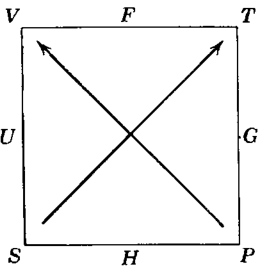
\includegraphics{fig7_1.png}
	\figcaption{热力学正方形}
	\label{fig7.1}
}

位于正方形边上的四个热力学势是它们附近的两个独立变量的函数。例如$U$是$V, S$的函数;$F$是$V, T$的函数;$G$是$T, P$的函数;等等。所有热力学势还是摩尔数$N$的函数,这在图中并未显示。

各热力学势的微分表达式中每一项的正负号由对角线箭头辅助记忆。如果箭头背离自变量,则该项是正的;而箭头指向自变量则表明该项为负。结合如下等式观察图像不难掌握这一方法:
\begin{align}
	\,\mathrm dU &= T\,\mathrm dS - P\,\mathrm dV + \sum_k \mu_k \,\mathrm dN_k \label{equ7.24} \\
	\,\mathrm dF &= -S\,\mathrm dT - P\,\mathrm dV + \sum_k \mu_k \,\mathrm dN_k \label{equ7.25} \\
	\,\mathrm dG &= -S\,\mathrm dT + V\,\mathrm dP + \sum_k \mu_k \,\mathrm dN_k  \label{equ7.26} \\
	\,\mathrm dH &= T\,\mathrm dS + V\,\mathrm dP + \sum_k \mu_k \,\mathrm dN_k  \label{equ7.27}
\end{align}

Maxwell关系可以按如下方法从图中读取。只考虑正方形顶点的量,不难看出等式的图的关系:
\begin{equation}
	\left( \frac{\partial V}{\partial S} \right)_P = \left( \frac{\partial T}{\partial P} \right)_S \quad (N_1, N_2, \dots \text{为常数})
\label{equ7.28}
\end{equation}
{
	\centering
	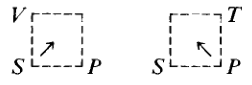
\includegraphics[scale=0.7]{equ7_28.png}
}

把图像顺时针旋转$90^\circ$, 从新图像读出:
\begin{equation}
	\left( \frac{\partial S}{\partial P} \right)_T = -\left( \frac{\partial V}{\partial T} \right)_P \quad (N_1, N_2, \dots \text{为常数})
\label{equ7.29}
\end{equation}
{
	\centering
	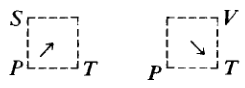
\includegraphics[scale=0.7]{equ7_29.png}
}

上图中两个箭头指向不同意味着上式有负号。再旋转图像两次可以得到其余两个Maxwell关系:
\begin{align}
	\left( \frac{\partial P}{\partial T} \right)_V &= \left( \frac{\partial S}{\partial V} \right)_T \quad (N_1, N_2, \dots, \text{为常数}) \label{equ7.30}\\
	\left( \frac{\partial T}{\partial V} \right)_S &= - \left( \frac{\partial P}{\partial S} \right)_V \quad (N_1, N_2, \dots \text{为常数}) \label{equ7.31}
\end{align}
以上四式即为最常用的Maxwell关系。

这种辅助记忆图还可以推广到变量$S, V$之外的其它变量。例如考虑经Legendre变换后的$S, N_j$, 相应的图像变为\ref{fig7.2}(a). 连接$N_j$与$\mu_j$的箭头与原图中连接$V, P$的箭头方向相反,因为$\mu_j$的地位与$-P$相同。从该图中可以读出\eqref{equ7.4}, \eqref{equ7.7}, \eqref{equ7.13}和\eqref{equ7.19}式。其它Legendre变换的辅助图类似,一般情况见\ref{fig7.2}(b).

{
	\centering
	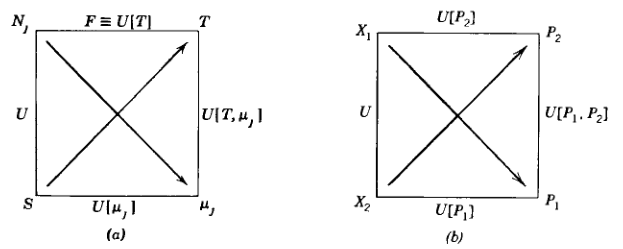
\includegraphics[scale=0.8]{fig7_2.png}
	\figcaption{}
	\label{fig7.2}
}

\subsection*{习题}


\section{单组份系统中一种导数约化的步骤}
\label{sec7.3}
在热力学的实际应用中,经常需要计算特定的偏导数以分析实验过程。例如,分析单组分系统在恒容条件下压强与温度的变化关系,显然有
\begin{equation}
	\rd T = \left( \frac{\partial T}{\partial P} \right)_{V, N} \rd P.
\label{equ7.32}
\end{equation}
然后就是要计算偏导数$(\partial T / \partial P)_{V, N}$. \ref{sec7.4}节会讨论一系列类似问题。这种偏导数量都有共同特点,求导过程中的摩尔数$N$均不变,并且同时含有广延量和强度量。{\it 所有这些导数当中只有三个是独立的,任意选定作为基的三个量之后,其余的偏导数都可以用这三者表示。} 通常选择$c_P, \alpha, \kappa_T$作为基。

$c_P, \alpha, \kappa_T$意味着使用Gibbs表象,因为在该表象下三个量可以用$\partial^2 g / \partial T^2, \partial^2 g / \partial T \partial P$以及$\partial^2 g / \partial P^2$简单表述:它们分别等于$-c_P / T, v\alpha$以及$-v \kappa_T$. 在系统摩尔数不变的情况下,其余的二阶导数都依赖于它们。

{\it 所有一阶导数(既包括对广延量、也包括对强度量求导)可以表为Gibbs势二阶偏导数量的函数,例如上面的$c_P, \alpha, \kappa_T$就构成一组完备集(在摩尔数不变的情况下)。}

“导数约化”的过程原则上十分直接,只需要把熵$S$替换成$-\partial G / \partial T$, $V$换成$\partial G / \partial P$,接着原始偏导数量用$G$对$T, P$的二阶混合导数表示出来即可。但实际上这么干会相当复杂。

学过热力学的人的一个基本技能是熟练掌握“导数约化”技术——将任意偏导数量用已知的偏导数基表示。为此,我们提出一种基于上一节“正方形记忆图”的方法,并且整理成了按部就班的套路。只有进行大量练习才能真正掌握。

以下假设求导过程的摩尔数均不变。要将给定的导数表示为$c_P, \alpha, \kappa_T$的函数。之后会用到如下微分恒等式(见附录A):
\begin{equation}
	\left( \frac{\partial X}{\partial Y} \right)_Z = 1 \Big/ \left(\frac{\partial Y}{\partial X} \right)_Z 
\label{equ7.33}
\end{equation}
以及
\begin{align}
	\left( \frac{\partial X}{\partial Y} \right)_Z &= \left( \frac{\partial X}{\partial W} \right)_Z \Bigg/ \left( \frac{\partial Y}{\partial W} \right)_Z \label{equ7.34} \\
	\left( \frac{\partial X}{\partial Y} \right)_Z &= - \left( \frac{\partial Z}{\partial Y} \right)_X \Bigg/ \left( \frac{\partial Z}{\partial X} \right)_Y \label{equ7.35}
\end{align}

接着,按照顺序执行下列运算:

\begin{enumerate}
\item {\bf 如果导数中含有势函数,那么把它们化到分子中,并且利用热力学正方形包含的等量关系(\eqref{equ7.24} - \eqref{equ7.27}式)将它消去。}
\paragraph{例} 化简导数$(\partial P / \partial U)_{G, N}$.
\begin{align}
	\left( \frac{\partial P}{\partial U} \right)_{G, N} &= \left[ \left( \frac{\partial U}{\partial P} \right)_{G, N} \right]^{-1} \tag{by \eqref{equ7.33} } \\
	&= \left[ T \left( \frac{\partial S}{\partial P} \right)_{G, N} - P \left( \frac{\partial V}{\partial P} \right)_{G, N} \right]^{-1} \tag{by \eqref{equ7.34} }  \\
	&= \left[ -T \left( \frac{\partial G}{\partial P} \right)_{S, N} \Bigg/ \left( \frac{\partial G}{\partial S} \right)_{P, N} + P \left( \frac{\partial G}{\partial P} \right)_{V, N} \Bigg/ \left( \frac{\partial G}{\partial V} \right)_{P, N} \right]^{-1} \tag{by \eqref{equ7.35} } \\
	&= \left[ -T \frac{-S (\partial T / \partial P)_{S, N} + V}{-S (\partial T / \partial S)_{P, N}} + P \frac{-S(\partial T / \partial P)_{V, N} + V}{-S (\partial T / \partial V)_{P, N}} \right]^{-1} \tag{by \eqref{equ7.26} }
\end{align}
经过处理后的表达式不含任何势函数,只含有导数。然后按如下步骤处理导数量。
\item {\bf 如果导数中含有化学势,那么把它化到分子中,再利用Gibbs-Duhem关系}$\rd \mu = -s \,\rd T + v\,\rd P${\it 消去它。}

\paragraph{例} 化简$( \partial \mu / \partial V)_{S, N}$.

\[
	\left( \frac{\partial \mu}{\partial V} \right)_{S, N} = -s \left( \frac{\partial T}{\partial V} \right)_{S, N} + v \left( \frac{\partial P}{\partial V} \right)_{S, N}
\]
\item {\bf 如果导数中含有熵,则将它化到分子。如果正方形记忆图中的四个Maxwell关系可以消去这个熵的导数,则调用它消去。如果Maxwell关系不能消去熵,那么利用\eqref{equ7.34}式(令其中的$w = T$)凑出$\partial S / \partial T$, 这样分子就能表示为热容$c_v$或$c_P$的函数。}

\paragraph{例} 考虑第1步出现的导数$(\partial T / \partial P)_{S, N}$:
\begin{align}
	\left( \frac{\partial T}{\partial P} \right)_{S, N} &= - \left( \frac{\partial S}{\partial P} \right)_{T, N} \Bigg/ \left( \frac{\partial S}{\partial T} \right)_{P, N} \tag{by \eqref{equ7.35}} \\
	&= \left( \frac{\partial V}{\partial T} \right)_{P, N} \Bigg/ \frac{N}{T} c_P \tag{by \eqref{equ7.29}}
\end{align}

\paragraph{例} 考虑导数$(\partial S / \partial V)_{P, N}$, 利用Maxwell关系$(\partial S / \partial V)_{P, N} = (\partial P / \partial T)_{S, N}$ (\eqref{equ7.28}式)不能消去熵,因此不调用Maxwell关系,而是凑出$\partial S / \partial T$:
\begin{equation}
	\left( \frac{\partial S}{\partial V} \right)_{P, N} = \frac{(\partial S / \partial T)_{P, N}}{(\partial V / \partial T)_{P, N}} = \frac{(N / T) c_P}{(\partial V / \partial T)_{P, N}} \tag{by \eqref{equ7.34}}
\end{equation}
于是将导数化成了不含势函数也不含有熵的形式,只包括$V, P, T$(当然还有$N$)。
\item {\bf 将$V$化入分子,这样出现的量都能表示为$\alpha$与$\kappa_T$的函数。}

\paragraph{例} \begin{equation}
	\left( \frac{\partial T}{\partial P} \right)_{V, N} = -\left( \frac{\partial V}{\partial P} \right)_{T, N} \Bigg/ \left( \frac{\partial V}{\partial T} \right)_{P, N} = \frac{\kappa_T}{\alpha} \tag{by \eqref{equ7.35}}
\end{equation}

\item {\bf 最初给定的导数经以上步骤已经化成了用$c_v, c_P, \alpha, \kappa_T$表示的形式。恒容热容可以用下式消去:}
\begin{equation}
	c_v = c_P - \frac{Tv\alpha^2}{\kappa_T}
\label{equ7.36}
\end{equation}
\end{enumerate}

上式即\eqref{equ3.75}式的变形,它经常被用到,应该牢记。读者也要掌握上式的推导(见习题7.3-2)。

上面导数约化的步骤以单组分系统为例,但也可以推广到多组分系统,只要组分的化学势$\mu_j$不出现在导数中(因为单组分系统的化学势是通过Gibbs-Duhem关系消去的,对于多组分系统而言G-D关系将一种化学势化为了其他化学势)。

\subsection*{习题}

\section{简单应用}
\label{sec7.4}
本节介绍\ref{sec7.3}节的几个代表性应用,每个例子以一个问题 —— 研究某一参量在其他参量变化的情况下的变化情况 —— 开始。最简单的情形是简单系统在恒容条件下,温度变化$\Delta T$对应的压强变化$\Delta P$.

我们用两种方法解决该问题。首先,如果基本方程已知,则可以直接求解。第二种方法的条件是已知$c_P, \alpha, \kappa_T$,且各参量的变化为小量。

\subsection*{绝热压缩}
考虑被绝热壁包围的单组分简单系统(粒子数为$N$)。系统的初始温度与压强已知,经准静态压缩后,压强从$P_i$变为$P_f$. 如何得出其他热力学量(如体积、温度、内能、化学势)的变化?

求解的关键在于——绝热壁表明了系统的熵在准静态过程中不变。该判断的依据当然是准静态过程中$\dbar Q = T \rd S$.

以温度为例,计算其变化。首先假设系统的基本方程已知,对它微分可得两个状态方程$T = T(S, V, N)$与$P = P(S, V, N)$. 初始温度与压强已知,于是可得初始体积与熵。联立上两个状态方程消去$V$得到温度$T$关于$S, P, N$的关系式,于是得到温度的变化:
\begin{equation}
	\Delta T = T(S, P_f, N) - T(S, P_i, N)
\label{equ7.37}
\end{equation}

如果基本方程未知,但知道$c_P, \alpha, \kappa_T$,并且压强的变化是小量,则有
\begin{equation}
	\rd T = \left( \frac{\partial T}{\partial P} \right)_{S, N} \rd P 
\label{equ7.38}
\end{equation}
利用\ref{sec7.3}节介绍的套路可以算出
\begin{equation}
	\rd T = \frac{Tv\alpha}{c_P} \rd P 
\label{equ7.39}
\end{equation}

化学势的求解过程相似。答案是(仍然要求压强变化量是小量):
\begin{align}
	\rd \mu &= \left( \frac{\partial \mu}{\partial P} \right)_{S, N} \rd P \label{equ7.40} \\
	&= \left( v - \frac{sTv\alpha}{c_P} \right) \rd P \label{equ7.41}
\end{align}

系统在(无穷小)绝热压缩过程中体积的相对变化由{\it 绝热压缩率}$\kappa_S$表征,定义见$\eqref{equ3.73}$式。那里曾提到过$\kappa_S$可以由$\kappa_T, c_P, \alpha$表示(\eqref{equ3.76}式,又见习题3.9-5),这里建议读者完成习题7.4-8。

\subsection*{等温压缩}
系统在恒温、摩尔数不变的条件下准静态压缩,压强从$P_i$变到$P_f$. 还是要计算$U, S, V, \mu$的变化。通过对基本方程与状态方程一通捣鼓以消去变量,可以得到$U, S, V, \mu$各自关于$T, P, N$的表达式,于是可得各参量的变化。

对于压强的微小变化,有
\begin{align}
	\rd S &= \left( \frac{\partial S}{\partial P} \right)_{T, N} \rd P \label{equ7.42} \\
	&= -\alpha V \rd P \label{equ7.43}
\end{align}
同样也有
\begin{align}
	\rd U &= \left( \frac{\partial U}{\partial P} \right)_{T, N} \rd P \label{equ7.44} \\
	&= ( -T \alpha V + PV \kappa_T) \,\rd P \label{equ7.45}
\end{align}
其他参量同理。

有时需要求出为保持系统在压缩过程保持温度不变而从系统吸收的热量。首先还是假设基本方程已知,于是热量变化为
\begin{equation}
	\Delta Q = T\Delta S = TS(T, P_f, N) - TS(T, P_i, N)
\label{equ7.46}
\end{equation}
其中基本方程$S(U, V, N)$(通过与状态方程联立等等一通折腾)变成了$S(T, P, N)$的形式。 

如果不知道基本方程:首先考虑无穷小的等温压缩过程,由\eqref{equ7.43}式可得
\begin{equation}
	\dbar Q = -T\alpha V \,\rd P 
\label{equ7.47}
\end{equation}
然后是有限大(非无穷小)的等温压缩。注意,基本方程未知,\eqref{equ7.46}式不能用。如果已知$\alpha, V$关于$T, P$的函数,那么对\eqref{equ7.47}式沿等温过程积分就得到热量变化:
\begin{equation}
	\Delta Q = -T \int_{P_i}^{P_f} \alpha V \,\rd P 
\label{equ7.48}
\end{equation}
这个解必然与\eqref{equ7.46}式一致。

\subsection*{自由膨胀}
第三个例子是自由膨胀过程(习题3.4-8, 4.2-3接触过它)。系统的初始体积为$V_i$,突然释放使系统膨胀到体积$V_f$. 如果是气体系统(当然,下面的推导不只针对气体),则该过程可以用如下装置方便地实现:某一刚性容器由隔板分为两部分,一部分是气体,另一部分真空。突然撤去隔板,则气体自发膨胀充满整个容器。系统的其他参量在该过程的变化如何求解?

既然是自由膨胀,则系统的内能不变。系统既未向外传热,也没有对外做功。

如果已知温度关于$U, V, N$的表达式,则有
\begin{equation}
	T_f - T_i = T(U, V_f, N) - T(U, V_i, N)
\label{equ7.49}
\end{equation}
如果体积的变化为小量,则
\begin{align}
	\rd T &= \left( \frac{\partial T}{\partial V} \right)_{U, N} \rd V \label{equ7.50} \\
	&= \left( \frac{P}{N c_v} - \frac{T\alpha}{N c_v \kappa_T} \right) \rd V \label{equ7.51}
\end{align}

与前两例不同,自由膨胀过程本质上既不可逆,也不是准静态的(见习题4.2-3)。
\begin{example}
三次元的真实过程不可能像例子们那样简洁可爱,没有任何参量在演化前后是不变的。例如计算发动机气缸在膨胀冲程(expansion stroke,又称为做功冲程)前后的温度变化,气缸壁可以自由传热,故而该膨胀过程既不等温也不绝热。然而,经验表明温度可以近似表为体积的函数,于是该过程可以用$T = T(V)$定义。读者会遇到许多将真实过程模型化的情况,这个例子可以作为参考。

某一单组分系统(摩尔数$N$)经膨胀过程,体积从$V_1$变为$V_2$,温度从$T_1$降至$T_2$,并且观测到温度随体积线性减少。计算在膨胀过程中外界对系统做的功以及传入系统的热量,答案用$c_P, \alpha, \kappa_T$的表达式或积分表示。

{\bf 求解:}\\
首先注意到函数$c_P (T, P), \alpha(T, P), \kappa_T (T, P)$, 以及$v(T, P)$ (它们可以查表求出)是有冗余的。\ref{sec3.9}的例题已经推导过,从前三个函数可以导出最后一个。

题目里的膨胀过程在$T\text{-}V$图上对应的轨迹为
\begin{align*}
	T &= A + BV; \\
	A &= \frac{T_1 V_2 - T_2 V_1}{V_2 - V_1}; \\
	B &= \frac{T_2 - T_2}{V_2 - V_1}.
\end{align*}
此外,$v(T, P)$可以转化为$P$关于$T, v$的函数,于是轨迹上每一点的压强是已知的,将上式$T$关于$v$的关系代入即可得$P$关于$v$的关系: 
\[
	P = P(T, V) = P(A + BV, V)
\]
于是得到在膨胀过程中,外界对系统做的功:
\[
	W = \int_{V_1}^{V_2} P(A + BV, V) \rd V 
\]
这个积分只有数值解,不过用计算器能够算出来。\sout{因此考试也会考} 

为了计算传入系统的热量,考虑$S$关于$T, V$的函数, 
\begin{align*}
	\rd S &= \left( \frac{\partial S}{\partial T} \right)_V \rd T + \left( \frac{\partial S}{\partial V} \right)_T \rd V \\
	&= \frac{N}{T} c_v \rd T + \left( \frac{\partial P}{\partial T} \right)_V \rd V \\
	&= \left( \frac{Nc_P}{T} - \frac{V \alpha^2}{\kappa_T} \right) \rd T + \frac{\alpha}{\kappa_T} \rd V 
\end{align*}
在膨胀过程的轨迹上有$\rd T = B \rd V$,于是 
\[
	\rd S = \left( NB\frac{c_P}{T} - \frac{BV\alpha^2}{\kappa_T} + \frac{\alpha}{\kappa_T} \right) \rd V 
\]
传热量为
\[
	Q = \int_{V_1}^{V_2} \Big[ NBc_P - (A + BV)(BV\alpha - 1)\alpha / \kappa_T \Big] \rd V 
\]
这个积分还是只能利用轨迹上不同的$V$对应的$P, T$的值解出数值解。

有时为了方便,可以把一定范围内的数据用多项式拟合得到近似的表达式;许多程序都能进行拟合,这样积分既可以用数值法,又可以通过“解析法”计算出来。
\end{example}

\begin{example}
 某种物质在$P-v$图上的两个状态$A, D$定义为
\begin{align*}
	P_A &= \SI{1e5}{Pa} \quad v_A = \SI{2e-2}{m^3 \per mole} \\
	P_D &= \SI{1e4}{Pa} \quad v_D = \SI{1e-1}{m^3 \per mole}
\end{align*}

此外$T_A = \SI{350.0}{K}$. 设1摩尔该物质初态为$A$, 可逆热源为$\SI{150}{K}$的热库,主系统从状态$A$演化到$D$,最多能够传给可逆功源多少功?

其他已知条件有,系统的绝热线为
\[
	Pv^2 = \text{constant} \quad (s = \text{constant})
\]
$\SI{1e5}{Pa}$下的$c_P, \alpha$为 
\begin{align*}
	c_P &= Bv^{2/3} \quad ( P = \SI{1e5}{Pa}); \\
	B &= 10^{8/3} = \SI{464.2}{J \per m^2.K} \\
	\alpha &= 3/T \quad ( P = \SI{1e5}{Pa})
\end{align*}
$\kappa_T$未知。

读者在看下面的答案之前一定要自己分析一下题目。

{\bf 求解:}\\
为求解从$A \to D$的可逆过程对应的最大功,需要求出$u_D - u_A$以及$s_D - s_A$. 

经过状态$D$的绝热线方程为$Pv^2 = \SI{1e2}{Pa.m^6}$; 它与$P = \SI{1e5}{Pa}$等压线相交于点$C$:
\[
	P_C = \SI{1e5}{Pa}, \quad v_c = 10^{-3/2}\, \mathrm{m}^3 = \SI{3.16e-2}{m^3}.
\]
于是可以从$A$经过两步演化到$D$状态,首先是$A \stackrel{\text{等压过程}}{\longrightarrow}$,然后$C \stackrel{\text{等熵(绝热)过程}}{\longrightarrow} D$。计算这两个过程的$u_C - u_A$、$s_C - s_A$以及$u_D - u_C$、$s_D - s_C$,最终得到$u_D - u_A$、$s_D - s_A$.

首先考虑从$A$到$C$的等压过程:
\[
	\rd u = T \rd s - P \rd v = \left( \frac{c_P}{v\alpha} - P \right) \rd v = \left( \frac{1}{3} B v^{-1/3} T - P_A \right) \rd v
\]
由于不知道等压过程中的$T(v)$关系,因此上式不能直接积分。为计算等压过程的$T(v)$,首先有
\[
	\left( \frac{\partial T}{\partial v} \right)_P = \frac{1}{v \alpha} = \frac{T}{3v} \quad (\text{for}\ P = P_A)
\]
积分得
\[
	\ln \left( \frac{T}{T_A} \right) = \frac{1}{3} \ln \left( \frac{v}{v_A} \right)
\]
于是可得 
\[
	T = 350.9 \times (50v)^{1/3} \quad (\text{等压过程}P = \SI{1e5}{Pa})
\]

接着计算$u_C - u_A$:
\[
	\rd u = \left[ \frac{1}{3} B \times 350.9 \times (50)^{1/3} - 10^5 \right] \rd v \approx 10^5 \rd v
\]
于是 
\[
	u_C - u_A = 10^5 \times (v_C - v_A) = \SI{1.16e3}{J}
\]

下面计算$u_D - u_C$. 从$C$到$D$为绝热过程,
\[
\begin{split}
	u_D - u_C &= -\int_{v_C}^{v_D} P\rd v = -10^2 \int_{v_C}^{v_D} \frac{\rd v}{v^2} \\
	&= 10^2 [v_D^{-1} - v_C^{-1} ] = -\SI{2.16e3}{J}
\end{split}
\]
最终得到了内能之差
\[
	u_D - u_A = -\SI{1e3}{J}
\]

接着考虑熵差$s_D - s_A = s_C - s_A$. 在等压线$AC$上:
\[
	\rd s = \left( \frac{\partial s}{\partial v} \right)_P \rd v = \frac{c_P}{Tv\alpha} \rd v = \frac{1}{3} B v^{-1/3} \rd v
\]
于是 
\[
	s_D - s_A = s_C - s_A = \frac{1}{2} B \left[v_C^{2/3} - v_A^{2/3} \right] = \SI{6.1}{J \per K}
\]
求出整个过程的$\Delta u$与$\Delta s$之后,余下的最大功问题就好办了。主系统熵的增量对应于从热库中{\it 吸收的}热量:
\[
	(-Q_{\text{热库}}) = T_{\text{热库}} \Delta s = 150 \times 6.1 = \SI{916}{J}
\]
传给可逆功源的总能量为$(-\Delta u) + (-Q_{\text{热库}})$,也就是 
\[
	\text{传递的功} = \SI{1.92e3}{J}
\]

\end{example}


\subsection*{\sout{二十多道}习题}



\section{推广:以磁系统为例}
\label{sec7.5}
对于简单系统以外的其他系统可以建立一套相似的Legendre变换体系、Maxwell关系、辅助记忆图以及导数约化方法。

以磁系统为例,它的基本方程为(见\ref{sec3.8}节和附录B):
\begin{equation}
	U = U(S, V, I, N)
\label{equ7.52}
\end{equation}
可以对$S, V, N$做Legendre变换(磁矩$I$视为寻常参量)。例如系统的焓是$S, P, I, N$的函数:
\begin{equation}
	H \equiv U[P] = U + PV = H(S, P, I, N)
\label{equ7.53}
\end{equation}
当然也可以类比着对磁场量进行Legendre变换:
\begin{equation}
	U[B_e] = U - B_e I 
\label{equ7.54}
\end{equation}
变换得到的势是$S, V, B_e, N$的函数,系统的在外磁场恒定下的平衡条件为这个势取最小值。

其他各种Legendre变换的结果在图\ref{fig7.3}中。左边的Maxwell关系式可以从右边的图中按照之前的套路读出。

{
	\centering
	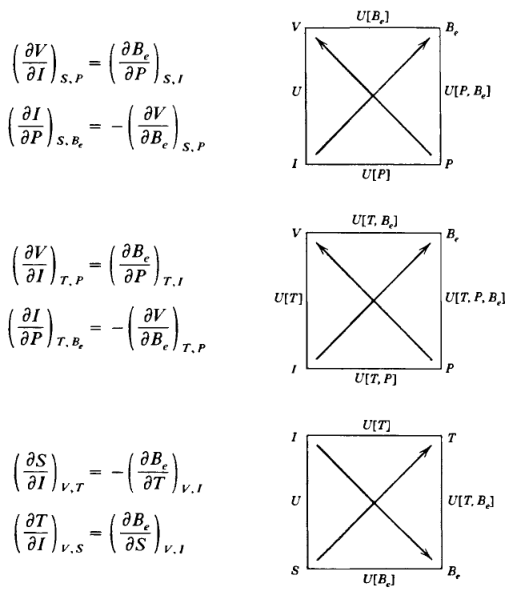
\includegraphics[width=\textwidth]{fig7_3.png}
	\figcaption{}
	\label{fig7.3}
}

“磁焓”$U[P, B_e] \equiv U + PV - B_e I$是有趣又有用的势函数。在压强、外磁场恒定的条件下,系统的磁焓取最小值。此外,根据\eqref{equ6.29}式的磁焓变体,$\rd U[P, B_e] = T\rd S = \dbar Q$($P, B_e, N$不变)。由此可见磁焓$U[P, B_e]$在压强、外磁场恒定的情况下就像系统的“热量势(potential for heat)”那样。

\begin{example}
某系统的基本方程与“顺磁模型”相同(\eqref{equ3.66}式),$T_0 = \SI{200}{K}, I_0^2 / 2R = \SI{10}{Tesla^2.K\per m^2.J}$。系统的摩尔数为$2$,在$B_e = \SI{0.2}{Tesla}$($\SI{2000}{gauss}$)的外磁场下保持压强恒定,从初始温度$\SI{5}{K}$加热到$\SI{10}{K}$. 求传入系统的能量。

{\bf 求解:}\\
传入系统的能量正是“磁焓”$U[P, B_e]$的改变量。顺磁模型的基本方程与体积无关,$P \equiv \partial U / \partial V = 0$, 于是$U[P, B_e]$退化到$U - B_e I = U[B_e]$. 再根据\eqref{equ3.66}式,$U = NRT, I = (NI_0^2 / 2RT) B_e$, 于是$U[P, B_e] = U[B_e] = NRT - (NI_0^2 / 2RT) B_e^2$. 因此 
\begin{align*}
	Q &= N \left[ R\Delta T - \frac{I_0^2}{2R} B_e^2 \Delta \left( \frac{1}{T} \right) \right] \\
	&= 2 [8314 \times 5 + 10 \times 0.04 \times 0.1] \,\mathrm{J} = \SI{83.15}{J}
\end{align*}

注意第二项的磁过程对传热的贡献相对于非磁过程(第一项)来说很小;实际中非磁过程对固体热容的贡献在低温下急剧降低,以至于比磁部分小。不妨回顾习题3.9-6.

\end{example}


\subsection*{习题}

%----------------------------------------------------------------------------------------
%	翻译:
%   校对:未校对!
%----------------------------------------------------------------------------------------


\chapter{热力学系统的稳定性}
\label{chap8}
\section{热力学系统的内在稳定性}
\label{sec3.1}
热力学中最基本的极值原理指出:$\text{d}S=0; \text{d}^2S<0$,第一个式子表示系统的熵取极值,第二个表明这个极值是极大值. 第二个式子决定着系统的稳定性,然而之前我们还没有完整地考察过这个式子. 与此相似,在力学中,一个单摆的稳定位置是其势能最小的位置. 而所谓处在“不稳定平衡”的位置与此相反,它正好在势能最大的地方.

对稳定性的考量将催生一些热力学中即有趣又重要的结论. 在本章中所考虑的条件都是可使系统达到稳定的条件. 在第9章中我们会考查相变(这是不稳定性的结果).

现在考虑两个完全相同的子系统,它们的基本方程都是$S=S(U,V,N)$,这两个子系统由完全不透的隔板分开. 我们假设$S$对$U$的依赖关系如图8.1\mpar{缺图}所示(定性地). 现在我们从第一个子系统中挪出$\Delta U$的能量到第二个烯勇中去,这时,总系统(由这两个子系统所组成)的熵就会由$2S(U,V,N)$变为$S(U+\Delta U,V,N)+S(U-\Delta U,V,N)$. 由图中可看出,总系统的熵竟然增大了\mpar{这是因为图中这个曲线的形状比较特别}. 显然,如果绝热限制被移除,那么能量就会自发地从一子系统流向另一个子系统,因之其中一个的能量会增多(温度也增加),另一个的能量减少. 这种情况甚至可以发生在一个子系统内,即能量从一个区域自发地转移到另一个区域,由此导致系统不均匀. 这种不均匀就是相变的特征.

从图8.1中我们可以看出,系统稳定的条件就是熵曲线上凹\mpar{这个图曲线下凹,所以会导致上面所说的熵增大的结果}.\footnote{R. B. Griffiths, \textit{J. Math. Phys.} \textbf{5}, 1215 (1964). L. Galgani and A. Scotti, \textit{Physica} \textbf{40}, (1968);\textbf{42},242(1969); \textit{Pure and Appl Chem.} \textbf{22}, 229(1970).}

\begin{equation}
\label{equ8.1}
S(U+\Delta U,V,N)+S(U-\Delta U,V,N)\leq 2S(U,V,N) \text{(for all $\Delta$)}
\end{equation}

如果$\Delta U\to 0$,那么该条件就变为微分式
\begin{equation}
\label{equ8.2}
\left(\frac{\partial^2S}{\partial U^2}\right)_{V,N}\leq 0
\end{equation}
但是这个微分式没上凹条件\ref{equ8.1}那么严格
,上凹条件需对所有的$\Delta U$成立,而非仅仅在$\Delta\to 0$时成立.

上面我们考虑的是能量的变化,如果我们考察体积的变化,结果是一样的
\begin{equation}
\label{equ8.3}
S(U,V+\Delta V,N)+S(U,V-\Delta V,N)\leq 2S(U,V,N)
\end{equation}
或写成微分形式
\begin{equation}
\label{equ8.4}
\left(\frac{\partial^2S}{\partial V^2}\right)_{U,N}\leq 0
\end{equation}

在由统计力学计算所得和试验测得的基本方程中,有一些确实不满足上凹条件.这时如果非要得到一个稳定的基本方程的话,我们可以按照图8.2所示的方法构造. 在真实的基本方程曲线上作切线,取那些处在曲线上方的切线,\textsf{稳定的状态方程就是这些取出来的切线的包络线}.

图8.2中,BCDEF线是不稳定的,这一可用直线BHF来代替. 实际上,真实的状态方程中,只有CDE段不满足微分形式的稳定性条件(也就是说局部不满足上凹条件). 因此整个曲线就不满足“全局”性的上凹条件\ref{equ8.1}.所以我们说该曲线中的BC和EF部分都是局域稳定但全局不稳定的.

直线(图8.2中的BHF)对应着两个相的分离,即系统中的一部分处于B状态,而另一部分处于F状态,我们将在第9章中详细解释这个问题.

在$S-U-V$组成的三维空间中,全局稳定要求熵曲面处于它的所有切面之下. 也就是说
\begin{equation}
\label{equ8.5}
S(U+\Delta U,V+\Delta V,N)+S(U-\Delta U,V-\Delta V,N)\leq 2S(U,V,N)
\end{equation}
由该式可推得\ref{equ8.2}\ref{equ8.4}和(参见问题8.1-1)
\begin{equation}
\label{equ8.6}
\frac{\partial^2S}{\partial U^2}\frac{\partial^2S}{\partial V^2}-\left(\frac{\partial^2S}{\partial U\partial V}\right)^\ge 0
\end{equation}
我们待会儿会通过另一种方法得到这个等式,该方法中我们会将一个类似\ref{equ8.2}的简单的曲率条件代入熵的Legendre变换中.

再次强调,全局稳定要求熵曲面处于它的所有切面之下. 相较之下,局部稳定要求的条件就弱一些,它只要求$\frac{\partial^2S}{\partial U^2}_{V,N}$和$\frac{\partial^2S}{\partial V^2}_{U,N}$都是负的且$\frac{\partial^2S}{\partial U^2}\frac{\partial^2S}{\partial V^2}-\left(\frac{\partial^2S}{\partial U\partial V}\right)^3$是正的.
$\frac{\partial^2S}{\partial U^2}<0$保证了:体积为常数的平面与S-U-V曲面的交线曲率为负(线上每一处都是平衡点).同样,$\frac{\partial^2S}{\partial V^2}<0$保证了:能量为常数的平面与S-U-V曲面形成的交线曲率为负.
这两个“偏曲率(partial curvatures)”并不能保证曲面上凹,因为曲面上可能这样一种凹槽,它在$\pm U, \pm V$四个方向上曲率为负,但在四个对角方向($U,V$坐标轴之间的对角线)上曲率为正. 第三个微分关系\ref{equ8.6}正是限制了这种情况的发生.

以物理的语言来说,局域稳定条件保证了系统中各部分的$u\text{或}v$之间的不均匀不会导致熵增加,也保证了$u,v$共同的不均匀行为不会导致熵增加.

对于磁体系而言也有类似的关系,只不过磁矩代替了体积的角色.

在彻底阐明这些稳定条件之前,我们先来考察一下其他类似的关系(不同的热力学势有不同的关系).我们先看一个意义最明显的关系(\ref{equ8.3}),搞清楚它蕴含的信息,其他的关系也包含着类似的东西. 方程\ref{equ8.2}要求
\begin{equation}
\label{equ8.7}
\left(\frac{\partial^2S}{\partial U^2}\right)_{V,N}=-\frac{1}{T^2}\left(\frac{\partial T}{\partial U}_{V,N}=-\frac{1}{NT^2c_v}\leq 0\right)
\end{equation} 
因此,一个稳定系统的摩尔热容必须为正. 类似地。其他稳定性条件也会对一些可观测物理量作出限制.

最后我们做个总结,在一个$r+2$维的热力学空间$(S,X_0,X_1,\cdots,X_r)$中,系统的稳定性要求
熵曲面处于它的所有切面之下.





\section{其他热力学势的稳定性条件}
\label{sec3.2}
如果要在能量表象下重新表述稳定性准则,我们只需要简单作一个转述就行. 既然要求熵最大能量最小,那么熵曲面的上凹性就可以转化为能量曲面的下凹性.

稳定能量曲面总处于它的切面之上.
\begin{equation}
\label{equ8.8}
U(S+\Delta S,V+\Delta V,N)+U(S-\Delta S,V-\Delta V,N)\geq 2U(S,V,N)
\end{equation}

局域下凹条件变为
\begin{equation}
\label{equ8.9}
\frac{\partial^2U}{\partial S^2}=\frac{\partial T}{\partial S}\geq 0\qquad \frac{\partial^2U}{\partial V^2}=-\frac{\partial P}{\partial V}\geq 0
\end{equation}

附加$S,V$一同变化时的限制条件
\begin{equation}
\label{equ8.10}
\frac{\partial^2U}{\partial S^2}\frac{\partial^2U}{\partial V^2}-\left(\frac{\partial^2U}{\partial S\partial V}\right)^2\geq 0
\end{equation}

更严格一些的做法是:对能量或熵进行Legendre变换. 首先复习一些勒让德变换得性质(见式\ref{equ5.31})
\begin{equation}
\label{equ8.11}
P=-\frac{\partial U}{\partial X}\qquad\text{及}\qquad X=-\frac{U[P]}{\partial P}
\end{equation}

因之

\begin{equation}
\label{equ8.12}
\frac{\partial X}{\partial P}=-\frac{\partial^2U[P]}{\partial P^2}=\dfrac{1}{\frac{\partial^2U}{\partial X^2}}
\end{equation}

所以$\partial^2U[P]/\partial P^2$与$\partial^2U/\partial X^2$的符号相反.那么,如果$U$是$X$的一个上凹函数,则$U[P]$是一个关于$P$的下凹函数. 用同样得方式可知,Helmholtz势是温度的上凹函数,是体积的下凹函数.
\begin{equation}
\label{equ8.13}
\left(\frac{\partial^2 F}{\partial T^2}\right)_{V,N}\leq 0\qquad \left(\frac{\partial^2 F}{\partial V^2}\right)_{T,N}\geq 0
\end{equation}

焓是熵的上凹函数,压强的下凹函数
\begin{equation}
\label{equ8.14}
\left(\frac{\partial^2 H}{\partial S^2}\right)_{P,N}\geq 0\qquad \left(\frac{\partial^2 H}{\partial P^2}\right)_{S,N}\leq 0
\end{equation}
吉布斯势既是温度也是压强的下凹函数
\begin{equation}
\label{equ8.15}
\left(\frac{\partial^2 G}{\partial T^2}\right)_{P,N}\leq 0\qquad \left(\frac{\partial^2 G}{\partial P^2}\right)_{T,N}\leq 0
\end{equation}

总结起来,$N$恒定时,对各个热力学势的特征变量而言,对应热力学势($U$及其Legendre变换)是强度量的下凹函数,广延量的上凹函数. 同样地,$N$恒定时Massieu函数(熵及其Legendre变换)是对应强度量的上凹函数,广延量的下凹函数.

\section{热力学系统的内在稳定性}
\label{sec8.3}
由稳定性准则能导出哪些物理结论?本节将讨论这个问题.稳定性准则将限制诸如$c_v, c_p,\alpha,\kappa_T$这些量的正负.第一个推论为:$c_v>0$,可由\ref{equ8.2}或\ref{equ8.7}导出. 类似地,由Helmholtz势关于体积$V$的上凹性将得到
\begin{equation}
\label{equ8.16}
\left(\frac{\partial^2F}{\partial V^2}\right)_T=-\left(\frac{\partial P}{\partial V}\right)_T=\frac{1}{V_{\kappa_T}}\ge 0
\end{equation}
或
\begin{equation}
\label{equ8.17}
\kappa_T\ge 0
\end{equation}

由$c_v, \kappa_T$还能获得更多的信息。如果回想一下在\textsl{问题3.9-5}中所得的等式
\begin{equation}
\label{equ8.18}
c_p-c_v=\frac{Tv\alpha^2}{\kappa_T}
\end{equation}
和
\begin{equation}
\frac{\kappa_s}{\kappa_T}=\frac{c_v}{c_P}
\end{equation}
结合之前稳定性准则导出的结论,我们马上就能知道
\begin{equation}
c_p\ge c_v\ge 0
\end{equation}
和
\begin{equation}
\kappa_T\ge\kappa_s\ge 0
\end{equation}

因此在一个稳定系统中,热容和压缩率一定是正的. 即:\textsl{向满足稳定性准则的系统中加入热量,无论于恒压或恒容条件下,都将增加系统的温度——且恒容时比恒压时增加得更多.减少系统的体积,无论于绝热或恒温条件下,都将增大系统的压强——且绝热时比恒温时增加得更多}

\section{Le Chatelier 原理;涨落的定性影响}
\label{sec8.4}
稳定性准则的物理内涵就是著名的\textsl{Le Chatelier 原理}. 据该原理,稳定性可描述为:\textsl{系统中发生的会产生不均一性的事件的都会诱发一个趋向于抵消该事件的过程.}

举个例子,考虑一容器中处于平衡的液体,某时刻一光子射入液体,它将液体局部稍稍加热了一点. 根据稳定性条件,热量会从被加热的区域流走,被加热区域的温度因此而向周围环境的温度靠近,系统重建了平衡.

与此相类,液体中传播的纵波会让系统中一些地方的密度或高或低. 如果某区域密度增高,那么压强也随之增高,因而该处的液体趋向于散开,反之密度低的区域将趋向于收缩.稳定性条件(即压缩率为正)确保了这些响应将使系统重建平衡.

实际上,局域的不均一经常出现在物理系统中,除入射光和外界引起的振动外,还有很多其他诱因. 比如气体中,每个分子都在随机运动,运气好的话,就会产生密度高一些和低一些的区域.

若以统计力学观点视之,则所有系统都会有永不停歇的局部涨落. 经典热力学认为平衡态就是静止的、但实际上平衡是动态的. 局域的不均一无时无刻不在发生,只是\textsl{Le Chatelier 原理}让我们以为只有外部扰动才会产生不均一罢了.

热力学系统与一个在拱墙上滚动的鹅卵石很像. 石头的稳定点就在拱墙势能的最小点. 稳定性准则则要求墙面是上凹的.

如果考虑得更巧妙些,我们可将石头视作服从Brownian运动——石头可能会经历各种各样的随机碰撞. 这个力学上的例子与真实系统中的自发涨落很相像. 势能最小点并非对应系统中的一个瞬时点,而是一期望值,这种期望值其实就是热力学所描述的东西. 拱墙的曲率有着持续的、决定性的作用,它使系统在每次Brownian碰撞(涨落)后都回归到"期望态"中.

需要指出,如果鹅卵石在一个既浅又不对称的拱壁内运动,则鹅卵石的“期望态(能量最低点)”可能会与平均位置(时间平均)不太一样. 在这种情况下,经典热力学的预测与实际观测不符,实际观测得到的是时间平均值(回顾第一章). 这种异常状态会发生于高阶相变中——实际上直到1970年代,正确的理论才发展出来. 到第11章我们再来探索这个问题.

\section{Le Chatelier-Braun原理}
\label{sec8.5}
回到稳定性准则的物理诠释. \textsl{Le Chatelier 原理}给出了一种诠释,然而更有洞见的则是\textsl{Le Chatelier-Braun原理}.
假设某一系统由于某些作用或者涨落而偏离了平衡态. 根据\textsl{Le Chatelier 原理},这个微扰会诱发一个削弱微扰本身的过程. 然而随之发生的还有一些二级过程. \textsl{Le Chatelier-Braun原理}说:这些非直接引发的二级过程同样会削弱最初的扰动.

我们来看一个简单的例子.一活塞筒的壁透热,将其置于“浴”中(放在一个既是热库又是压力库的库中),活塞是松弛的\mpar{松弛的意思是:活塞刚好能塞住圆筒内的气体,如果装的是气体的话.}.由于存在涨落或者可能的外力,活塞向外缓慢移动. 最直接的影响就是系统内的压强下降——这就造成了内外压强差并导致活塞被压回,这是\textsl{Le Chatelier 原理}的结果. 现在来考虑二级效应,活塞向外移动,系统体积增加$\text{d}V$,体积的变化导致温度的变化:$\text{d}T=(\partial T/\partial V)_S\text{d}V=-(T_\alpha/Nc_v\kappa_T)\text{d}V$\mpar{为什么是绝热?因为此时作者考虑的是一个瞬时的过程,如果系统的透热壁传热速度不是无穷大,那么在dT内发生的体积变化就是一绝热过程.},温度改变量的正负取决于$\alpha$. 由于产生了温度差,所有会有热量流过圆筒壁,如果$\alpha$为正,则热量流入,反之则流出(\text{sign} $\dbar Q$=\text{sign} $\alpha$). 热流反过来又会改变系统的压强:$\text{d}P=(1/T)(\partial P/\partial S)_V\dbar Q=(\alpha/NT^2c_v\kappa_T)\dbar Q$.  无论$\alpha$正负,压强都将增加. 因此,这个诱导出的二级过程(热流)也将最初的微扰削弱了. 此之谓\textsl{Le Chatelier-Braun原理}.

为严格证明\textsl{Le Chatelier 原理}和\textsl{Le Chatelier-Braun原理},设想一个复合系统中的自发涨落$\text{d}X^f_1 $. 随变量$X$涨落而发生的还有子系统中对应强度量$P_1$的改变:
\begin{equation}
\label{equ8.22}
\text{d}P_1^f= \frac{\partial P_1}{\partial X_1}\text{d}X_1^f 
\end{equation}
涨落$\text{d}X_1^f $可能也会改变强度量$P_2$
\begin{equation}
\label{equ8.23}
\text{d}P_2^f= \frac{\partial P_2}{\partial X_1}\text{d}X_1^f 
\end{equation}
现在来考察强度量$\text{d}P_1^f, \text{d}P_2^f$会反过来对$X_1, X_2$产生何影响. 我们将这种反馈改变量$\text{d}X_f $记作$\text{d}X_f^r$,上标\text{r}代表英文response. $\text{d}X_1^r, \text{d}X_2^r$的符号可以通过求总能的最小值来得到(此时总熵恒定)
\begin{eqnarray}
\label{equ8.24}
\text{d}(U+U^\text{res})&=(P_1-P_1^\text{res})\text{d}X_1^r+(P_2-P_2^\text{res}){d}X_2^r\leq 0\\
&=\text{d}P_1^f\text{d}X_1^r+\text{d}P_2^f\text{d}X_2^r\leq 0
\end{eqnarray}
因之,再考虑到$\text{d}X_1^r, \text{d}X_1^r$是独立的,就有
\begin{equation}
\label{equ8.26}
\text{d}P_1^f\text{d}X_1^r\leq 0
\end{equation}
和
\begin{equation}
\label{equ8.27}
\text{d}P_2^f\text{d}X_2^r\leq 0
\end{equation}
从\ref{equ8.26}和\ref{equ8.22}可知
\begin{equation}
\label{equ8.28}
\frac{\text{d}P_1}{\text{d}X_1}\text{d}X_1^f\text{d}X_1^r\le 0
\end{equation}
同理可得
\begin{equation}
\label{equ8.29}
\frac{\text{d}P_2}{\text{d}X_1}\text{d}X_1^f\text{d}X_2^r\le 0
\end{equation}\mpar{原文该式为$\frac{\text{d}P_2}{\text{d}X_1}\text{d}X_1^f\text{d}X_2^f\le 0$,是一处显然的笔误,现改正}

现在来考察这两个结果. 第一个是\ref{equ8.28},此即\textsl{Le Chatelier 原理}的数学表达式. 将该式乘以$\text{d}P_1/\text{d}X_1 $,根据稳定性的上凹性准则,可知$\text{d}P_1/\text{d}X_1$为正,所以
\begin{equation}
\label{equ8.30}
\frac{\text{d}P_1}{\text{d}X_1} \text{d}X_1^f\cdot \frac{\text{d}P_1}{\text{d}X_1} \text{d}X_1^r \le 0
\end{equation}
或
\begin{equation}
\label{equ8.31}
{\text{d}P_1^f}{\text{d}P_1^{r(1)}} \le 0
\end{equation}
也就是说,初始扰动引发了$P_1$的变动$\text{d}{P_1^f}$,该变动反馈给$X_1$,产生了$X_1$的反馈变动$\text{d}X_1^r$,该反馈变动又诱发了$P_1$的变动$\text{d}P_1^{r(1)} $,$\text{d}P_1^{r(1)} $恰好与$\text{d}{P_1^f}$反号.

第二个不等式\ref{equ8.29},借助Maxwell关系
\begin{equation}
\label{equ8.32}
\frac{\partial P_2}{\partial X_1}=\frac{\partial P_1}{\partial X_2}
\end{equation}
可以重新表述为
\begin{equation}
\label{equ8.33}
\text{d}X_1^f\cdot\left(\frac{\partial P_1}{\partial X_2}\text{d}X_1^r \right)\leq 0 
\end{equation}
然后用$\text{d}P_1 /\text{d}X_1$(其值是正的)乘上式得
\begin{equation}
\label{8.34}
\left(\frac{\partial P_1}{\partial X_1}\text{d}X_1^f\right)\cdot \left(\frac{\partial P_1}{\partial X_2}\text{d}X_1^r\right)\leq 0
\end{equation}
或
\begin{equation}
\label{8.35}
(\text{d}P_1^f )(\text{d}P_1^{r(2)} )\leq 0
\end{equation}

也就是说,反馈响应$\text{d}X_2^r$诱发了$P_1$的改变量$\text{d}_1^{r(2)} $,它与初始扰动引发的改变$\text{d}P_1 $反号.此之谓\textsl{Le Chatelier-Braun原理}

最后要指出,方程\ref{equ8.33}也有一个有趣的解释. 用$\text{d}P_2/\text{d}X_2$(其值为正)乘\ref{equ8.33}得
\begin{equation}
\label{equ8.36}
\left(\frac{\partial P_2}{\partial X_1}\text{d}X_1^f\right)\cdot \left(\frac{\partial P_2}{\partial X_2^r}\text{d}X_2^r\right)\leq 0
\end{equation}
或
\begin{equation}
(\text{d}P_2^f )(\text{d}P_2^{r(2)} )\leq 0
\end{equation}
这就是说,$X_2$的响应诱发了$P_2$的改变,且这个改变与关于$X_1$的初始扰动所诱发的$P_2$的改变量反号.

%!TEX root = ../CallenThermo.tex
% - 翻译:CuI
\chapter{一级相变}
\label{chap9}

\section{能量最小原理}
\label{sec9.1}

通常情况下在室温和大气压的条件下水是液体,
但是如果被冷却到$273.15K$以下就会凝固;
而如果被加热到$373.15K$以上就会汽化。
在这些温度下物质的性质都会发生急剧的变化——也就是“相变”。
在高压下水会经历一些额外的从一种固态到另一种固态的相变过程。
这些不同的固相,被定为“冰I”,“冰II”,“冰III”,……,在晶体结构以及基本所有热力学性质上都不同(比如压缩系数,摩尔热容,以及各种摩尔势比如$u$或者$f$)。
水的“相图”如图\ref{fig9.1}所示。

每一个相变都对应着热力学基本关系的一个线性区域(比如图\ref{fig8.2}的$BHF$),
并且每一个都可以看成潜在的基本关系中稳定条件(凸的或者凹的)失效的结果。

在本节中我们要考虑基本关系不稳定的系统。
通过定性考虑这种系统的涨落我们会看到{\it 涨落会受到潜在的基本关系的细节的深刻影响}。
与此相对的,{\it 广延量的均值只能反应稳定的热力学基本关系。}

关于潜在的基本关系的形式对于热力学涨落的影响方式的考虑会给
第\ref{chap8}章中稳定性的考虑以及图\ref{fig8.2}的构造(其中热力学基本关系是通过切平面的包络构造出来的)提供物理解释。

一个简单的力学模型可以通过一个直观易懂的类比来解释这种考虑。
考虑一段半圆形的两端封闭的管子。
这个管子如同倒着的$U$型垂直竖立在桌子上(图\ref{fig9.2})。
这个管子内包含一个可以自由移动的活塞将其分成两部分,
每一部分都包含一摩尔的气体。
这个系统的对称性会被证明有重要的效果,
而为了破坏这个对称性我们考虑管子的每一段含有一个小的金属“滚珠”(也就是一个小的金属球)。
两个金属球是热膨胀系数不同的两种金属构成的。

在一些特别的温度下,比如我们记为$T_c$,两个金属球的半径相同;
而在温度高于$T_c$的时候,右边的球更大。

活塞暂时被放在管子的顶端,可以落入两条腿中的任意一个,
从而压缩那一条腿中的气体,而另一条腿中的气体则会膨胀。
在这两种互斥的平衡态中,压强差都正好被活塞质量的效果补偿。

如果没有这两个滚珠的话这两个互斥的平衡态是完全等价的。
但当存在滚珠的时候,如果$T>T_c$那么落入左边是一个更加稳定的平衡态,
如果$T<T_c$那么落入右边就成了更加稳定的平衡态。

从热力学的观点来看,系统的 Helmholtz 势是$F=U-TS$,
而能量$U$包含了活塞的重力势能以及我们所熟悉的两部分气体的热力学能量
(当然也包括两个滚珠的内能,不过我们假定这部分很小而且两者相同)。
从而系统的Helmholtz势就有两个局域极小值,
而更低的哪一个极小值对应着活塞落入包含的球更下的那一侧。

活塞从一边到另一边的平衡位置之间的移动也可以通过在给定温度下倾斜桌子达到类似的效果——或者在类似的热力学中,通过加入一些温度以外的热力学参数实现。

平衡态从一个局域极小移动到另一个构成了{\it 一级相变},
这是由于温度或者其它热力学参数的改变导致的。

{\it 一级相变联系的两个态是有区别的,它们出现在热力学构型空间中独立的区域。}

为了讨论“临界现象”和“二级相变”(第\ref{chap10}章),
暂时考虑滚珠全同或者不存在的情况会很有用。
于是在低温时两个互斥的极小值是等价的。
不过随着温度的升高,活塞的两个平衡位置会在管子中上升接近顶端。
超过一个特别的温度$T_{cr}$以后,就只有活塞位于管子的顶端这一个平衡位置了。
相反地,如果把温度从$T>T_{cr}$降到$T<T_{cr}$,
这唯一的平衡态会分成两个(对称的)平衡态。
这个温度$T_{cr}$就是“临界温度”而在$T_{cr}$的变化就是“二级相变”。

{\it 二级相变联系的两个态在热力学构型空间中是连续的。}

在这一章中我们考虑一级相变。
二级相变会在第\ref{chap10}章中讨论。
在那里我们也会对这个“力学模型”做定量地考虑,尽管在这里我们仅仅做了定性的讨论。

回到两个球不同的情况,考虑活塞位于更大的极小值——
也就是跟更大的滚珠位于管子的同一侧。
处于Helmholtz势那样的一个极小值时,
即使经历热涨落(“布朗运动”)活塞也会暂时保持在那个极小值处。
在足够场的时间后一个巨大的涨落会带动活塞“越过顶端”并达到稳定的极小值。
之后它就会呆在这个更深的极小值处知道一个更大(也更加不可能)的扰动把它待会次稳定的极小值处,然后这整个过程会反复重现。
随着幅度的增大涨落的概率会下降得非常快(我们会在第\ref{chap19}章看到这一点)
以至于{\it 在大部分时间中系统会位于更加稳定的极小值处。}
宏观热力学中多有这些动力学都被忽略了,因为它只关心稳定的平衡态。

为了在更加偏向热力学的环境中讨论相变的动力学,
把我们的注意力转移到更加熟悉的热力学系统会更加方便,
它的热力学势同样具有两个局域极小值并且被一段凹的不稳定区域分开。
特别地我们考虑一个容器中压力为一个大气压而且温度高于$373.15K$的水蒸气(也就是高于水的“常规沸点”)。
我们把注意力集中到一个小的子系统——一个半径大小(可以改变)使得任意时刻都包含有一毫克水的球形区域。
这个子系统等价于跟一个热库和一个蓄压器接触,
而平衡条件是子系统的Gibbs势$G(T,P,N)$处于极小值。
由平衡条件决定的两个独立变量是子系统的能量$U$和体积$V$。

如果Gibbs势形如图\ref{fig9.3}所示那样,
其中$X_j$是体积,那么系统在更低的极小值处是稳定的。
这个极小值对应着比第二局域极小值更大的体积(或者更小的密度)。

考虑体积涨落的行为。
这种涨落是自发而且连续发生的。
图\ref{fig9.3}中曲线的斜率表征了一个强度量(在当前情况下与压强不同),
它扮演着符合Le Chatelier 原理使系统密度趋于均匀的回复“力”的角色。
偶尔涨落会太大以至于使得系统越过极大值,达到第二个极大值的区域。
接下来系统就会呆在第二个极小值区域——不过只会呆一小会儿。
要跨过第二个极小值处更低的势垒,一个更小(因此也就更加常见)的涨落就足够了。
系统很快就回到了它的稳定态。
因此很小的高密度液滴(液相!)偶尔会在气体中形成,存在一小会儿然后消失。

如果第二个极小值距离最小值很远,而且它们之间的势垒很高,
那么从一个到另一个的涨落就会变得非常不可能。
在第\ref{chap19}章中会说明,这类涨落的概率会随着中间自由能的势垒的高度指数下降。
在固态系统(其中相互作用能量比较高)中由于中间势垒高得让从一个极小值变到另一个的时间的量级超过了宇宙的年龄,所以通常不会有多个极小值。
陷入这种“亚稳态”极小值的系统{\it 实际上}处于稳定平衡态(就像更深的极小值并不存在一样)。

回到水蒸气处于高于“沸点”的某个温度的情形,假设我们降低整个系统的温度。
Gibbs势的变化形式如同图\ref{fig9.4}中显示的那样。
在温度$T_4$两个极小值会相等,而在这个温度以下,高密度(液体)相会变成绝对稳定的。
因此$T_4$就是相变的温度(在给定的压力下)。

如果蒸汽从相变温度缓慢冷却,系统会发现之前所处的绝对稳态现在变成了亚稳态。
迟早系统的一个涨落就会“发现”真正的稳态,形成液体凝结核。
这个核会迅速变大,然后整个系统会突然经历相变。
实际上系统通过一个“试探”涨落发现更稳定的态所需的时间在蒸汽到液体凝结的情况下短到难以观察。
不过在从液体到冰的持续时间在一个纯粹的情况下很容易观察到。
被冷却到低于凝固点(结冰)温度的液体被称为是“过冷的”。
轻轻敲一下容器,产生的纵波就会导致多个“密集”和“稀疏”的区域,
而这些外部诱导的涨落会代替自发的涨落引发剧烈的相变。

当把Gibbs势的极小处的值相对温度画出来的时候会引出一个有用的视角。
这个结果如图\ref{fig9.5}所示。
如果从图\ref{fig9.4}中选取极小值那么久会只有两个这种曲线,
不过任意数值都是可能的。
在平衡态最小的极小值是稳定的,所以真正的Gibbs势是图\ref{fig9.5}中的曲线的下包络。
熵的不连续(也就是潜热)对应着包络函数斜率的不连续。

图\ref{fig9.5}需要增加一个额外的维度,增加的坐标$P$作用类似于$T$。
于是Gibbs势就被表示成下包络曲面,和三个单个的相面重合。
这些曲面之间相交曲线在$P-T$平面上的投影就是我们熟悉的相图(比如图\ref{fig9.1})。

相变发生在系统从一个包络曲面越过相交线到另一个包络曲面时所处的态。

图\ref{fig9.4}的变量$X_j$或者$V$可以是任意广延量。
在顺磁到铁磁的相变中,$X_j$是磁矩。
在从一种晶体形式到另一种晶体形式的相变中(比如从立方体到六边形)
相应的参数$X_j$是一个晶体对称性变量。
在溶解度的相变中则可能是一种组分的摩尔数。
随后我们会看到这类相变的例子。
这些都符合前面描述的一般模式。

在一级相变中两个相的摩尔Gibbs势是相等的,但是其它摩尔势(比如$u,t,f$)
在相变前后是不连续的,摩尔体积和摩尔熵也是如此。
两种相占据了“热力学空间”的不同区域,而除了Gibbs势以外任何性质的相等都只是巧合。
摩尔势的不连续性就是定义一级相变的性质。

如图\ref{fig9.6}所示,如果沿气液共存曲线远离固相(也就是向着更高的温度),
摩尔体积和摩尔能量的间断会逐渐变小。
两种相会变得越来越相似。
最再气液共存曲线的终点,两种相会变得不可分辨。
一级相变会退化成一个更加微妙的相变,也就是我们将会在第\ref{chap10}章中介绍的{\it 二级相变}。
共存曲线的终点被称为{\it 临界点}。

临界点的存在阻碍了我们明确区分通称为{\it 气体}和通称为{\it 液体}的可能性。
在通过一级相变穿过气液共存曲线的时候,我们区分了两种态,
一个“明确”为气体而另一个“明确”为液体。
但从其中一个开始(比如液体,处于共存曲线上方)
我们可以沿着任意一条绕过临界点的路径到达另一个态(“气”态)而不经历相变!
从而通称的{\it 气体}和{\it 液体}相较于严格定义的记法更多是直觉上的含义。
液体和气体共同组成了{\it 流体相}。
除此以外我们在气液一级相变中对于“液相”和“气相”应该遵循标准的用法。

在图\ref{fig9.1}中有另一个非常有趣的点:气液共存曲线的另一个终点。
这个点是三条共存曲线的交点,它也是唯一一个气相液相和固相共存的点。
这种三相相容的点被称为“三相点”——这里是水的三相点。
被唯一确定的水的三相点的温度被定义(可以是任意的)为
Kelvin温标下的$273.16K$这一数值(在第\ref{sec2.6}节中已经介绍过)。

\section{熵的不连续——潜热}
\label{sec9.2}

类似图\ref{fig9.1}的相图被共存曲线分为不同的使得某一种相是稳定态的区域。
这些曲线上的每一点两种相都具有完全一样的摩尔Gibbs势,因此两种相可以共存。
考虑水处于图\ref{fig9.1}a中“冰”这一区域的某个温度和压强下。
为了增加冰的温度,每使温度升高一Kelvin我们都要提供大概$2.1kJ/kg$的热量
(冰的比热容)。
如果用固定的速度提供热量,温度也会以几乎固定的速度增加。
但当温度到达气液共存线上的"熔化温度",温度就不再增加了。
如果继续供热,冰就会熔化形成同样温度的水。
熔化每$kg$的冰需要$335kJ$的热量。
在系统到达共存曲线后(也就是处于熔点温度),
任意时刻容器中水的多少都决定于进入容器的热量的多少。
当最终供给足够多的热量的时候,冰会完全熔化,继续加热会再次导致温度的升高——
而此时的速率是由水的比热容决定的($\simeq 4.2kJ/kg-K$).

一摩尔固体熔化需要的热量就是{\it 融化热}(或者叫{\it 熔化潜热})。
它和气相与固相的摩尔熵的差相联系。
\begin{equation}
\label{equ9.1}
\ell_{LS}=T[s^{(L)}-s^{(S)}]
\end{equation}
其中$T$是给定压强下熔点的温度。

更一般地,任何一级相变的潜热是
\begin{equation}
\label{equ9.2}
\ell=T\Delta s
\end{equation}
其中$T$是相变发生的温度而$\Delta s$是两种相的摩尔熵的差。
或者潜热可以写成两种相摩尔焓的差
\begin{equation}
\label{equ9.3}
\ell=\Delta h
\end{equation}
这可以直接从恒等式$h=Ts+\mu$
(以及摩尔Gibbs函数$\mu$在两种相中都相等这一事实)中得出。
对于很多情况每一种相的摩尔焓都被做成了表。

如果相变发生在气相和液相之间,潜热被称为{\it 汽化热},
而如果发生在气相和固相之间,则被称为{\it 升华热}。

在一个大气压下水的气液相变(沸腾)发生在$373.15K$,
而汽化潜热是$40.7kJ/mole$($540cal/g$)。

在每一种情况下系统从低温相变为高温相都需要{\it 吸收}相应的潜热。
高温相的摩尔熵和摩尔焓都比低温相的要高。

需要注意的是诱使相变发生的手段是不相干的——潜热与之无关。
除了在确定的压强下加热冰(“水平地”穿过图\ref{fig9.1}a中的共存曲线),
也可以在确定的温度下加压(“竖直地”穿过共存曲线)。
两种情况下从热库中提取的潜热是相同的。

实用的水气液共存曲线的形式由“饱和蒸汽表”给出——
名称中的“饱和”代表着蒸汽和液相处于平衡。
(“过热蒸汽表”只编写了蒸汽相的性质。)
来自于Sonntag 和Van Wylen的表9.1给出了这种饱和蒸汽表的一个例子。
每一种相的属性$s,u,v$和$h$都按照惯例列在这些表中;
每一种相变的潜热都是两种相的摩尔焓的差,或者也可以用$T\Delta s$得到。

在热物理数据手册中对于很多种其他的物质都按照这种方式给出了类似的数据。

摩尔体积和摩尔熵与摩尔能量一样,在越过共存曲线的时候是不连续的。
对于水的共存曲线来说这特别有趣。
通常的经验中冰会在液态水中漂浮。
从而固相(冰)的摩尔体积要比液相的摩尔体积{\it 更大}——
这是$H_2O$的一个不平常的特性。
更常见的情况是固相更加致密,拥有更下的摩尔体积。
$H_2O$这个特殊性质的一个平凡的后果就是冰冻水管会胀裂。
而我们在第\ref{sec9.3}中会看到作为一个补偿性的后果就是可以滑冰。
而全部后果中最根本的,是水的这个特殊性质是地球上可以存在生命所必需的。
如果并比液态水更加致密,寒冷的冬天湖和海洋的表面冻结后会沉底;
表面新的液体由于没有了冰层的保护,会继续冻结(并且下沉)
直到所有水都被冻成固态(“下面结冻”而不是“上面结冻”)。

\section{共存曲线的斜率;Clapeyron 方程}
\label{sec9.3}

图\ref{fig9.1}中所示共存曲线并不如直观看起来那么任意;
共存曲线的斜率$dP/dT$完全由两个共存相的性质决定。

共存曲线的斜率物理上是很有趣的。
考虑一个立方体的冰在一玻璃杯的水中处于平衡。
给定外界的压强,那么这个混合系统的温度就由水的固液共存曲线决定了;
如果温度并不在共存曲线上,那要么有些冰会熔化,要么有些水会凝固,
知道温度再次回到共存曲线上(或者其中一个相会消失)。
在一个大气压下,温度会是$273.15K$。
如果外界气压下降——可能由于高度改变导致(这杯水是由一架飞机上的空乘提供的),
或者由于大气条件的改变(风暴的接近)
——于是这杯水的温度会恰当地调整到共存曲线上一个新的点上。
如果压强的改变是$\Delta P$那么温度的改变就是
$\Delta T=\Delta P/(dP/dT)_{cc}$,
其中分母上的导数是共存曲线的斜率。

我们前面提及的滑冰提供了另一个有趣的例子。
冰刀对下面冰的压力会使得冰越过固液共存曲线(图\ref{fig9.2}中竖直向上),
在滑过的表面上共一个液体的润滑层。

滑冰之所可行是由于水的固液共存曲线斜率是负的。
冰会存在于湖的上表面而不是在底部,反应了水的固相的摩尔体积要比液相的大。
这两个并不互相独立的事实的关联,隐含在现在我们要关注的Clapeyron方程中。

考虑如图\ref{fig9.7}所示的四个态。
态$A$和$A'$在共存曲线上,但是他们对应着不同的相
(分别对应着左手边的区域和右手边的区域。)
态$B$和$B'$也类似。
压强差$P_B-P_A$(或者等价地,$P_{B'}-P_{A'}$)
被假设为是无穷小量($=dP$),而温度差$T_B-T_A$($=dP$)也类似。
曲线的斜率是$dP/dT$。

相平衡要求
\begin{equation}
\label{equ9.4}
\mu_A=\mu_{A'}
\end{equation}
以及
\begin{equation}
\label{equ9.5}
\mu_B=\mu_{B'}
\end{equation}
因此
\begin{equation}
\label{equ9.6}
\mu_B-\mu_A=\mu_{B'}-\mu_{A'}
\end{equation}
不过我们又有
\begin{equation}
\label{equ9.7}
\mu_B-\mu_A=-sdT+vdP
\end{equation}
和
\begin{equation}
\label{equ9.8}
\mu_{B'}-\mu_{A'}=-s'dT+v'dP
\end{equation}
其中$s$和$s'$是两个相的摩尔熵而$v$和$v'$是它们的摩尔体积。
通过把方程\eqref{equ9.7}和\eqref{equ9.8}代入方程\eqref{equ9.6}
并重新组合,我们很容易发现
\begin{equation}
\label{equ9.9}
\frac{dP}{dT}=\frac{s'-s}{v'-v}
\end{equation}
\begin{equation}
\label{equ9.10}
\frac{dP}{dT}=\frac{\Delta s}{\Delta v}
\end{equation}
其中$\Delta s$和$\Delta v$是相变对应的摩尔熵和摩尔体积的变化。
根据方程\eqref{equ9.2},潜热是
\begin{equation}
\label{equ9.11}
\ell=T\Delta s
\end{equation}
因此
\begin{equation}
\label{equ9.12}
\frac{dP}{dT}=\frac{\ell}{T\Delta v}
\end{equation}
这就是Clapeyron方程。

Clapeyron方程体现了Le Chatelier原理。
考虑固液相变中潜热为正($s_l>s_s$)并且摩尔体积变化为正($v_l>v_s$)的情况。
相曲线的斜率是正的。
于是固定温度下增加压强就会推动系统到一个更加致密(固体)的相(缓解压强增加),
而温度的增加会推动系统到一个熵更大(液体)的相。
相反地,如果$s_l>s_s$但是$v_l<v_s$,共存曲线的斜率就是负的,
因此增加压强(固定温度$T$下)就会推动系统变到液相——依然是一个更加致密的相。

在应用Clapeyron方程的实践问题中,相对气相忽略液相的摩尔体积
($v_g-v_l\simeq v_g$),并且用理想气体方程($vg\simeq RT/P$)
来近似气体的摩尔体积是可以的。
这个“Clapeyron-Clausius 近似”可以适用于这一节后面的问题。

{\bf 例题}

一个截面为矩形的刚体金属棒平放在一块冰上,两端都伸出一点。
棒的宽度是$2mm$,和冰接触的长度是$25cm$。
两个质量均为$M$的物体分别挂在棒的两端。
整个系统处于大气压强下,并且温度保持在$T=-2^\circ C$。
那么如果想要让金属棒通过熔化后再重新结冰的方式通过冰块,
所需要的$M$的最小值是多少?
给出的数据有水的凝固潜热是$80cal/g$,水的密度是$1g/cm^3$,
以及冰块浮在水面上的时候$\simeq 4/5$的体积淹没在水面下。

{\bf 解答}

Clapeyron方程允许我们找出在$T=-2^\circ C$的时候发生固液相变的压强。
不过我们必须首先用“冰立方数据”来得到固相和液相的摩尔体积差$\Delta v$。
数据给出冰的密度是$0.8g/cm^3$。
更进一步有$\nu_{liq}\simeq 18cm^3/mole$,
以及$\nu_{solid}\simeq 22.5 \times 10^{-6} m^3/mole$。
从而
\begin{equation*}
\left.\frac{dP}{dT}\right)_{cc}=\frac{\ell}{T\Delta v}
=\frac{80\times4.2\times18J/mole}{271\times(-4.5\times10^{-6}Km^3/mole}
=-5\times10^6Pa/K
\end{equation*}
所以需要的压强差就是
\begin{equation*}
P\simeq-5\times10^6\times(-2)\simeq10^7Pa
\end{equation*}
这个压强是由$2Mg$的重量作用在面积$A=5\times10^{-5}m^2$上得到的,
\begin{equation*}
\begin{aligned}
M&=&\frac{1}{2}\Delta P\frac{A}{8}\\
&=&\frac{1}{2}(10^7Pa)(\SI{5e-5}{\meter\square})/\left(9.8\frac{m}{s^2}\right)=2.6Kg
\end{aligned}
\end{equation*}


\section{不稳定的等温线和一级相变}
\label{sec9.4}

我们讨论对一级相变的起因的讨论之前理所应当地关注了Gibbs势的多个极小值。
不过尽管Gibbs势可能是此处的基本对象,
一个等温线的形状是一个更常用的对热力学系统的描述方式。
对于许多种气体,等温线的形状是被van der Waals状态方程
(回溯第\ref{sec3.5}节)描述得很好的(至少半定量的)
\begin{equation}
\label{equ9.13}
P=\frac{RT}{(v-b)}-\frac{a}{v^2}
\end{equation}

这种van der Waals等温线的形状如图\ref{fig9.8}中的$P-v$图所示。

正如在第\ref{sec3.5}中指出的,
van der Waals状态方程可以被看成通过曲线拟合,
基于可信的启发式推理的推断,或者通过基于简单的分子模型的统计力学计算
而得到的“潜在的状态方程”。
也存在其它的经验或者半经验的状态方程,
而且他们的等温线也和图\ref{fig9.8}所示类似。

我们现在来探索一般形式的等温线显示和定义一个相变的方式。

需要立刻注意的是图\ref{fig9.8}中的等温线并不满足固有的处处稳定的条件,
这些条件之一(方程\eqref{equ8.21})是$\kappa_T>0$,或者说
\begin{equation}
\label{equ9.14}
\left(\frac{\partial P}{\partial V}\right)_T<0
\end{equation}
这个条件在一个典型的等温线的$FKM$部分是被破坏的
(为了更加清晰,单独放在图\ref{fig9.9}中展示)。
由于稳定条件被破坏,等温线的这部分一定是非物理的,
因此会在接下来探究的一种方式中被相变代替。

摩尔Gibbs势完全由等温线的形状所决定。
从Gibbs-Duhem关系我们回想起
\begin{equation}
\label{equ9.15}
d\mu=-sdT+vdP
\end{equation}
由此在固定温度下积分
\begin{equation}
\label{equ9.16}
\mu=\int vdP+\phi(T)
\end{equation}
其中$\phi(T)$是温度的待定函数,作为“积分常数”出现。
在固定温度下的被积函数$v(P)$由图\ref{fig9.9}给出,
这里用了最方便的将$P$作为横坐标$v$作为纵坐标的表示方式。
通过任意设定点$A$处的化学势,
我们可以从方程\ref{equ9.16}计算同一条等温线上其它任意一点,
比如$B$处的$\mu$的值
\begin{equation}
\label{equ9.17}
\mu_A-\mu_B=\int_A^Bv(P)dP
\end{equation}
用这种方式我们可以得到图\ref{fig9.10}。
这个表示出了$\mu$关于$P$的图,
可以被当成图\ref{fig9.11}所示$\mu$关于$P$和$T$的关系的三维图的平面截面。
图中画出的$\mu$曲面的四个不同的固定温度的截面对应着四个等温曲线。
还需要注意的是由于$v(P)$在$P$处会取三个值(见图\ref{fig9.8})
而引起的$\mu$关于$P$的曲线中的闭合回路,
会和图\ref{fig9.8}所示一样在高温的时候消失。

最后我们要注意的是由于化学势$\mu$是每一摩尔的Gibbs函数,
所以关系$\mu=\mu(T,P)$构成了一个对于一摩尔物质的基本关系。
于是从图\ref{fig9.11}可以看出我们已经几乎成功地
从单独一个给定的状态方程出发构造出了基本方程,
但是需要回想的是尽管$\mu$-曲面上的每一个轨迹
(在图\ref{fig9.9}中的不同的固定温度的平面上)都有恰当的形式,
但是每个都包含的额外“常数”$\phi(T)$在从一个温度平面变到另一个的时候会消失。
因此尽管我们肯定可以构造一个关于它的基本图谱性质的非常好的图像,
但我们并不知道$\mu(T,P)$曲面的完整形式。

根据这个由van der Waals方程暗示的基本关系的定性图像,
我们回到了稳定性的问题。

考虑一个处于图\ref{fig9.9}中的状态$A$的跟热库和蓄压器接触的系统。
假设蓄压器的压强在保持温度固定的时候准静态地增加。
系统沿着图\ref{fig9.9}中的等温线从点$A$到点$B$的方向行进。
对于小于$P_B$的压强我们看到系统的体积(在给定的压强和温度下)是单值唯一的。
在压强增加到$P_B$以上的时候,三个具有相同$P$和$T$的态都可能是系统所处的态,
比如被记为$C,L$和$N$的态。
这三个态中的$L$是不稳定的,但是在$C$和$N$Gibbs势都是(局域的)极小值。
这两个Gibbs势(或$\mu$)的局域极小值在图\ref{fig9.10}中用$C$和$N$标出。
系统实际选择了态$C$还是态$N$决定于
这两个Gibbs势的局域极小值哪一个更低也就是最小。
图\ref{fig9.10}清楚显示了态$C$是这个压强和温度下真正的物理态。

如果压强继续缓慢增加,就会到达唯一的点$D$。
在这个点$\mu$曲面会如图\ref{fig9.10}所示自相交,
于是$\mu$或者$G$的最小值会出现在曲线的另一个分支上。
因此在比$P_D$更高的压强$P_E=P_Q$下,物理态是$Q$。
在$P_D$以下图\ref{9.9}中等温线的右侧分支是有物理意义的分支,
而在$P_D$以上左侧分支是有物理意义的分支。
{\it 从而从图\ref{fig9.9}中假设的等温线
就可以约化出图\ref{fig9.12}所示的物理的等温线。}

图\ref{fig9.9}中的等温线属于“潜在的基本关系”;
而图\ref{fig9.12}中的等温线是稳定的“热力学基本关系”。

点$D$和$O$是有条件$\mu_D=\mu_O$所决定的,或者从方程\eqref{equ9.17}得到
\begin{equation}
\label{equ9.18}
\int_D^Ov(P)dP=0
\end{equation}
其中这个积分是沿着假设的等温线做的。
针对tu\ref{fig9.9}我们看到这个条件可以
通过把积分分成几部分给出一个直观的图像表示
\begin{equation}
\label{equ9.19}
\int_D^FvdP+\int_F^KvdP\int_K^MvdP\int_M^OvdP=0
\end{equation}
然后按照下面的方式重新排列
\begin{equation}
\label{equ9.20}
\int_D^FvdP-\int_K^FvdP=\int_M^KvdP-\int_M^OvdP
\end{equation}
现在积分$int_D^FvdP$是图\ref{fig9.12}中弧线$DF$下的面积
而积分$int_K^FvdP$是图\ref{fig9.12}中弧线$KF$下的面积。
而这两个积分的差是闭合区域$DFKD$的面积,
也就是图\ref{fig9.12}中标记的区域$I$的面积。
类似的,方程\eqref{equ9.20}右手边表示了图\ref{fig9.12}中$II$的面积,
从而唯一的点$O$和$D$由下面的图形条件所决定
\begin{equation}
\label{equ9.21}
area~I= area~II
\end{equation}
{\it 一条名义上(非单调)的等温线只有在被这个等面积构造
截断以后才能表示一个物理的等温线。}

相变中不仅摩尔体积会有非零的变化,摩尔能量和摩尔熵也会有相应的非零的变化。
熵的改变可以通过沿着假设的等温线$OMKFD$积分这个量
\begin{equation}
\label{equ9.22}
ds=\left(\frac{\partial s}{\partial v}\right)_Tdv
\end{equation}
而算出。
或者根据一个热力学识记图,我们可以写出
\begin{equation}
\label{equ9.23}
\Delta s=s_D-s_O=
\int_{OMKFD}\left(\frac{\partial P}{\partial T}\right)_vdv
\end{equation}
这个熵的差别的几何表述是图\ref{fig9.13}所示相邻等温线的面积差。

由于系统是在固定的压强和温度下从纯粹的相$O$变到相$D$的,
因此它会吸收每摩尔等于$l_{DO}=T\Delta s$的热量。
每摩尔的体积变化是$\Delta v=v_D-v_O$,
而这对应着等于$P\Delta v$的做功。
因此完整的摩尔能量的变化是
\begin{equation}
\label{equ9.24}
\Delta u=u_D-u_O=T\Delta s-P\Delta v
\end{equation}

每一条等温线,比如图\ref{fig.12}中的那一条,现在都被分成了三个区域。
区域$SO$处于液相。
区域$DA$处于气相。
平直的区域$OKD$对应于两种相的混合。
因此整个$P-v$平面可以如图\ref{fig9.14}所示根据相来分类。
气相共存混合区由反向的连接着每条等温线的平直区域的末端的
类似抛物线的曲线所限制。

在这个两相区域中给定的任意一点都代表着
处于通过这一点的等温线的平坦区域末端的两种态的混合。
系统中存在的两种相的比例由“杠杆原理”所决定。
我们假设等温线平直区域两个末端的摩尔体积是$v_\ell$和$v_g$
(需要明确这里认为两种相是液相和气相不是必需的)。
令混合态的摩尔体积是$v=V/N$。
从而如果$x_\ell$和$x_g$是两种相的摩尔比例
\begin{equation}
\label{equ9.25}
V=Nv=Nx_\ell v_\ell+Nx_gv_g
\end{equation}
从中很容易发现
\begin{equation}
\label{equ9.26}
x_\ell=\frac{v_g-v}{v_g-v_\ell}
\end{equation}
以及
\begin{equation}
\label{equ9.27}
x_g=\frac{v-v_\ell}{v_g-v_\ell}
\end{equation}
也就是说,等温线的平直区域上的一个中间点所要求的每一种相的摩尔比例
等于点到平直区域的{\it 相对的}末端的距离的比例。
因此图\ref{fig9.14}中的点$Z$代表了一个液相的摩尔比例
等于$ZD$的“长度”除以$OD$的“长度”的气液混合系统。
这就是非常简便和图像化的杠杆原理。

两相区域的顶点,或者图\ref{fig9.14}中$Q^{\prime\prime}$
和$D^{\prime\prime}$重合的点,
对应着{\it 临界点}——图\ref{fig9.1}a中气液共存曲线终止的点。
温度高于临界温度的等温线是单调的(图\ref{fig9.14})
而摩尔Gibbs势也不会再自相交(图\ref{fig9.10}).

就像$P-v$图存在一个对应着摩尔体积不连续的两相区域,
$T-s$图也存在一个摩尔熵不连续的两相区域。

{\bf 例题 1}

对一个用van der Waals状态方程描述的系统,
找出相应的临界温度$T_{cr}$和临界压强$P_{cr}$。
用约化的变量$\tilde{T}\equiv T/T_{cr},\tilde{P}\equiv P/P_{cr}$
和$\tilde{v}\equiv v/v_{cr}$写出van der Waals 方程。


{\bf 解答}

临界态对应着等温线的水平拐点,也就是
\begin{equation*}
\left(\frac{\partial P}{\partial v}\right)_{T_{cr}}
=\left(\frac{\partial^2 P}{\partial v^2}\right)_{T_{cr}}=0
\end{equation*}
(为什么呢?)联立求解这两个方程得到
\begin{equation*}
v_{cr}=3b~~~P_{cr}=\frac{a}{27b^2}~~~RT_{cr}=\frac{8a}{27b}
\end{equation*}
从而我们可以用约化变量写出van der Waals方程
\begin{equation*}
\tilde{P}=\frac{8\tilde{T}}{3\tilde{v}-1}-\frac{3}{\tilde{v}^2}
\end{equation*}


{\bf 例题 2}

对一个用van der Waals状态方程描述的系统
计算在$P-T$平面上的两相区域的边界的泛函形式。

{\bf 解答}

我们使用前一个例子中定义的约化变量。
考虑在一个固定的温度,并在对应的等温线上应用Gibbs等面积构造。
令对应着约化温度为$\tilde{T}$的两相区域的极值
是$\tilde{v}_g$和$\tilde{v}_\ell$。
对应着方程\eqref{9.20}和\eqref{equ9.21}的等面积构造是
\begin{equation*}
\int_{v_\ell}^{v_g}\tilde{P}d\tilde{v}=\tilde{P_\ell}
(\tilde{v}_g-\tilde{v}_\ell)
\end{equation*}
其中$\tilde{P}_\ell=\tilde{P}_g$是相变发生的时候
(在给定的约化温度$\tilde{T}$下)的约化压强。
读者需要画出等温线,明确前面的方程每一边的意义,
并且使这个陈述的形式与方程\eqref{9.20}和\eqref{equ9.21}相符合;
读者还应该证明方程中使用约化变量的合法性。
对于积分的直接计算给出
\begin{equation*}
\ln(3\tilde{v}_g-1)+\frac{9}{4\tilde{T}}\frac{1}{\tilde{v}_g}
-\frac{1}{3\tilde{v}_g-1}=\ln(3\tilde{v}_\ell-1)
+\frac{9}{4\tilde{T}}\frac{1}{\tilde{v}_\ell}-\frac{1}{3\tilde{v}_\ell-1}
\end{equation*}
联立这个方程和对于$\tilde v_g(\tilde{P},\tilde{P})$以及
$\tilde v_\ell(\tilde{P},\tilde{P})$的van der Waals方程可以给出
每个$\tilde{T}$的下的$\tilde{v}_g$,$\tilde{v}_\ell$和$\tilde{P}$。

\section{一级相变的普遍属性}
\label{sec9.5}

我们对一级相变的讨论是基于能用van der Walls等温线描述的一般形状的等温线。
这个问题可以从更一般的基于热力学势的凹凸性的观点来看。

考虑一个一般的热力学势$U[P_s,\ldots,P_l]$,
这是一个关于$S,X_1,X_2,\ldots,X_{s-1},P_s,\ldots,P_l$的函数。
稳定性的标准是$U[P_s,\ldots,P_l]$必须是一个关于它的广延量的凸函数
并且是一个关于它的强度量的凹函数。
集合上,函数必须在子空间$X_1,\ldots,X_{s-1}$的切平面的上方
并且在子空间$P_s,\ldots,P_l$的下方。

考虑函数$U[P_s,\ldots,P_l]$作为$X_j$的函数,
并且假设它具有如图\ref{9.16}a的形式。
图中还画出了切线$DO$。
需要注意的是函数处于这条切线的上方。
它同时也处于$D$点左侧或者$O$点右侧的点的所有切线的上方。
函数并不会处于$D$和$O$之间的点的切线的上方。
势的局域的曲率对于除了$F$和$M$之间的点以外的所有点都是正的。
不过从$D$到$O$的相之间会有一个相变发生。
局域的曲率在$F$失效前,整体的曲率会在$D$失效(变成负的)。

“修正的”热力学势$U[P_s,\ldots,P_l]$由图\ref{fig9.16}a
(译注:这里原文是9.15,应该是笔误了。)
中的$AD$部分,两相的直线部分$DO$和原来的$OR$部分构成。

直线部分上的一个中间点,比如$Z$,对应着一个$D$和$O$的混合相。
$D$相的摩尔比例随着$Z$点从$D$点移动到$O$点,会线性地从一变到零,
也就是说它满足
\begin{equation*}
X=\frac{(X_j^O-X_j^Z)}{(X_j^O-X_j^D)}
\end{equation*}
这又回到了“杠杆原理”。

处于混合态(例如在$Z$的态)的热力学势$U[P_s,\ldots,P_l]$的值
显然要比处于纯态(在对应着$X_j^Z$的初始曲线上)要小。
因此由构造出的直线给出的混合态确实使得$U[P_s,\ldots,P_l]$最小
并且确实对应着系统的物理的平衡态。

$U[P_s,\ldots,P_l]$对于强度量$P_s$的依赖可适用现在已经熟悉的类似的讨论。
Gibbs势$U[T,P]=N\mu(T,P)$是前面一节研究过的特殊例子。
除了$MF$部分(图\ref{fig9.16}b)以外局域的曲率都是负的。
但是$MD$部分处在画出的$ADF$部分的$D$处切线的上面而不是下面。
只有曲线$ADOR$处处位于切线的下方,因此满足全局稳定性的条件。

因此前一节的特殊结论是适用于所有热力学势的一般性结论。

\section{多组分系统一级相变——Gibbs 相律}
\label{sec9.6}

如果一个系统像水一样(参见图\ref{fig9.1})有多于两种相,相图会变得很复杂。
在多组分系统中两相图被多维空间代替,并且可能的复杂度会迅速增大。
幸运的是尽管如此,允许的复杂度被"Gibbs 相律"严格限制了。
这个对于相的边界形式的稳定性限制同时适用于单组分系统和多组分系统,
不过直接在一般情况下研究它会更方便。

在第\ref{chap8}章中发展的稳定条件,同时适用于多组分系统和单组分系统。
这需要我们只是把不同组分的摩尔数当成完全类似体积$V$和熵$S$的广延量来考虑。
特别的,对于单组份系统,基本关系的形式是
\begin{equation}
\label{equ9.28}
U=U(S,V,N)
\end{equation}
或者用摩尔形式
\begin{equation}
\label{equ9.29}
u=u(s,v)
\end{equation}
对于一个多组分系统基本关系是
\begin{equation}
\label{equ9.30}
U=U(S,V,N_1,N_2,\ldots,N_r)
\end{equation}
而摩尔形式是
\begin{equation}
\label{equ9.31}
u=u(s,v,x_1,x_2,\ldots,x_{r-1})
\end{equation}
摩尔比例$x_j=N_j/N$的总和是1,因此只有$r-1$个$X_j$是独立的,
从而方程\eqref{equ9.31}中只出现了$r-1$个摩尔比例作为独立参数。
这些都是(或者说都应该是)熟悉的,但是这里重复一遍是为了强调这个形式
关于变量$s,v,x_1,x_2,\ldots,x_{r-1}$是完全对称的,
并且稳定条件可以被相应地表述。
在平衡态的时候,能量、焓、Helmholtz和Gibbs势是关于摩尔比例
$x_1,x_2,\ldots,x_{r-1})$的凸函数(参考问题 9.6-1 和9.6-2)
(译注:不知道这里需不需要使用ref,以及用的话格式怎么写?)

如果一个多组分系统不满足稳定条件,相变也会发生。
摩尔比例类似摩尔熵和摩尔体积,在每个相的时候都不同。
因此在总组成中的相一般是不同的。
盐(氯化钠 $NaCl$)和水的混合物在达到沸腾温度的时候会经历相变,
此时气态相几乎是纯水,而共存的液相包含两种成分。
这种情况下两种不同相之间成分的差异是蒸馏提纯的基础。

考虑到相变确实会发生这一事实,不论在单组分或者多组分系统中,
我们都要面对这类多相系统在热力学理论的框架中要如何处理这一难题。
答案实际上很简单,我们只需要考虑把每一种相当成一个简单系统,
而给定的系统当做一个复合系统。
这样简单系统或者相之间的“墙”也就成了完全无约束的,
从而也就可以用适用于无约束墙的方法来分析。

例如考虑一个保持在温度$T$压强$P$并且包含两种组分的混合物的容器。
可以观察到系统会包含两种相:一个液相和一个固相。
我们希望找出每一种相的构成。

第一种组分液相的化学势是$\mu_1^{(L)}(T,P,x_1^{(L)})$,
而固相则是$\mu_1^{(S)}(T,P,x_1^{(S)})$;
需要注意的是对于每一种相$\mu_1$的函数形式是不同的。
对应第一种组分从一个相变到另一个相的平衡条件是
\begin{equation}
\label{equ9.32}
\mu_1^{(L)}(T,P,x_1^{(L)})=\mu_1^{(S)}(T,P,x_1^{(S)})
\end{equation}

类似的,第二种组分的化学势是$\mu_2^{(L)}(T,P,x_1^{(L)})$和
$\mu_2^{(S)}(T,P,x_1^{(S)})$;我们可以用$x_1$而不是$x_2$来表示这些
是因为$x_1+x_2$对于每一个相都是一。
从而令$\mu_2^{(L}$和$\mu_2^{(S)}$相等给出了第二个方程,
并且与方程\eqref{equ9.32}一起决定了$x_1^{(L)}$和$x_1^{(S)}$。

让我们假设在前述系统中观察到了三个共存相。
将这些用$I$,$II$,和$III$来标记,我们得到对第一种组分
\begin{equation}
\label{equ9.33}
\mu_1^{I}(T,P,x_1^{I})=\mu_1^{II}(T,P,x_1^{II})=\mu_1^{III}(T,P,x_1^{III})
\end{equation}
并且对于第二种组分也有一对类似的方程。
从而我们有四个方程并且只有三个组分变量:
$x_1^I$,$x_1^{II}$,和$x_1^{III}$。
这意味着我们不能先验地同时自由选择$T$和$P$,但如果给定了$T$,
那么四个方程就决定了$P$,$x_1^I$,$x_1^{II}$,和$x_1^{III}$。
尽管可以任意选择一个温度和一个压强然后得到一个两种相的态,
但是在一个特定压强下三相态只有在特定的温度下才能存在。

在同一个系统中,我们可以探究四相共存态是否存在。
类似方程\eqref{equ9.33},对于第一个组分我们有三个方程,对第二个也有三个。
从而我们得到了包含$T$,$P$,$x_1^I$,$x_1^{II}$,$x_1^{III}$,和$x_1^{IV}$的六个方程。
这表示我们只有在唯一确定的温度和压强下才有四相共存,
每一个都不能由实验者预选,而只能由系统的性质唯一确定。

两组分系统中不可能五相共存,因为八个方程对于七个变量
$(T,P,x_1^I,\ldots,x_1^V)$来说是超定的,
并且一般是不可能有解的。

对于多组分多相系统,我们可以很容易地重复前述对变量的计数。
对于一个有$r$种组分的系统,第一个相的化学势是变量
$T,P,x_1^I,x_2^I,\ldots,x_{r-1}^I$的函数。
第二个相的化学势是$T,P,x_1^{II},x_2^{II},\ldots,x_{r-1}^{II}$的函数。
如果有$M$个相,独立变量的完整集合包含了$T$,$P$,和$M(r-1)$个摩尔比例;
也就是总共$2+M(r-1)$个变量。
对于每一个组分都有$M-1$个化学势相等的方程,或者说总共$r(M-1)$个方程。
从而可以任意给定的变量的数$f$就是$[2+M(r-1)]-r(M-1)$,或者
\begin{equation}
\label{equ9.34}
f=r-M+2
\end{equation}
在一个$r$种组分$M$个相的系统的变量集
$(T,P,x_1^I,x_2^I,\ldots,x_{r-1}^M)$中有$r-M+2$个可以任意给出
这个事实就是{\it Gibbs 相律}

$f$这个量也可以被诠释为前面在\ref{sec3.2}节中介绍
并被定义成可当成独立变量的{\it 强度量}的数目的{\it 热力学自由度}的数目。
为了证明这一诠释,我们现在用一种直接的方法来数热力学自由度,
并显示出这与方程\eqref{equ9.34}相符。

一个单组分单相系统有两个自由度,
Gibbs-Duhem 关系可以从三个变量$T,P,\mu$中消去一个。
一个单组分两相系统有三个强度量
($T$,$P$,和$\mu$,每一个对于不同的相都是相同的)
以及两个Gibbs-Duhem 关系。
从而就只有一个自由度。
在图\ref{fig9.1}中每组相都在相应的一维的区域(曲线)上共存。

如果对于一个单组分系统有三种共存相,
三个Gibbs-Duhem关系就完全觉得了三个强度量$T$,$P$,和$\mu$。
三相只能在一个唯一的零维区域,或者说一个点共存;
也就是图\ref{fig9.1}中的几个“三相点”。

对于多组分多相系统自由度可以用类似的方式简单地计算。
如果系统有$r$个组分,就存在$r+2$个强度量:
$T,P,\mu_1,\mu_2,\ldots,\mu_r$。
每一个参数对于不同的相都是相同的。
但是对于$M$个相中的每一个都有一个Gibbs-Duhem关系。
这$M$个关系就把独立变量的数目减少到$(r+2)-M$。
从而自由度的数目$f$就是$r-M+2$,跟方程\eqref{9.34}给出的一样。

从而Gibbs相律可以陈述如下。
{\it 在一个有$r$种组分和$M$种共存相的系统中,
可以从集合$(T,P,x_1^I,x_2^I,\ldots,x_{r-1}^M)$
或者集合$T,P,\mu_1,\mu_2,\ldots,\mu_r$中任意选定$r-M+2$个变量。}

现在证实Gibbs相律对于单组分和两组分系统给出的结果
和我们前几段发现的结果相同就是一个非常简单的事情了。
对于单组分系统$r=1$,从而如果$M=3$就有$f=0$。
这和我们前面关于单组分系统三相点唯一的总结是相符的。
类似的,对于两组分系统我们可以看到四相共存是唯一的一点($f=0,r=2,M=4$),
而三相系统温度可以任选($f=1,r=2,M=3$),
两相系统则是$T$和$P$都可以任选($f=2,r=2,M=2$)。

\section{两组分系统的相图}
\label{sec9.7}

Gibbs相律(方程\eqref{equ9.34})为对相图假定的可能形式的研究提供了基础。
这些相图,特别是关于二元(两种组分)和三元(三种组分)系统的,
在冶金学和物理化学中有着特别重要的意义,
而且在关于它们的分类上已经做了很多工作。
为了阐明相律的应用,我们将会讨论二元系统的两种典型相图。

对于单组分系统每摩尔的Gibbs函数如同图\ref{fig9.11}
中的三维表示,是关于温度和压强的函数。
两维的$T-P$平面上的“相图”(比如图\ref{fig9.1})
是($\mu$曲面和自己的)相交曲线在$T-P$平面上的投影。

对于二元系统摩尔Gibbs函数$G/(N_1+N_2)$
是关于{\it 三个}变量$T,P$和$x_1$的函数。
跟图\ref{fig9.11}类似的也就成了四维的,从而跟$T-P$相图类似的是三维的。
它是通过将相交的“超曲面”投影到$P,T,x_1$“超平面”上得到的。

对于一个简单但是常见类型的二元气液系统的三维相图如图\ref{fig9.17}所示。
显然由于为了画图方便的原因,三维空间通过一组二维的常压截面来表示。
在一个固定的摩尔比例$x_1$和固定压强的时候气相在高温时稳定而液相在低温时稳定。
在某个温度,比如图\ref{fig9.17}中标为$C$的时候,系统分成了两种相
——在$A$的液相和在$B$的气相。
图\ref{fig9.17}中点$C$处的构成类似于图\ref{fig9.14}中的点$Z$
类似杠杆定律的形式显然也是适用的。

图\ref{fig9.17}中标记为“气体”的部分是一个三维区域,
(译注,这里的气体不知道是否应该保留为gas,因为我们不修图,所以图上会是英文)
而$T,P$和$x_1$在这个区域可以独立变化。
这对于标记为“液体”的区域也是成立的。
两种情况都有$r=2,M=1$以及$f=3$。

图\ref{fig9.17}中点$C$表示的态是一个真正的两相态,由$A$和$B$复合而成。
从而只有$A$和$B$是物理的点,而点$C$占据的阴影区域是图中一种非物理的“洞”。
两相区域是图\ref{fig9.17}中包含着阴影体积的曲面。
这个曲面是二维的($r=2,M=2,f=2$)。
特定的$T$和$P$唯一决定了$x_1^A$和$x_1^B$。

如果一个摩尔比例$x_1^A$的二元液体在大气压下加热,
它会沿着图\ref{fig9.17}中对应的图中的垂直线移动。
当它达到点$A$的时候,会开始沸腾。
逸出的蒸气会拥有对应着点$B$的构成。

对于一个固液二组分系统,一个常见类型的相图在同\ref{fig9.18}中展示出来,
其中只画了一个常数压强的截面。
这里存在着具有不同晶体结构的两个分开的固相:
一个被标为$\alpha$另一个被标为$\beta$。
曲线$BDHA$被称为{\it 液相}曲线,而曲线$BEL$和$ACJ$被称为{\it 固相}曲线。
点$G$对应一个两相系统,一部分处于$H$的液体和一部分处于$F$的固体。
点$K$对应着处于$J$的$\alpha$固体和处于$L$的$\beta$固体。

如果具有组成$x_H$的液体被冷却,首先沉淀的固体具有组成$x_F$。
如果想得到和液体具有相同构成的固体,需要从具有组成$x_D$的液体开始。
具有这种组成的液体被称为{\it 共熔}溶液。
一个共熔溶液会急剧且均匀地凝固,在冶金学实践中制造好的合金铸件。

固相和液相曲线是完整的$T-x_1-P$空间中二维曲面的轨迹。
共熔点$D$是是整个$T-x_1-P$空间曲线的轨迹。
共熔合金是一个三相区域,其中在$D$的液相,在$E$的$\beta$固相,
和在$C$的$\alpha$固相共存。
三相系统可以存在在一个一维曲线上这一事实符合相律($r=2,M=3,f=1$)。

假设我们从一个液相比如$N$出发。
保持$T$和$x_1$不变并减小压强,这样我们就会沿着在$T-x_1-P$空间中
垂直于图\ref{fig9.18}所在平面的直线移动。
最终我们会到达一个代表气液相变的两相曲面。
这个相变会在给定温度和组成下载一个特定的压强发生。
类似的,对应点$Q$的温度和组成存在另一个特定的压强
使得$\beta$固相和它的蒸气保持平衡。
对于每一个点$T,x_1$,我们都可以用这种方式得到一个特定的压强$P$。
于是可以画出如图\ref{fig9.19}的相图。
这个相同与图\ref{fig9.18}不同点在于每一点的亚青是不同的,
并且每一点都代表一个至少有两相的系统(其中一个相是蒸气)。
曲线$B^\prime D^\prime$现在是一个一维曲线(M=3,f=1),
而共熔点$D^\prime$是一个唯一的点($M=4,f=0$)。
点$B^\prime$是纯粹第一种组分的三相点,
而点$A^\prime$是纯粹第二种组分的三相点。

尽管图\ref{fig9.18}和\ref{fig9.19}外观上看起来非常类似,
它们的意义却显然是非常不同的,
同时如果不能仔细区分这两种相图的话也会很容易导致困惑。
具体形式的相图可以在细节上有无数种差异,
但是各种多相区域相交的维数是完全由相律决定的。

%\begin{table}[h]
%\centering
%\begin{tabular}{l l l}
%\toprule
%\textbf{Treatments} & \textbf{Response 1} & \textbf{Response 2}\\
%\midrule
%Treatment 1 & 0.0003262 & 0.562 \\
%Treatment 2 & 0.0015681 & 0.910 \\
%Treatment 3 & 0.0009271 & 0.296 \\
%\bottomrule
%\end{tabular}
%\caption{Table caption}
%\end{table}

%\chapter*{Bibliography}
%\addcontentsline{toc}{chapter}{\textcolor{ocre}{Bibliography}}
%\section*{Books}
%\addcontentsline{toc}{section}{Books}
%\printbibliography[heading=bibempty,type=book]
%\section*{Articles}
%\addcontentsline{toc}{section}{Articles}
%\printbibliography[heading=bibempty,type=article]

%----------------------------------------------------------------------------------------
%	INDEX
%----------------------------------------------------------------------------------------

%\cleardoublepage
%\phantomsection
%\setlength{\columnsep}{0.75cm}
%\addcontentsline{toc}{chapter}{\textcolor{ocre}{Index}}
%\printindex

%----------------------------------------------------------------------------------------
%\cleardoublepage
%\bibliographystyle{apsrev4-1}
%\bibliography{bibliography}
\end{spacing}



\end{document}
